\documentclass[11pt]{article}

    \usepackage[breakable]{tcolorbox}
    \usepackage{parskip} % Stop auto-indenting (to mimic markdown behaviour)
    
    \usepackage{iftex}
    \ifPDFTeX
    	\usepackage[T1]{fontenc}
    	\usepackage{mathpazo}
    \else
    	\usepackage{fontspec}
    \fi

    % Basic figure setup, for now with no caption control since it's done
    % automatically by Pandoc (which extracts ![](path) syntax from Markdown).
    \usepackage{graphicx}
    % Maintain compatibility with old templates. Remove in nbconvert 6.0
    \let\Oldincludegraphics\includegraphics
    % Ensure that by default, figures have no caption (until we provide a
    % proper Figure object with a Caption API and a way to capture that
    % in the conversion process - todo).
    \usepackage{caption}
    \DeclareCaptionFormat{nocaption}{}
    \captionsetup{format=nocaption,aboveskip=0pt,belowskip=0pt}

    \usepackage{float}
    \floatplacement{figure}{H} % forces figures to be placed at the correct location
    \usepackage{xcolor} % Allow colors to be defined
    \usepackage{enumerate} % Needed for markdown enumerations to work
    \usepackage{geometry} % Used to adjust the document margins
    \usepackage{amsmath} % Equations
    \usepackage{amssymb} % Equations
    \usepackage{textcomp} % defines textquotesingle
    % Hack from http://tex.stackexchange.com/a/47451/13684:
    \AtBeginDocument{%
        \def\PYZsq{\textquotesingle}% Upright quotes in Pygmentized code
    }
    \usepackage{upquote} % Upright quotes for verbatim code
    \usepackage{eurosym} % defines \euro
    \usepackage[mathletters]{ucs} % Extended unicode (utf-8) support
    \usepackage{fancyvrb} % verbatim replacement that allows latex
    \usepackage{grffile} % extends the file name processing of package graphics 
                         % to support a larger range
    \makeatletter % fix for old versions of grffile with XeLaTeX
    \@ifpackagelater{grffile}{2019/11/01}
    {
      % Do nothing on new versions
    }
    {
      \def\Gread@@xetex#1{%
        \IfFileExists{"\Gin@base".bb}%
        {\Gread@eps{\Gin@base.bb}}%
        {\Gread@@xetex@aux#1}%
      }
    }
    \makeatother
    \usepackage[Export]{adjustbox} % Used to constrain images to a maximum size
    \adjustboxset{max size={0.9\linewidth}{0.9\paperheight}}

    % The hyperref package gives us a pdf with properly built
    % internal navigation ('pdf bookmarks' for the table of contents,
    % internal cross-reference links, web links for URLs, etc.)
    \usepackage{hyperref}
    % The default LaTeX title has an obnoxious amount of whitespace. By default,
    % titling removes some of it. It also provides customization options.
    \usepackage{titling}
    \usepackage{longtable} % longtable support required by pandoc >1.10
    \usepackage{booktabs}  % table support for pandoc > 1.12.2
    \usepackage[inline]{enumitem} % IRkernel/repr support (it uses the enumerate* environment)
    \usepackage[normalem]{ulem} % ulem is needed to support strikethroughs (\sout)
                                % normalem makes italics be italics, not underlines
    \usepackage{mathrsfs}
    

    
    % Colors for the hyperref package
    \definecolor{urlcolor}{rgb}{0,.145,.698}
    \definecolor{linkcolor}{rgb}{.71,0.21,0.01}
    \definecolor{citecolor}{rgb}{.12,.54,.11}
    \definecolor{LightGray}{gray}{0.9}

    % ANSI colors
    \definecolor{ansi-black}{HTML}{3E424D}
    \definecolor{ansi-black-intense}{HTML}{282C36}
    \definecolor{ansi-red}{HTML}{E75C58}
    \definecolor{ansi-red-intense}{HTML}{B22B31}
    \definecolor{ansi-green}{HTML}{00A250}
    \definecolor{ansi-green-intense}{HTML}{007427}
    \definecolor{ansi-yellow}{HTML}{DDB62B}
    \definecolor{ansi-yellow-intense}{HTML}{B27D12}
    \definecolor{ansi-blue}{HTML}{208FFB}
    \definecolor{ansi-blue-intense}{HTML}{0065CA}
    \definecolor{ansi-magenta}{HTML}{D160C4}
    \definecolor{ansi-magenta-intense}{HTML}{A03196}
    \definecolor{ansi-cyan}{HTML}{60C6C8}
    \definecolor{ansi-cyan-intense}{HTML}{258F8F}
    \definecolor{ansi-white}{HTML}{C5C1B4}
    \definecolor{ansi-white-intense}{HTML}{A1A6B2}
    \definecolor{ansi-default-inverse-fg}{HTML}{FFFFFF}
    \definecolor{ansi-default-inverse-bg}{HTML}{000000}

    % common color for the border for error outputs.
    \definecolor{outerrorbackground}{HTML}{FFDFDF}

    % commands and environments needed by pandoc snippets
    % extracted from the output of `pandoc -s`
    \providecommand{\tightlist}{%
      \setlength{\itemsep}{0pt}\setlength{\parskip}{0pt}}
    \DefineVerbatimEnvironment{Highlighting}{Verbatim}{commandchars=\\\{\}}
    % Add ',fontsize=\small' for more characters per line
    \newenvironment{Shaded}{}{}
    \newcommand{\KeywordTok}[1]{\textcolor[rgb]{0.00,0.44,0.13}{\textbf{{#1}}}}
    \newcommand{\DataTypeTok}[1]{\textcolor[rgb]{0.56,0.13,0.00}{{#1}}}
    \newcommand{\DecValTok}[1]{\textcolor[rgb]{0.25,0.63,0.44}{{#1}}}
    \newcommand{\BaseNTok}[1]{\textcolor[rgb]{0.25,0.63,0.44}{{#1}}}
    \newcommand{\FloatTok}[1]{\textcolor[rgb]{0.25,0.63,0.44}{{#1}}}
    \newcommand{\CharTok}[1]{\textcolor[rgb]{0.25,0.44,0.63}{{#1}}}
    \newcommand{\StringTok}[1]{\textcolor[rgb]{0.25,0.44,0.63}{{#1}}}
    \newcommand{\CommentTok}[1]{\textcolor[rgb]{0.38,0.63,0.69}{\textit{{#1}}}}
    \newcommand{\OtherTok}[1]{\textcolor[rgb]{0.00,0.44,0.13}{{#1}}}
    \newcommand{\AlertTok}[1]{\textcolor[rgb]{1.00,0.00,0.00}{\textbf{{#1}}}}
    \newcommand{\FunctionTok}[1]{\textcolor[rgb]{0.02,0.16,0.49}{{#1}}}
    \newcommand{\RegionMarkerTok}[1]{{#1}}
    \newcommand{\ErrorTok}[1]{\textcolor[rgb]{1.00,0.00,0.00}{\textbf{{#1}}}}
    \newcommand{\NormalTok}[1]{{#1}}
    
    % Additional commands for more recent versions of Pandoc
    \newcommand{\ConstantTok}[1]{\textcolor[rgb]{0.53,0.00,0.00}{{#1}}}
    \newcommand{\SpecialCharTok}[1]{\textcolor[rgb]{0.25,0.44,0.63}{{#1}}}
    \newcommand{\VerbatimStringTok}[1]{\textcolor[rgb]{0.25,0.44,0.63}{{#1}}}
    \newcommand{\SpecialStringTok}[1]{\textcolor[rgb]{0.73,0.40,0.53}{{#1}}}
    \newcommand{\ImportTok}[1]{{#1}}
    \newcommand{\DocumentationTok}[1]{\textcolor[rgb]{0.73,0.13,0.13}{\textit{{#1}}}}
    \newcommand{\AnnotationTok}[1]{\textcolor[rgb]{0.38,0.63,0.69}{\textbf{\textit{{#1}}}}}
    \newcommand{\CommentVarTok}[1]{\textcolor[rgb]{0.38,0.63,0.69}{\textbf{\textit{{#1}}}}}
    \newcommand{\VariableTok}[1]{\textcolor[rgb]{0.10,0.09,0.49}{{#1}}}
    \newcommand{\ControlFlowTok}[1]{\textcolor[rgb]{0.00,0.44,0.13}{\textbf{{#1}}}}
    \newcommand{\OperatorTok}[1]{\textcolor[rgb]{0.40,0.40,0.40}{{#1}}}
    \newcommand{\BuiltInTok}[1]{{#1}}
    \newcommand{\ExtensionTok}[1]{{#1}}
    \newcommand{\PreprocessorTok}[1]{\textcolor[rgb]{0.74,0.48,0.00}{{#1}}}
    \newcommand{\AttributeTok}[1]{\textcolor[rgb]{0.49,0.56,0.16}{{#1}}}
    \newcommand{\InformationTok}[1]{\textcolor[rgb]{0.38,0.63,0.69}{\textbf{\textit{{#1}}}}}
    \newcommand{\WarningTok}[1]{\textcolor[rgb]{0.38,0.63,0.69}{\textbf{\textit{{#1}}}}}
    
    
    % Define a nice break command that doesn't care if a line doesn't already
    % exist.
    \def\br{\hspace*{\fill} \\* }
    % Math Jax compatibility definitions
    \def\gt{>}
    \def\lt{<}
    \let\Oldtex\TeX
    \let\Oldlatex\LaTeX
    \renewcommand{\TeX}{\textrm{\Oldtex}}
    \renewcommand{\LaTeX}{\textrm{\Oldlatex}}
    % Document parameters
    % Document title
    \title{Symbolic analysis of linear electric circuits with
SymPy}
    \date{}
    
    
    
    
% Pygments definitions
\makeatletter
\def\PY@reset{\let\PY@it=\relax \let\PY@bf=\relax%
    \let\PY@ul=\relax \let\PY@tc=\relax%
    \let\PY@bc=\relax \let\PY@ff=\relax}
\def\PY@tok#1{\csname PY@tok@#1\endcsname}
\def\PY@toks#1+{\ifx\relax#1\empty\else%
    \PY@tok{#1}\expandafter\PY@toks\fi}
\def\PY@do#1{\PY@bc{\PY@tc{\PY@ul{%
    \PY@it{\PY@bf{\PY@ff{#1}}}}}}}
\def\PY#1#2{\PY@reset\PY@toks#1+\relax+\PY@do{#2}}

\expandafter\def\csname PY@tok@w\endcsname{\def\PY@tc##1{\textcolor[rgb]{0.73,0.73,0.73}{##1}}}
\expandafter\def\csname PY@tok@c\endcsname{\let\PY@it=\textit\def\PY@tc##1{\textcolor[rgb]{0.25,0.50,0.50}{##1}}}
\expandafter\def\csname PY@tok@cp\endcsname{\def\PY@tc##1{\textcolor[rgb]{0.74,0.48,0.00}{##1}}}
\expandafter\def\csname PY@tok@k\endcsname{\let\PY@bf=\textbf\def\PY@tc##1{\textcolor[rgb]{0.00,0.50,0.00}{##1}}}
\expandafter\def\csname PY@tok@kp\endcsname{\def\PY@tc##1{\textcolor[rgb]{0.00,0.50,0.00}{##1}}}
\expandafter\def\csname PY@tok@kt\endcsname{\def\PY@tc##1{\textcolor[rgb]{0.69,0.00,0.25}{##1}}}
\expandafter\def\csname PY@tok@o\endcsname{\def\PY@tc##1{\textcolor[rgb]{0.40,0.40,0.40}{##1}}}
\expandafter\def\csname PY@tok@ow\endcsname{\let\PY@bf=\textbf\def\PY@tc##1{\textcolor[rgb]{0.67,0.13,1.00}{##1}}}
\expandafter\def\csname PY@tok@nb\endcsname{\def\PY@tc##1{\textcolor[rgb]{0.00,0.50,0.00}{##1}}}
\expandafter\def\csname PY@tok@nf\endcsname{\def\PY@tc##1{\textcolor[rgb]{0.00,0.00,1.00}{##1}}}
\expandafter\def\csname PY@tok@nc\endcsname{\let\PY@bf=\textbf\def\PY@tc##1{\textcolor[rgb]{0.00,0.00,1.00}{##1}}}
\expandafter\def\csname PY@tok@nn\endcsname{\let\PY@bf=\textbf\def\PY@tc##1{\textcolor[rgb]{0.00,0.00,1.00}{##1}}}
\expandafter\def\csname PY@tok@ne\endcsname{\let\PY@bf=\textbf\def\PY@tc##1{\textcolor[rgb]{0.82,0.25,0.23}{##1}}}
\expandafter\def\csname PY@tok@nv\endcsname{\def\PY@tc##1{\textcolor[rgb]{0.10,0.09,0.49}{##1}}}
\expandafter\def\csname PY@tok@no\endcsname{\def\PY@tc##1{\textcolor[rgb]{0.53,0.00,0.00}{##1}}}
\expandafter\def\csname PY@tok@nl\endcsname{\def\PY@tc##1{\textcolor[rgb]{0.63,0.63,0.00}{##1}}}
\expandafter\def\csname PY@tok@ni\endcsname{\let\PY@bf=\textbf\def\PY@tc##1{\textcolor[rgb]{0.60,0.60,0.60}{##1}}}
\expandafter\def\csname PY@tok@na\endcsname{\def\PY@tc##1{\textcolor[rgb]{0.49,0.56,0.16}{##1}}}
\expandafter\def\csname PY@tok@nt\endcsname{\let\PY@bf=\textbf\def\PY@tc##1{\textcolor[rgb]{0.00,0.50,0.00}{##1}}}
\expandafter\def\csname PY@tok@nd\endcsname{\def\PY@tc##1{\textcolor[rgb]{0.67,0.13,1.00}{##1}}}
\expandafter\def\csname PY@tok@s\endcsname{\def\PY@tc##1{\textcolor[rgb]{0.73,0.13,0.13}{##1}}}
\expandafter\def\csname PY@tok@sd\endcsname{\let\PY@it=\textit\def\PY@tc##1{\textcolor[rgb]{0.73,0.13,0.13}{##1}}}
\expandafter\def\csname PY@tok@si\endcsname{\let\PY@bf=\textbf\def\PY@tc##1{\textcolor[rgb]{0.73,0.40,0.53}{##1}}}
\expandafter\def\csname PY@tok@se\endcsname{\let\PY@bf=\textbf\def\PY@tc##1{\textcolor[rgb]{0.73,0.40,0.13}{##1}}}
\expandafter\def\csname PY@tok@sr\endcsname{\def\PY@tc##1{\textcolor[rgb]{0.73,0.40,0.53}{##1}}}
\expandafter\def\csname PY@tok@ss\endcsname{\def\PY@tc##1{\textcolor[rgb]{0.10,0.09,0.49}{##1}}}
\expandafter\def\csname PY@tok@sx\endcsname{\def\PY@tc##1{\textcolor[rgb]{0.00,0.50,0.00}{##1}}}
\expandafter\def\csname PY@tok@m\endcsname{\def\PY@tc##1{\textcolor[rgb]{0.40,0.40,0.40}{##1}}}
\expandafter\def\csname PY@tok@gh\endcsname{\let\PY@bf=\textbf\def\PY@tc##1{\textcolor[rgb]{0.00,0.00,0.50}{##1}}}
\expandafter\def\csname PY@tok@gu\endcsname{\let\PY@bf=\textbf\def\PY@tc##1{\textcolor[rgb]{0.50,0.00,0.50}{##1}}}
\expandafter\def\csname PY@tok@gd\endcsname{\def\PY@tc##1{\textcolor[rgb]{0.63,0.00,0.00}{##1}}}
\expandafter\def\csname PY@tok@gi\endcsname{\def\PY@tc##1{\textcolor[rgb]{0.00,0.63,0.00}{##1}}}
\expandafter\def\csname PY@tok@gr\endcsname{\def\PY@tc##1{\textcolor[rgb]{1.00,0.00,0.00}{##1}}}
\expandafter\def\csname PY@tok@ge\endcsname{\let\PY@it=\textit}
\expandafter\def\csname PY@tok@gs\endcsname{\let\PY@bf=\textbf}
\expandafter\def\csname PY@tok@gp\endcsname{\let\PY@bf=\textbf\def\PY@tc##1{\textcolor[rgb]{0.00,0.00,0.50}{##1}}}
\expandafter\def\csname PY@tok@go\endcsname{\def\PY@tc##1{\textcolor[rgb]{0.53,0.53,0.53}{##1}}}
\expandafter\def\csname PY@tok@gt\endcsname{\def\PY@tc##1{\textcolor[rgb]{0.00,0.27,0.87}{##1}}}
\expandafter\def\csname PY@tok@err\endcsname{\def\PY@bc##1{\setlength{\fboxsep}{0pt}\fcolorbox[rgb]{1.00,0.00,0.00}{1,1,1}{\strut ##1}}}
\expandafter\def\csname PY@tok@kc\endcsname{\let\PY@bf=\textbf\def\PY@tc##1{\textcolor[rgb]{0.00,0.50,0.00}{##1}}}
\expandafter\def\csname PY@tok@kd\endcsname{\let\PY@bf=\textbf\def\PY@tc##1{\textcolor[rgb]{0.00,0.50,0.00}{##1}}}
\expandafter\def\csname PY@tok@kn\endcsname{\let\PY@bf=\textbf\def\PY@tc##1{\textcolor[rgb]{0.00,0.50,0.00}{##1}}}
\expandafter\def\csname PY@tok@kr\endcsname{\let\PY@bf=\textbf\def\PY@tc##1{\textcolor[rgb]{0.00,0.50,0.00}{##1}}}
\expandafter\def\csname PY@tok@bp\endcsname{\def\PY@tc##1{\textcolor[rgb]{0.00,0.50,0.00}{##1}}}
\expandafter\def\csname PY@tok@fm\endcsname{\def\PY@tc##1{\textcolor[rgb]{0.00,0.00,1.00}{##1}}}
\expandafter\def\csname PY@tok@vc\endcsname{\def\PY@tc##1{\textcolor[rgb]{0.10,0.09,0.49}{##1}}}
\expandafter\def\csname PY@tok@vg\endcsname{\def\PY@tc##1{\textcolor[rgb]{0.10,0.09,0.49}{##1}}}
\expandafter\def\csname PY@tok@vi\endcsname{\def\PY@tc##1{\textcolor[rgb]{0.10,0.09,0.49}{##1}}}
\expandafter\def\csname PY@tok@vm\endcsname{\def\PY@tc##1{\textcolor[rgb]{0.10,0.09,0.49}{##1}}}
\expandafter\def\csname PY@tok@sa\endcsname{\def\PY@tc##1{\textcolor[rgb]{0.73,0.13,0.13}{##1}}}
\expandafter\def\csname PY@tok@sb\endcsname{\def\PY@tc##1{\textcolor[rgb]{0.73,0.13,0.13}{##1}}}
\expandafter\def\csname PY@tok@sc\endcsname{\def\PY@tc##1{\textcolor[rgb]{0.73,0.13,0.13}{##1}}}
\expandafter\def\csname PY@tok@dl\endcsname{\def\PY@tc##1{\textcolor[rgb]{0.73,0.13,0.13}{##1}}}
\expandafter\def\csname PY@tok@s2\endcsname{\def\PY@tc##1{\textcolor[rgb]{0.73,0.13,0.13}{##1}}}
\expandafter\def\csname PY@tok@sh\endcsname{\def\PY@tc##1{\textcolor[rgb]{0.73,0.13,0.13}{##1}}}
\expandafter\def\csname PY@tok@s1\endcsname{\def\PY@tc##1{\textcolor[rgb]{0.73,0.13,0.13}{##1}}}
\expandafter\def\csname PY@tok@mb\endcsname{\def\PY@tc##1{\textcolor[rgb]{0.40,0.40,0.40}{##1}}}
\expandafter\def\csname PY@tok@mf\endcsname{\def\PY@tc##1{\textcolor[rgb]{0.40,0.40,0.40}{##1}}}
\expandafter\def\csname PY@tok@mh\endcsname{\def\PY@tc##1{\textcolor[rgb]{0.40,0.40,0.40}{##1}}}
\expandafter\def\csname PY@tok@mi\endcsname{\def\PY@tc##1{\textcolor[rgb]{0.40,0.40,0.40}{##1}}}
\expandafter\def\csname PY@tok@il\endcsname{\def\PY@tc##1{\textcolor[rgb]{0.40,0.40,0.40}{##1}}}
\expandafter\def\csname PY@tok@mo\endcsname{\def\PY@tc##1{\textcolor[rgb]{0.40,0.40,0.40}{##1}}}
\expandafter\def\csname PY@tok@ch\endcsname{\let\PY@it=\textit\def\PY@tc##1{\textcolor[rgb]{0.25,0.50,0.50}{##1}}}
\expandafter\def\csname PY@tok@cm\endcsname{\let\PY@it=\textit\def\PY@tc##1{\textcolor[rgb]{0.25,0.50,0.50}{##1}}}
\expandafter\def\csname PY@tok@cpf\endcsname{\let\PY@it=\textit\def\PY@tc##1{\textcolor[rgb]{0.25,0.50,0.50}{##1}}}
\expandafter\def\csname PY@tok@c1\endcsname{\let\PY@it=\textit\def\PY@tc##1{\textcolor[rgb]{0.25,0.50,0.50}{##1}}}
\expandafter\def\csname PY@tok@cs\endcsname{\let\PY@it=\textit\def\PY@tc##1{\textcolor[rgb]{0.25,0.50,0.50}{##1}}}

\def\PYZbs{\char`\\}
\def\PYZus{\char`\_}
\def\PYZob{\char`\{}
\def\PYZcb{\char`\}}
\def\PYZca{\char`\^}
\def\PYZam{\char`\&}
\def\PYZlt{\char`\<}
\def\PYZgt{\char`\>}
\def\PYZsh{\char`\#}
\def\PYZpc{\char`\%}
\def\PYZdl{\char`\$}
\def\PYZhy{\char`\-}
\def\PYZsq{\char`\'}
\def\PYZdq{\char`\"}
\def\PYZti{\char`\~}
% for compatibility with earlier versions
\def\PYZat{@}
\def\PYZlb{[}
\def\PYZrb{]}
\makeatother


    % For linebreaks inside Verbatim environment from package fancyvrb. 
    \makeatletter
        \newbox\Wrappedcontinuationbox 
        \newbox\Wrappedvisiblespacebox 
        \newcommand*\Wrappedvisiblespace {\textcolor{red}{\textvisiblespace}} 
        \newcommand*\Wrappedcontinuationsymbol {\textcolor{red}{\llap{\tiny$\m@th\hookrightarrow$}}} 
        \newcommand*\Wrappedcontinuationindent {3ex } 
        \newcommand*\Wrappedafterbreak {\kern\Wrappedcontinuationindent\copy\Wrappedcontinuationbox} 
        % Take advantage of the already applied Pygments mark-up to insert 
        % potential linebreaks for TeX processing. 
        %        {, <, #, %, $, ' and ": go to next line. 
        %        _, }, ^, &, >, - and ~: stay at end of broken line. 
        % Use of \textquotesingle for straight quote. 
        \newcommand*\Wrappedbreaksatspecials {% 
            \def\PYGZus{\discretionary{\char`\_}{\Wrappedafterbreak}{\char`\_}}% 
            \def\PYGZob{\discretionary{}{\Wrappedafterbreak\char`\{}{\char`\{}}% 
            \def\PYGZcb{\discretionary{\char`\}}{\Wrappedafterbreak}{\char`\}}}% 
            \def\PYGZca{\discretionary{\char`\^}{\Wrappedafterbreak}{\char`\^}}% 
            \def\PYGZam{\discretionary{\char`\&}{\Wrappedafterbreak}{\char`\&}}% 
            \def\PYGZlt{\discretionary{}{\Wrappedafterbreak\char`\<}{\char`\<}}% 
            \def\PYGZgt{\discretionary{\char`\>}{\Wrappedafterbreak}{\char`\>}}% 
            \def\PYGZsh{\discretionary{}{\Wrappedafterbreak\char`\#}{\char`\#}}% 
            \def\PYGZpc{\discretionary{}{\Wrappedafterbreak\char`\%}{\char`\%}}% 
            \def\PYGZdl{\discretionary{}{\Wrappedafterbreak\char`\$}{\char`\$}}% 
            \def\PYGZhy{\discretionary{\char`\-}{\Wrappedafterbreak}{\char`\-}}% 
            \def\PYGZsq{\discretionary{}{\Wrappedafterbreak\textquotesingle}{\textquotesingle}}% 
            \def\PYGZdq{\discretionary{}{\Wrappedafterbreak\char`\"}{\char`\"}}% 
            \def\PYGZti{\discretionary{\char`\~}{\Wrappedafterbreak}{\char`\~}}% 
        } 
        % Some characters . , ; ? ! / are not pygmentized. 
        % This macro makes them "active" and they will insert potential linebreaks 
        \newcommand*\Wrappedbreaksatpunct {% 
            \lccode`\~`\.\lowercase{\def~}{\discretionary{\hbox{\char`\.}}{\Wrappedafterbreak}{\hbox{\char`\.}}}% 
            \lccode`\~`\,\lowercase{\def~}{\discretionary{\hbox{\char`\,}}{\Wrappedafterbreak}{\hbox{\char`\,}}}% 
            \lccode`\~`\;\lowercase{\def~}{\discretionary{\hbox{\char`\;}}{\Wrappedafterbreak}{\hbox{\char`\;}}}% 
            \lccode`\~`\:\lowercase{\def~}{\discretionary{\hbox{\char`\:}}{\Wrappedafterbreak}{\hbox{\char`\:}}}% 
            \lccode`\~`\?\lowercase{\def~}{\discretionary{\hbox{\char`\?}}{\Wrappedafterbreak}{\hbox{\char`\?}}}% 
            \lccode`\~`\!\lowercase{\def~}{\discretionary{\hbox{\char`\!}}{\Wrappedafterbreak}{\hbox{\char`\!}}}% 
            \lccode`\~`\/\lowercase{\def~}{\discretionary{\hbox{\char`\/}}{\Wrappedafterbreak}{\hbox{\char`\/}}}% 
            \catcode`\.\active
            \catcode`\,\active 
            \catcode`\;\active
            \catcode`\:\active
            \catcode`\?\active
            \catcode`\!\active
            \catcode`\/\active 
            \lccode`\~`\~ 	
        }
    \makeatother

    \let\OriginalVerbatim=\Verbatim
    \makeatletter
    \renewcommand{\Verbatim}[1][1]{%
        %\parskip\z@skip
        \sbox\Wrappedcontinuationbox {\Wrappedcontinuationsymbol}%
        \sbox\Wrappedvisiblespacebox {\FV@SetupFont\Wrappedvisiblespace}%
        \def\FancyVerbFormatLine ##1{\hsize\linewidth
            \vtop{\raggedright\hyphenpenalty\z@\exhyphenpenalty\z@
                \doublehyphendemerits\z@\finalhyphendemerits\z@
                \strut ##1\strut}%
        }%
        % If the linebreak is at a space, the latter will be displayed as visible
        % space at end of first line, and a continuation symbol starts next line.
        % Stretch/shrink are however usually zero for typewriter font.
        \def\FV@Space {%
            \nobreak\hskip\z@ plus\fontdimen3\font minus\fontdimen4\font
            \discretionary{\copy\Wrappedvisiblespacebox}{\Wrappedafterbreak}
            {\kern\fontdimen2\font}%
        }%
        
        % Allow breaks at special characters using \PYG... macros.
        \Wrappedbreaksatspecials
        % Breaks at punctuation characters . , ; ? ! and / need catcode=\active 	
        \OriginalVerbatim[#1,codes*=\Wrappedbreaksatpunct]%
    }
    \makeatother

    % Exact colors from NB
    \definecolor{incolor}{HTML}{303F9F}
    \definecolor{outcolor}{HTML}{D84315}
    \definecolor{cellborder}{HTML}{CFCFCF}
    \definecolor{cellbackground}{HTML}{F7F7F7}
    
    % prompt
    \makeatletter
    \newcommand{\boxspacing}{\kern\kvtcb@left@rule\kern\kvtcb@boxsep}
    \makeatother
    \newcommand{\prompt}[4]{
        {\ttfamily\llap{{\color{#2}[#3]:\hspace{3pt}#4}}\vspace{-\baselineskip}}
    }
    

    
    % Prevent overflowing lines due to hard-to-break entities
    \sloppy 
    % Setup hyperref package
    \hypersetup{
      breaklinks=true,  % so long urls are correctly broken across lines
      colorlinks=true,
      urlcolor=urlcolor,
      linkcolor=blue,
      citecolor=citecolor,
      }
    % Slightly bigger margins than the latex defaults
    
    \geometry{verbose,tmargin=1in,bmargin=1in,lmargin=1in,rmargin=1in}
    
    

\begin{document}
    
    \maketitle
    
    


    \hypertarget{introduction}{%
\section*{Introduction}\label{introduction}}

The aim of this tutorial is to show how to solve electrical circuits
using SymPy and the SymPyCAP subroutine. Circuit solving will be
presented step by step so that everyone will be able to easily apply the
whole procedure to solve their own circuit. Everything shown here is
based on \href{https://github.com/mdodovic/SymPyCAP/blob/main/documentation/Documentation.pdf}{SymPyCAP's documentation}.

    \hypertarget{list-of-examples}{%
\section*{List of examples}\label{list-of-examples}}

\hyperref[example1]{Example 1: RLC circuit}\\
\hyperref[example2]{Example 2: Simple capacitor circuit}\\
\hyperref[example3]{Example 3: OTA-C (Operational Transconductance Amplifier with Capacitors)}\\
\hyperref[example4]{Example 4: Riordan gyrator network}\\
\hyperref[example5]{Example 5: Wilkinson power divider}\\
\hyperref[example6]{Example 6: Transmission line circuit}\\
\hyperref[example7]{Example 7: Adder}\\
\hyperref[example8]{Example 8: Subtractor}\\
\hyperref[example9]{Example 9: Inductive transformer}\\
\hyperref[example10]{Example 10: LC circuit}\\
\hyperref[example11]{Example 11: Parallel connection of voltage generators}\\
\hyperref[example12]{Example 12: Ideal transformer}\\
\hyperref[example13]{Example 13: Voltage divider}

\hypertarget{list-of-single-elements-circuits}{%
\section*{List of single elements
circuits}\label{list-of-single-elements-circuits}}

\hyperref[example141]{Example 14.1: Voltage generator - open circuit}\\
\hyperref[example142]{Example 14.2: Voltage generator - closed circuit}\\
\hyperref[example151]{Example 15.1: Current generator - closed circuit}\\
\hyperref[example151]{Example 15.2: Current generator - open circuit}\\
\hyperref[example161]{Example 16.1: Capacitor with initial state - open circuit}\\
\hyperref[example162]{Example 16.2: Capacitor with initial state - closed circuit}\\
\hyperref[example171]{Example 17.1: Inductor with initial state - open circuit}\\
\hyperref[example172]{Example 17.2: Inductor with initial state - closed circuit}\\

    \hypertarget{example-1-rlc-circuit}{%
\section*{\texorpdfstring{Example 1: RLC circuit
}{Example 1: RLC circuit }}\label{example1}}

A simple RLC circuit in the frequency domain \textit{\textbf{W}} and with the initial
conditions of the elements (the initial condition of the capacitor is \textit{\textbf{UC0}},
and the coil \textit{\textbf{IL0}}) will be solved using SymPyCAP. The circuit is
shown in Figure 1.\\
    
   \begin{center}
   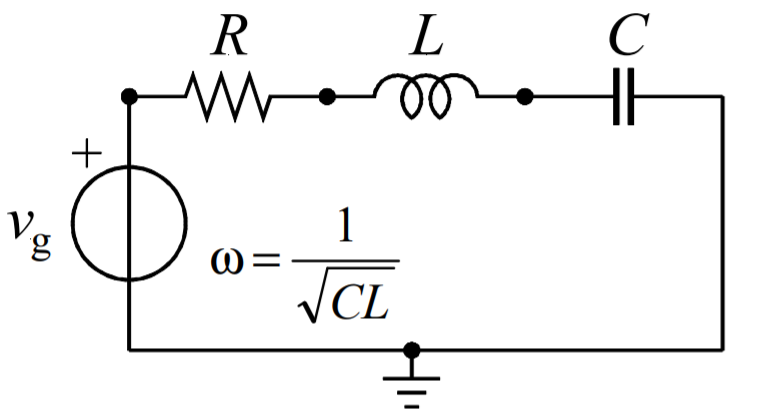
\includegraphics[scale = 0.45]{Figure1.PNG}\\
       Figure 1: RLC circuit.
   \end{center} 

    \textbf{Step 1.1.} Mark all nodes in the circuit with integer values
starting from 0 (Figure 2). \\

    \begin{center}
   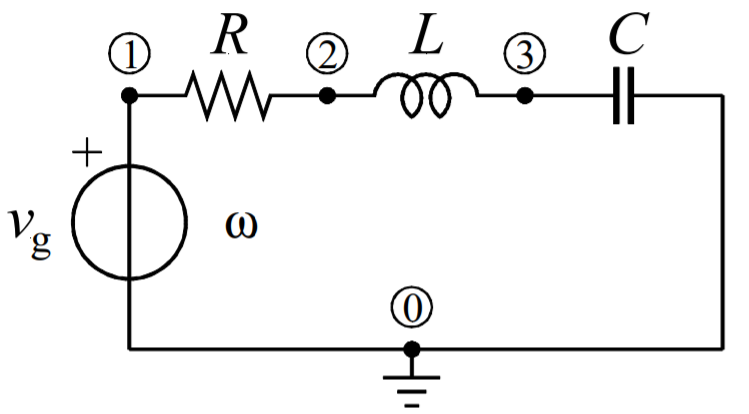
\includegraphics[scale = 0.45]{Figure2.PNG}\\
       Figure 2: RLC circuit with marked nodes.
   \end{center} 

    

    \textbf{Step 1.2.} In order to solve this circuit, import the
{\setlength{\fboxsep}{2pt}\colorbox{LightGray}{\texttt{Circuit}}} class from symPyCAP and import SymPy.

    \begin{tcolorbox}[breakable, size=fbox, boxrule=1pt, pad at break*=1mm,colback=cellbackground, colframe=cellborder]
\prompt{In}{incolor}{1}{\boxspacing}
\begin{Verbatim}[commandchars=\\\{\}]
\PY{k+kn}{from} \PY{n+nn}{symPyCAP} \PY{k+kn}{import} \PY{n}{Circuit}
\PY{k+kn}{import} \PY{n+nn}{sympy}
\end{Verbatim}
\end{tcolorbox}

    \textbf{Step 1.3.} Create a list of the elements that make up the circuit.
Each element is listed in a specific format given in the documentation.

    \begin{tcolorbox}[breakable, size=fbox, boxrule=1pt, pad at break*=1mm,colback=cellbackground, colframe=cellborder]
\prompt{In}{incolor}{2}{\boxspacing}
\begin{Verbatim}[commandchars=\\\{\}]
\PY{n}{RLC\PYZus{}schematic} \PY{o}{=} \PY{p}{[}
    \PY{p}{[}\PY{l+s+s2}{\PYZdq{}}\PY{l+s+s2}{V}\PY{l+s+s2}{\PYZdq{}}\PY{p}{,}\PY{l+s+s2}{\PYZdq{}}\PY{l+s+s2}{Vg}\PY{l+s+s2}{\PYZdq{}}\PY{p}{,}\PY{l+m+mi}{1}\PY{p}{,}\PY{l+m+mi}{0}\PY{p}{]}\PY{p}{,}
    \PY{p}{[}\PY{l+s+s2}{\PYZdq{}}\PY{l+s+s2}{R}\PY{l+s+s2}{\PYZdq{}}\PY{p}{,}\PY{l+s+s2}{\PYZdq{}}\PY{l+s+s2}{R1}\PY{l+s+s2}{\PYZdq{}}\PY{p}{,}\PY{l+m+mi}{1}\PY{p}{,}\PY{l+m+mi}{2}\PY{p}{]}\PY{p}{,}
    \PY{p}{[}\PY{l+s+s2}{\PYZdq{}}\PY{l+s+s2}{C}\PY{l+s+s2}{\PYZdq{}}\PY{p}{,}\PY{l+s+s2}{\PYZdq{}}\PY{l+s+s2}{C1}\PY{l+s+s2}{\PYZdq{}}\PY{p}{,}\PY{l+m+mi}{2}\PY{p}{,}\PY{l+m+mi}{3}\PY{p}{,}\PY{l+s+s2}{\PYZdq{}}\PY{l+s+s2}{UC0}\PY{l+s+s2}{\PYZdq{}}\PY{p}{]}\PY{p}{,}
    \PY{p}{[}\PY{l+s+s2}{\PYZdq{}}\PY{l+s+s2}{L}\PY{l+s+s2}{\PYZdq{}}\PY{p}{,}\PY{l+s+s2}{\PYZdq{}}\PY{l+s+s2}{L1}\PY{l+s+s2}{\PYZdq{}}\PY{p}{,}\PY{l+m+mi}{3}\PY{p}{,}\PY{l+m+mi}{0}\PY{p}{,}\PY{l+s+s2}{\PYZdq{}}\PY{l+s+s2}{IL0}\PY{l+s+s2}{\PYZdq{}}\PY{p}{]}
\PY{p}{]}
\end{Verbatim}
\end{tcolorbox}

    \textbf{Step 1.4.} In addition to the list of elements, create all the
symbols needed to solve the circuit, as well as replacement symbols.

    \begin{tcolorbox}[breakable, size=fbox, boxrule=1pt, pad at break*=1mm,colback=cellbackground, colframe=cellborder]
\prompt{In}{incolor}{3}{\boxspacing}
\begin{Verbatim}[commandchars=\\\{\}]
\PY{n}{R}\PY{p}{,}\PY{n}{C}\PY{p}{,}\PY{n}{L}\PY{p}{,}\PY{n}{W} \PY{o}{=} \PY{n}{sympy}\PY{o}{.}\PY{n}{symbols}\PY{p}{(}\PY{l+s+s1}{\PYZsq{}}\PY{l+s+s1}{R,C,L,W}\PY{l+s+s1}{\PYZsq{}}\PY{p}{)}
\end{Verbatim}
\end{tcolorbox}

    \textbf{Step 1.5.} Create an instance of the Circuit class with the list
of elements {\setlength{\fboxsep}{2pt}\colorbox{LightGray}{\texttt{RLC\_schematic}}} as an argument.

    \begin{tcolorbox}[breakable, size=fbox, boxrule=1pt, pad at break*=1mm,colback=cellbackground, colframe=cellborder]
\prompt{In}{incolor}{4}{\boxspacing}
\begin{Verbatim}[commandchars=\\\{\}]
\PY{n}{RLC_circuit} \PY{o}{=} \PY{n}{Circuit}\PY{p}{(}\PY{n}{RLC\PYZus{}schematic}\PY{p}{)}
\end{Verbatim}
\end{tcolorbox}

    \textbf{Step 1.6.} Call {\setlength{\fboxsep}{2pt}\colorbox{LightGray}{\texttt{symPyCAP}}} method to solve the circuit, that is, to find the response. Pass the symbolic
values of the elements and the frequency.\\ \textbf{Note:}
{\setlength{\fboxsep}{2pt}\colorbox{LightGray}{\texttt{sympy.sqrt()}}} should be used, not {\setlength{\fboxsep}{2pt}\colorbox{LightGray}{\texttt{math.sqrt()}}}.

    \begin{tcolorbox}[breakable, size=fbox, boxrule=1pt, pad at break*=1mm,colback=cellbackground, colframe=cellborder]
\prompt{In}{incolor}{5}{\boxspacing}
\begin{Verbatim}[commandchars=\\\{\}]
\PY{n}{RLC_circuit}\PY{o}{.}\PY{n}{symPyCAP}\PY{p}{(}\PY{n}{w} \PY{o}{=} \PY{l+m+mi}{1}\PY{o}{/}\PY{p}{(}\PY{n}{sympy}\PY{o}{.}\PY{n}{sqrt}\PY{p}{(}\PY{n}{L}\PY{o}{*}\PY{n}{C}\PY{p}{)}\PY{p}{)}\PY{p}{,} \PY{n}{replacement} \PY{o}{=} \PY{p}{\PYZob{}}\PY{l+s+s2}{\PYZdq{}}\PY{l+s+s2}{R1}\PY{l+s+s2}{\PYZdq{}} \PY{p}{:} \PY{n}{R}\PY{p}{,} \PY{l+s+s2}{\PYZdq{}}\PY{l+s+s2}{C1}\PY{l+s+s2}{\PYZdq{}} \PY{p}{:} \PY{n}{C}\PY{p}{,} \PY{l+s+s2}{\PYZdq{}}\PY{l+s+s2}{L1}\PY{l+s+s2}{\PYZdq{}} \PY{p}{:} \PY{n}{L}\PY{p}{\PYZcb{}}\PY{p}{)}
\end{Verbatim}
\end{tcolorbox}

    \textbf{Step 1.7.} After the method has solved the circuit, print the
solution.\\ \textbf{Note:} printing the solution that does not include the
replacement can be done by the {\setlength{\fboxsep}{2pt}\colorbox{LightGray}{\texttt{print\_solutions()}}} method.

    \begin{tcolorbox}[breakable, size=fbox, boxrule=1pt, pad at break*=1mm,colback=cellbackground, colframe=cellborder]
\prompt{In}{incolor}{6}{\boxspacing}
\begin{Verbatim}[commandchars=\\\{\}]
\PY{n}{RLC_circuit}\PY{o}{.}\PY{n}{print\PYZus{}specific\PYZus{}solutions}\PY{p}{(}\PY{p}{)}
\end{Verbatim}
\end{tcolorbox}

    \begin{Verbatim}[commandchars=\\\{\}]
V1 : Vg

V2 : 0

V3 : I*Vg*(C*L)**(3/2)/(C**2*L*R)

IVg : -Vg/R

    \end{Verbatim}
    
    \textbf{Note:} The solution doesn't contain intial conditions of capacitor and coil because of $jw$ analysis.\\ \textbf{Note:} $Vg$ is the rms value of the sinusoidal voltage source with the angular frequency $w = \displaystyle \frac{1}{\sqrt{LC}}$
    

    \textbf{Step 1.8.} It is possible to print the circuit specifications.

    \begin{tcolorbox}[breakable, size=fbox, boxrule=1pt, pad at break*=1mm,colback=cellbackground, colframe=cellborder]
\prompt{In}{incolor}{7}{\boxspacing}
\begin{Verbatim}[commandchars=\\\{\}]
\PY{n}{RLC_circuit}\PY{o}{.}\PY{n}{electric\PYZus{}circuit\PYZus{}specifications}\PY{p}{(}\PY{p}{)}
\end{Verbatim}
\end{tcolorbox}

    \begin{Verbatim}[commandchars=\\\{\}]
Circuit specifications:
Number of nodes: 4
Input elements:
['V', 'Vg', 1, 0]
['R', 'R1', 1, 2]
['C', 'C1', 2, 3, 'UC0']
['L', 'L1', 3, 0, 'IL0']
Replacement rule:  \{'R1': R, 'C1': C, 'L1': L\}
Equations:  [IVg + (V1 - V2)/R1, I*C1*(V2 - V3)/sqrt(C*L) + (-V1 + V2)/R1,
I*C1*(-V2 + V3)/sqrt(C*L) - I*V3*sqrt(C*L)/L1, -Vg + V1]
Variables:  [V1, V2, V3, IVg]
Frequency:  1/sqrt(C*L)

    \end{Verbatim}

    \begin{center}\rule{0.5\linewidth}{0.5pt}\end{center}

    \hypertarget{example-2-simple-capacitor-circuit}{%
\section*{\texorpdfstring{Example 2: Simple capacitor circuit
}{Example 2: Simple capacitor circuit }}\label{example2}}

A simple capacitor circuit is shown in Figure 3. The generator voltage is a step function of strength \textbf{\textit{Vstep}}. The capacitor is initially charged and its preinitial voltage, that is the initial condition, is \textbf{\textit{V0}}. Current of the ideal voltage source is presented to specify the reference direction.

    \begin{center}
   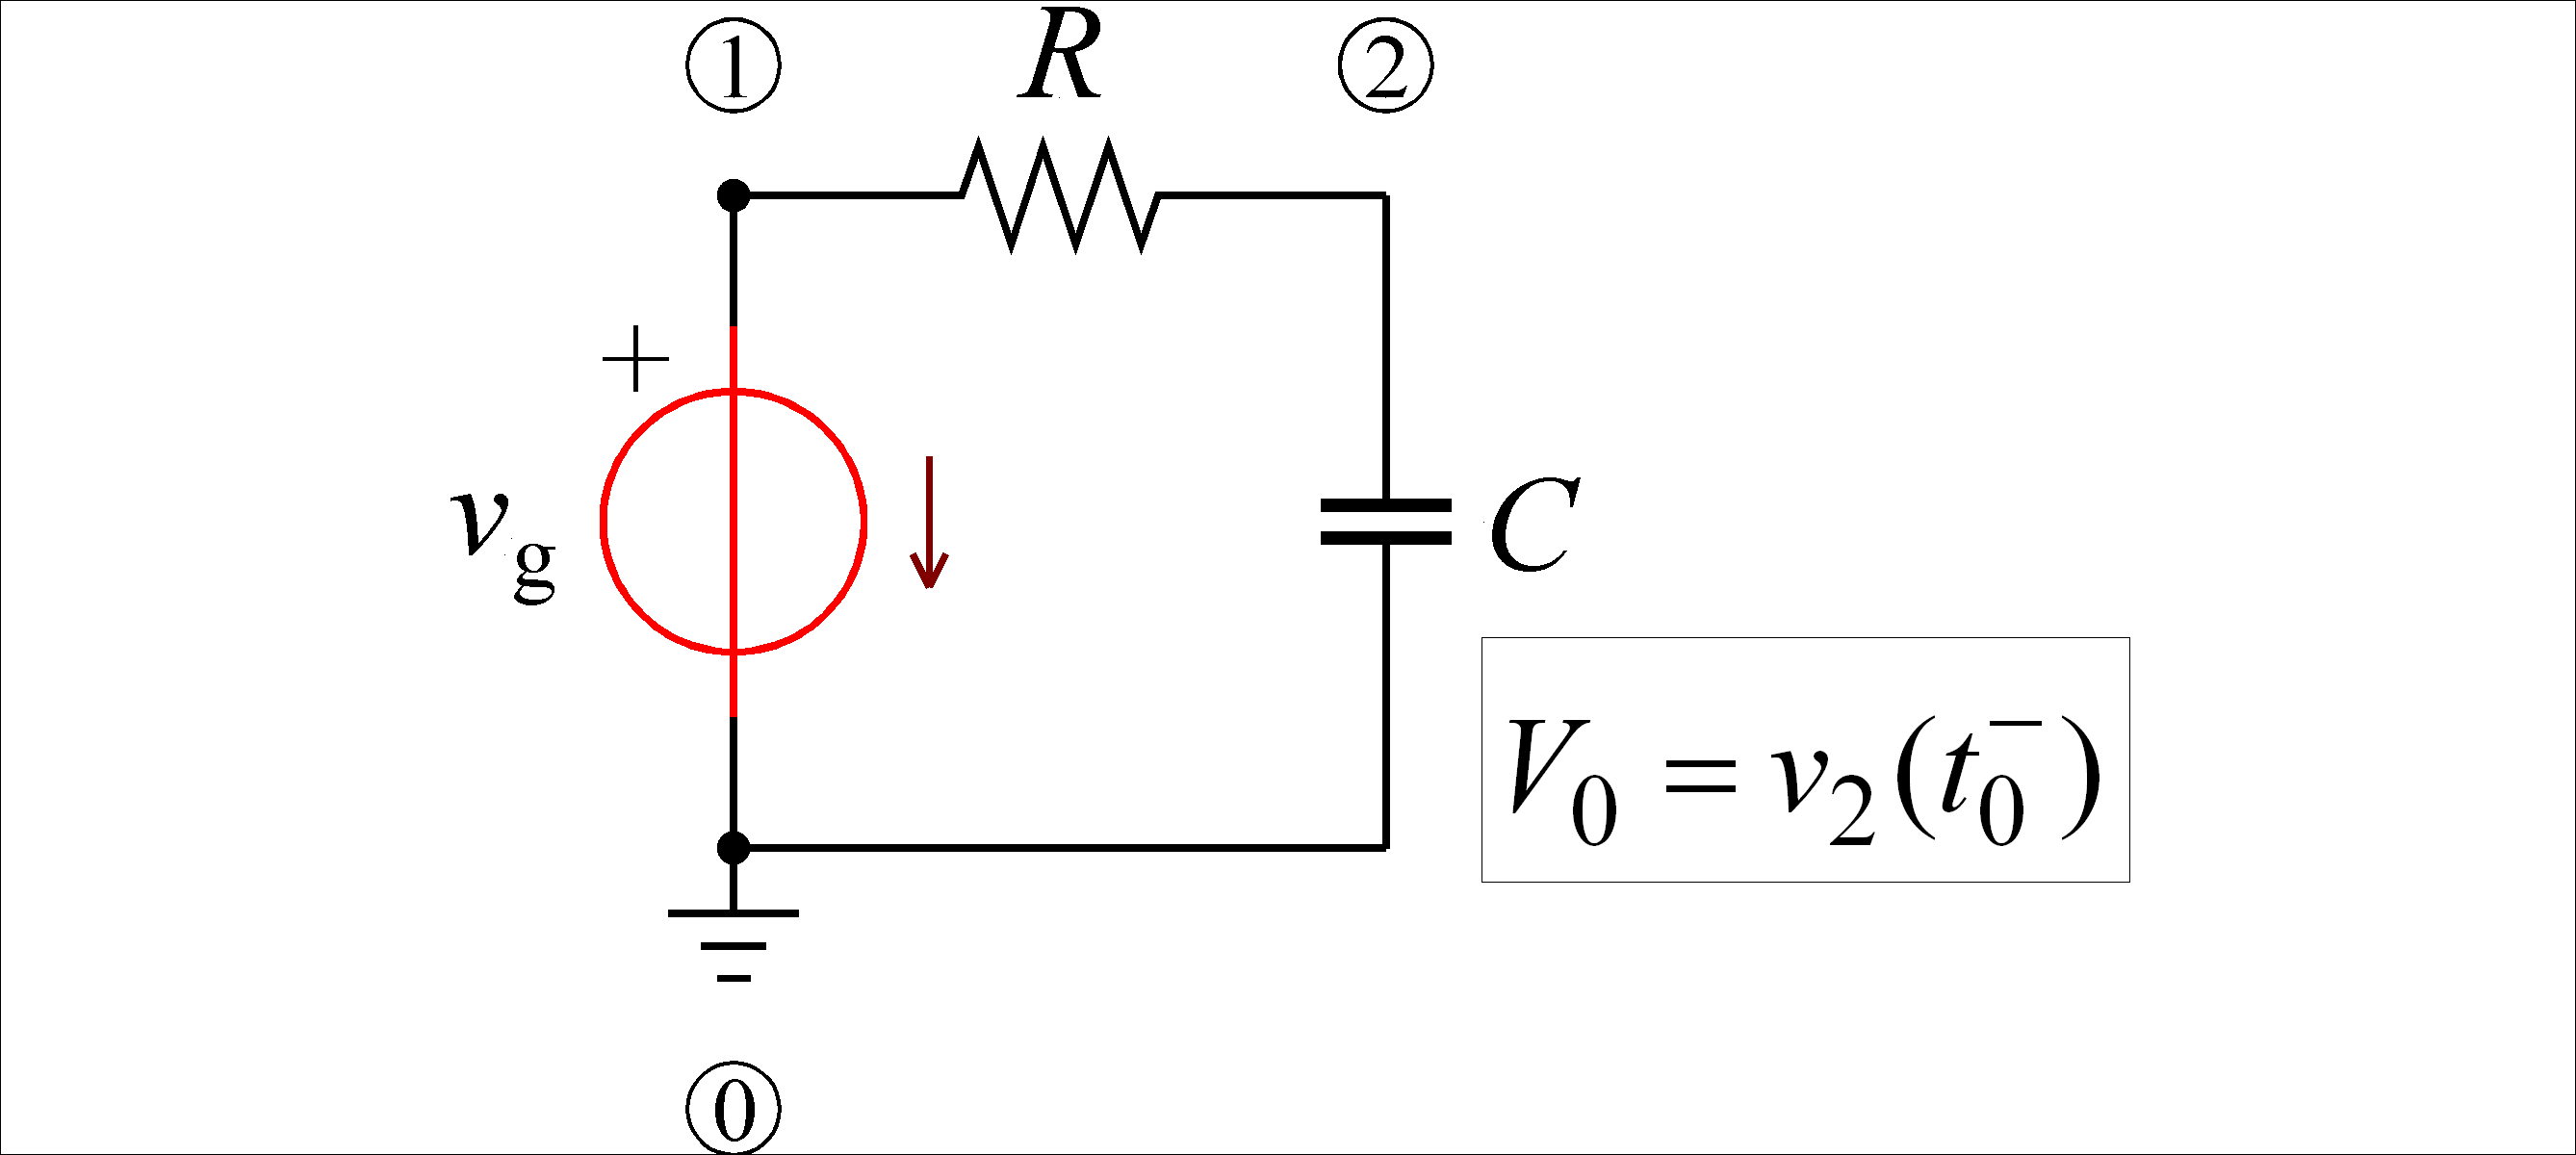
\includegraphics[scale = 0.6]{Figure3.png}\\
       Figure 3: Simple capacitor circuit.
   \end{center} 
    

    \textbf{Step 2.1.} Repeat steps 1.2 - 1.7.

    \begin{tcolorbox}[breakable, size=fbox, boxrule=1pt, pad at break*=1mm,colback=cellbackground, colframe=cellborder]
\prompt{In}{incolor}{8}{\boxspacing}
\begin{Verbatim}[commandchars=\\\{\}]
\PY{k+kn}{from} \PY{n+nn}{symPyCAP} \PY{k+kn}{import} \PY{n}{Circuit}
\PY{k+kn}{from} \PY{n+nn}{sympy} \PY{k+kn}{import} \PY{o}{*}
\end{Verbatim}
\end{tcolorbox}

    \textbf{Note:} Symbols like \textbf{\textit{I[id]}}, w, omega, r, replacement, \textbf{\textit{V0}},
\textbf{\textit{V1}}, \ldots{} are reserved symbols and must not be used for either symbol ids or for values in
replacement rule list.

    \begin{tcolorbox}[breakable, size=fbox, boxrule=1pt, pad at break*=1mm,colback=cellbackground, colframe=cellborder]
\prompt{In}{incolor}{9}{\boxspacing}
\begin{Verbatim}[commandchars=\\\{\}]
\PY{n}{Simple\PYZus{}capacitor\PYZus{}schematic} \PY{o}{=} \PY{p}{[}
    \PY{p}{[}\PY{l+s+s2}{\PYZdq{}}\PY{l+s+s2}{V}\PY{l+s+s2}{\PYZdq{}}\PY{p}{,}\PY{l+s+s2}{\PYZdq{}}\PY{l+s+s2}{Vg}\PY{l+s+s2}{\PYZdq{}}\PY{p}{,}\PY{l+m+mi}{1}\PY{p}{,}\PY{l+m+mi}{0}\PY{p}{]}\PY{p}{,}
    \PY{p}{[}\PY{l+s+s2}{\PYZdq{}}\PY{l+s+s2}{R}\PY{l+s+s2}{\PYZdq{}}\PY{p}{,}\PY{l+s+s2}{\PYZdq{}}\PY{l+s+s2}{R1}\PY{l+s+s2}{\PYZdq{}}\PY{p}{,}\PY{l+m+mi}{1}\PY{p}{,}\PY{l+m+mi}{2}\PY{p}{]}\PY{p}{,}
    \PY{p}{[}\PY{l+s+s2}{\PYZdq{}}\PY{l+s+s2}{C}\PY{l+s+s2}{\PYZdq{}}\PY{p}{,}\PY{l+s+s2}{\PYZdq{}}\PY{l+s+s2}{C1}\PY{l+s+s2}{\PYZdq{}}\PY{p}{,}\PY{l+m+mi}{2}\PY{p}{,}\PY{l+m+mi}{0}\PY{p}{,}\PY{l+s+s2}{\PYZdq{}}\PY{l+s+s2}{VC0}\PY{l+s+s2}{\PYZdq{}}\PY{p}{]}
\PY{p}{]}
\end{Verbatim}
\end{tcolorbox}



    \begin{tcolorbox}[breakable, size=fbox, boxrule=1pt, pad at break*=1mm,colback=cellbackground, colframe=cellborder]
\prompt{In}{incolor}{10}{\boxspacing}
\begin{Verbatim}[commandchars=\\\{\}]
\PY{n}{Vstep}\PY{p}{,}\PY{n}{s}\PY{p}{,}\PY{n}{t} \PY{o}{=} \PY{n}{sympy}\PY{o}{.}\PY{n}{symbols}\PY{p}{(}\PY{l+s+s1}{\PYZsq{}}\PY{l+s+s1}{Vstep,s,t}\PY{l+s+s1}{\PYZsq{}}\PY{p}{)}
\PY{n}{R} \PY{o}{=} \PY{n}{sympy}\PY{o}{.}\PY{n}{Symbol}\PY{p}{(}\PY{l+s+s1}{\PYZsq{}}\PY{l+s+s1}{R}\PY{l+s+s1}{\PYZsq{}}\PY{p}{,} \PY{n}{positive}\PY{o}{=}\PY{k+kc}{True}\PY{p}{)}
\PY{n}{C} \PY{o}{=} \PY{n}{sympy}\PY{o}{.}\PY{n}{Symbol}\PY{p}{(}\PY{l+s+s1}{\PYZsq{}}\PY{l+s+s1}{C}\PY{l+s+s1}{\PYZsq{}}\PY{p}{,} \PY{n}{positive}\PY{o}{=}\PY{k+kc}{True}\PY{p}{)}
\end{Verbatim}
\end{tcolorbox}

    \begin{tcolorbox}[breakable, size=fbox, boxrule=1pt, pad at break*=1mm,colback=cellbackground, colframe=cellborder]
\prompt{In}{incolor}{11}{\boxspacing}
\begin{Verbatim}[commandchars=\\\{\}]
\PY{n}{simple_capacitor_circuit} \PY{o}{=} \PY{n}{Circuit}\PY{p}{(}\PY{n}{Simple\PYZus{}capacitor\PYZus{}schematic}\PY{p}{)}
\end{Verbatim}
\end{tcolorbox}

    \textbf{Note:} calling {\setlength{\fboxsep}{2pt}\colorbox{LightGray}{\texttt{symPyCAP}}} without the frequency specification (\(w\)), solves the circuit in the \textbf{\textit{s}}-domain, the Unilateral (one-sided) Laplace Transform domain.

    \begin{tcolorbox}[breakable, size=fbox, boxrule=1pt, pad at break*=1mm,colback=cellbackground, colframe=cellborder]
\prompt{In}{incolor}{12}{\boxspacing}
\begin{Verbatim}[commandchars=\\\{\}]
\PY{n}{simple_capacitor_circuit}\PY{o}{.}\PY{n}{symPyCAP}\PY{p}{(}\PY{n}{replacement} \PY{o}{=} \PY{p}{\PYZob{}}\PY{l+s+s2}{\PYZdq{}}\PY{l+s+s2}{R1}\PY{l+s+s2}{\PYZdq{}} \PY{p}{:} \PY{n}{R}\PY{p}{,} \PY{l+s+s2}{\PYZdq{}}\PY{l+s+s2}{C1}\PY{l+s+s2}{\PYZdq{}} \PY{p}{:} \PY{n}{C}\PY{p}{,} \PY{l+s+s2}{\PYZdq{}}\PY{l+s+s2}{Vg}\PY{l+s+s2}{\PYZdq{}} \PY{p}{:} \PY{n}{Vstep}\PY{o}{/}\PY{n}{s}\PY{p}{\PYZcb{}}\PY{p}{)}
\end{Verbatim}
\end{tcolorbox}

    \textbf{Note:} The Laplace Transform of the source voltage is Vstep/s, where s represents the complex frequency, that is the Laplace Variable.

    \begin{tcolorbox}[breakable, size=fbox, boxrule=1pt, pad at break*=1mm,colback=cellbackground, colframe=cellborder]
\prompt{In}{incolor}{13}{\boxspacing}
\begin{Verbatim}[commandchars=\\\{\}]
\PY{n}{simple_capacitor_circuit}\PY{o}{.}\PY{n}{print\PYZus{}specific\PYZus{}solutions}\PY{p}{(}\PY{p}{)}
\end{Verbatim}
\end{tcolorbox}

    \begin{Verbatim}[commandchars=\\\{\}]
V1 : Vstep/s

V2 : (C*R*VC0*s + Vstep)/(s*(C*R*s + 1))

IVg : C*(VC0 - Vstep)/(C*R*s + 1)

    \end{Verbatim}

    \textbf{Step 2.2.} The time-domain capacitor voltage, for t
\textgreater{} 0, can be computed by SymPy's Inverse Laplace Transform
function.\\ \textbf{Note:} The getter {\setlength{\fboxsep}{2pt}\colorbox{LightGray}{\texttt{get\_specific\_solutions()}}} 
returns the dictionary of specific solutions which can be directly
indexed.

    \begin{tcolorbox}[breakable, size=fbox, boxrule=1pt, pad at break*=1mm,colback=cellbackground, colframe=cellborder]
\prompt{In}{incolor}{14}{\boxspacing}
\begin{Verbatim}[commandchars=\\\{\}]
\PY{n}{Uct} \PY{o}{=} \PY{n}{inverse\PYZus{}laplace\PYZus{}transform}\PY{p}{(}\PY{n}{system}\PY{o}{.}\PY{n}{get\PYZus{}specific\PYZus{}solutions}\PY{p}{(}\PY{p}{)}\PY{p}{[}\PY{l+s+s2}{\PYZdq{}}\PY{l+s+s2}{V2}\PY{l+s+s2}{\PYZdq{}}\PY{p}{]}\PY{p}{,}\PY{n}{s}\PY{p}{,}\PY{n}{t}\PY{p}{)}
\end{Verbatim}
\end{tcolorbox}

    \begin{tcolorbox}[breakable, size=fbox, boxrule=1pt, pad at break*=1mm,colback=cellbackground, colframe=cellborder]
\prompt{In}{incolor}{15}{\boxspacing}
\begin{Verbatim}[commandchars=\\\{\}]
\PY{n}{Uct}
\end{Verbatim}
\end{tcolorbox}
 
            
\prompt{Out}{outcolor}{15}{}
    
    $\displaystyle \left(VC_{0} + Vstep e^{\frac{t}{C R}} - Vstep\right) e^{- \frac{t}{C R}} \theta\left(t\right)$

    

    \begin{center}\rule{0.5\linewidth}{0.5pt}\end{center}

    \hypertarget{example-3-ota-c-operational-transconductance-amplifier-with-capacitors}{%
\section*{\texorpdfstring{Example 3: OTA-C (Operational
Transconductance Amplifier with Capacitors)
}{Example 3: OTA-C (Operational Transconductance Amplifier with Capacitors) }}\label{example3}}

An \textbf{OTA-C} (\textbf{O}PERATIONAL \textbf{T}RANSCONDUCTANCE
\textbf{A}MPLIFIER with \textbf{C}APACITORS) lowpass and bandpass
\(2^{nd}\)- order filter realization (Figure 4.) is to be solved.

    \begin{center}
   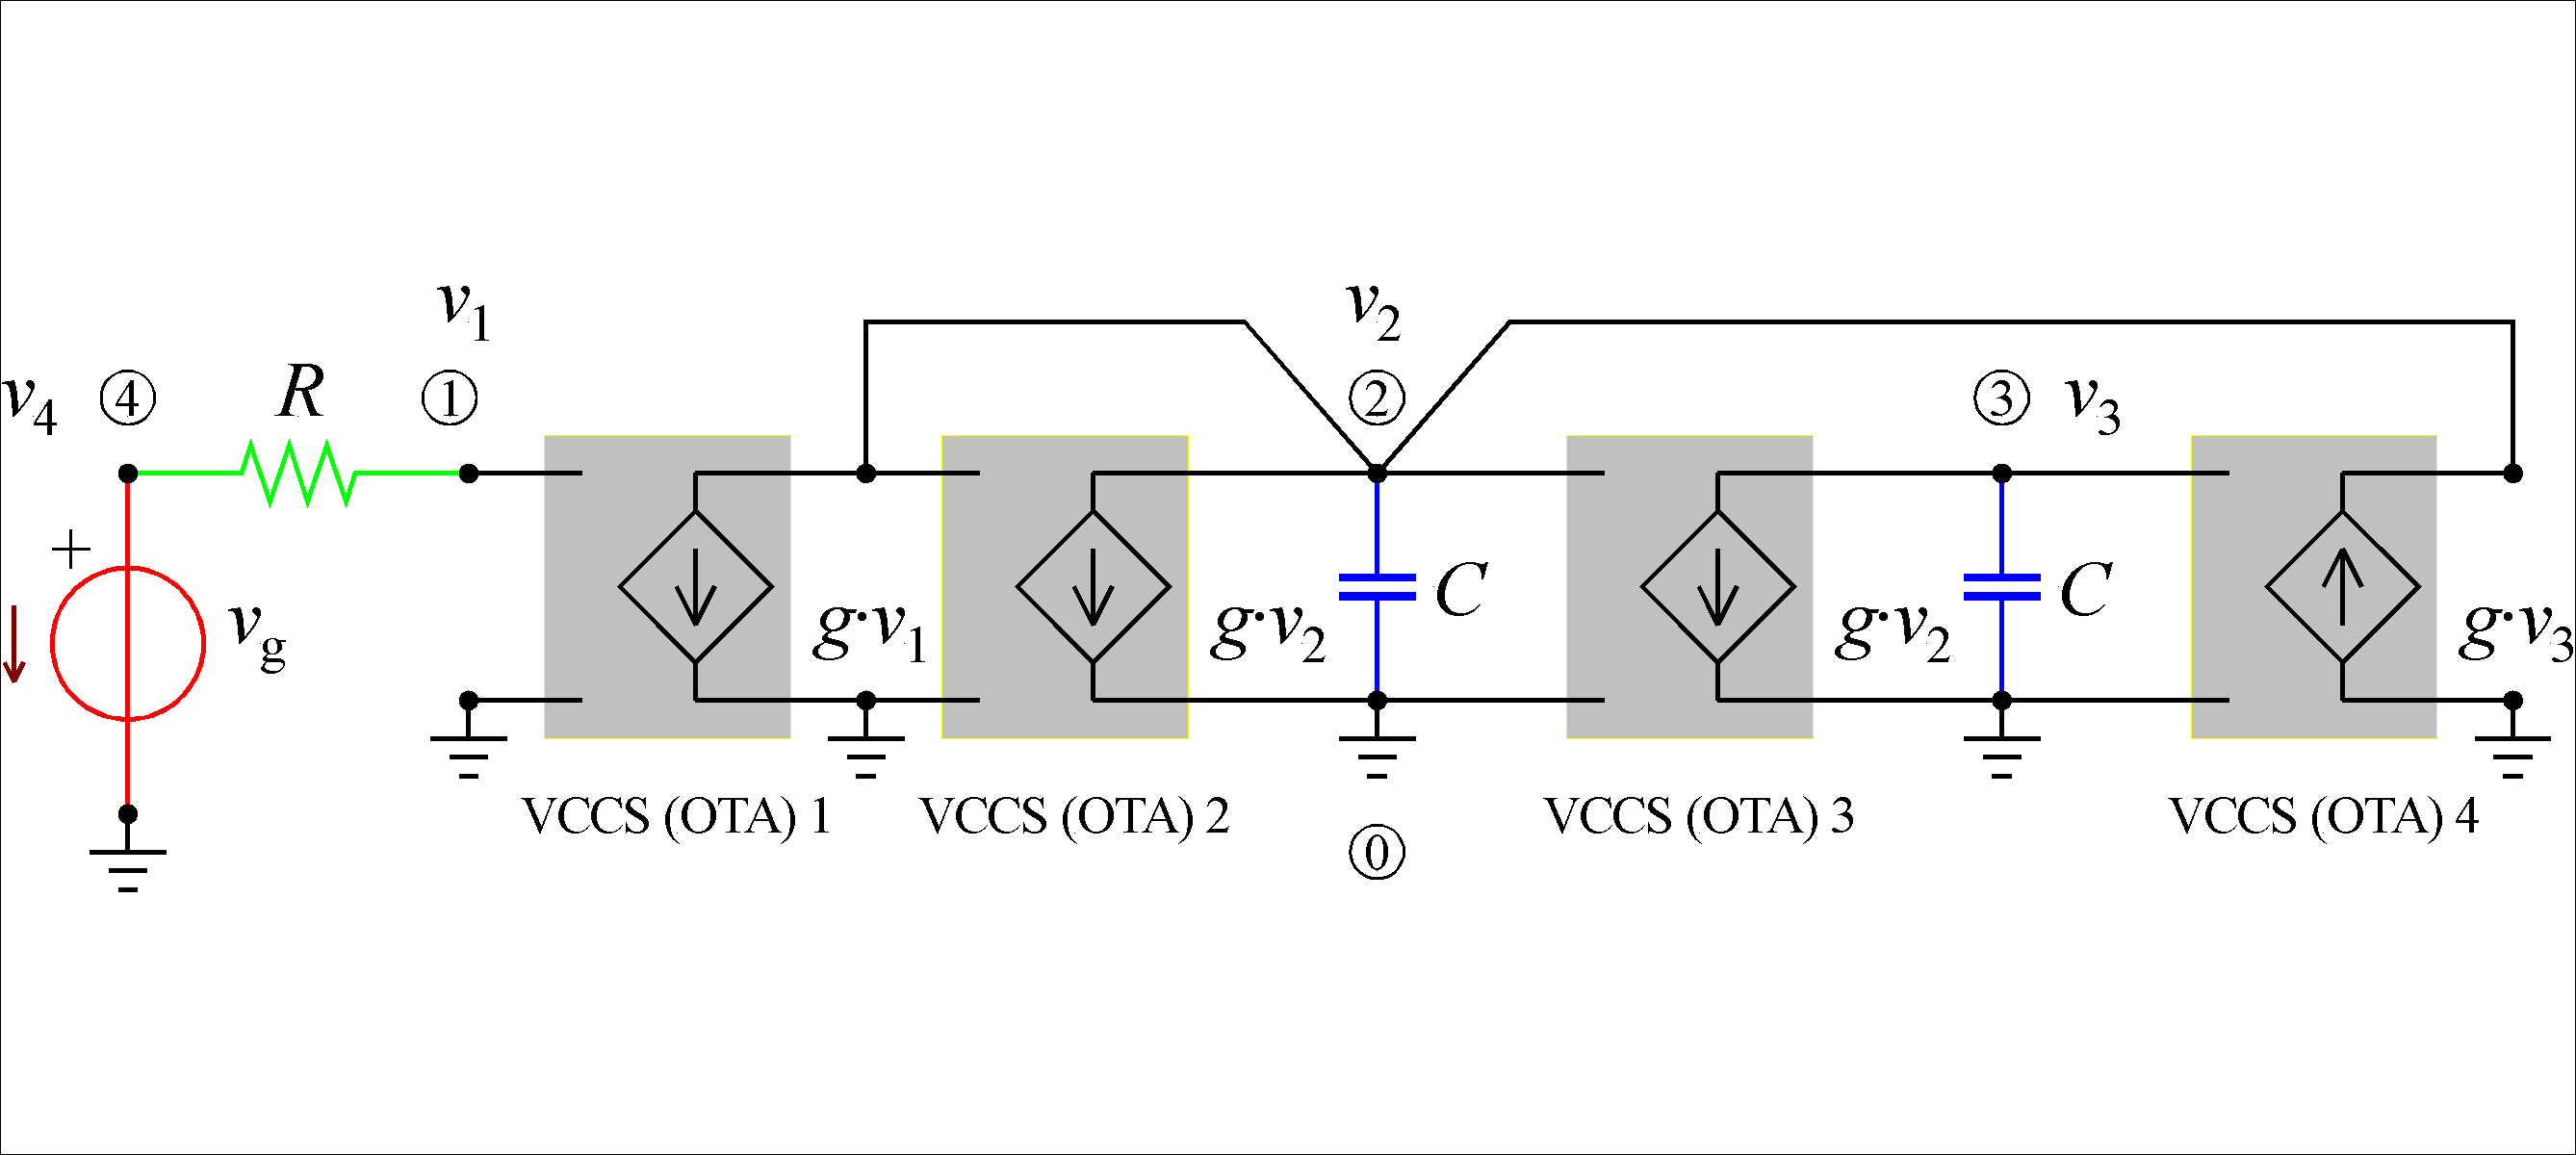
\includegraphics[scale = 0.9]{Figure4.png}\\
       Figure 4: OTA-C (Operational Transconductance Amplifier with
Capacitors).
   \end{center} 

    \textbf{Step 3.1.} Repeat steps 1.2-1.7.

    \begin{tcolorbox}[breakable, size=fbox, boxrule=1pt, pad at break*=1mm,colback=cellbackground, colframe=cellborder]
\prompt{In}{incolor}{16}{\boxspacing}
\begin{Verbatim}[commandchars=\\\{\}]
\PY{k+kn}{from} \PY{n+nn}{symPyCAP} \PY{k+kn}{import} \PY{n}{Circuit}
\PY{k+kn}{from} \PY{n+nn}{sympy} \PY{k+kn}{import} \PY{o}{*}
\end{Verbatim}
\end{tcolorbox}

    \begin{tcolorbox}[breakable, size=fbox, boxrule=1pt, pad at break*=1mm,colback=cellbackground, colframe=cellborder]
\prompt{In}{incolor}{17}{\boxspacing}
\begin{Verbatim}[commandchars=\\\{\}]
\PY{n}{OTA\PYZus{}C\PYZus{}schematic} \PY{o}{=} \PY{p}{[}
    \PY{p}{[}\PY{l+s+s2}{\PYZdq{}}\PY{l+s+s2}{V}\PY{l+s+s2}{\PYZdq{}}\PY{p}{,} \PY{l+s+s2}{\PYZdq{}}\PY{l+s+s2}{Vg}\PY{l+s+s2}{\PYZdq{}}\PY{p}{,} \PY{l+m+mi}{4}\PY{p}{,} \PY{l+m+mi}{0}\PY{p}{]}\PY{p}{,}
    \PY{p}{[}\PY{l+s+s2}{\PYZdq{}}\PY{l+s+s2}{R}\PY{l+s+s2}{\PYZdq{}}\PY{p}{,} \PY{l+s+s2}{\PYZdq{}}\PY{l+s+s2}{R1}\PY{l+s+s2}{\PYZdq{}}\PY{p}{,} \PY{l+m+mi}{4}\PY{p}{,} \PY{l+m+mi}{1}\PY{p}{]}\PY{p}{,}
    \PY{p}{[}\PY{l+s+s2}{\PYZdq{}}\PY{l+s+s2}{VCCS}\PY{l+s+s2}{\PYZdq{}}\PY{p}{,} \PY{l+s+s2}{\PYZdq{}}\PY{l+s+s2}{OTA1}\PY{l+s+s2}{\PYZdq{}}\PY{p}{,} \PY{p}{[}\PY{l+m+mi}{1}\PY{p}{,}\PY{l+m+mi}{0}\PY{p}{]}\PY{p}{,} \PY{p}{[}\PY{l+m+mi}{2}\PY{p}{,}\PY{l+m+mi}{0}\PY{p}{]}\PY{p}{,} \PY{l+s+s2}{\PYZdq{}}\PY{l+s+s2}{g}\PY{l+s+s2}{\PYZdq{}}\PY{p}{]}\PY{p}{,}
    \PY{p}{[}\PY{l+s+s2}{\PYZdq{}}\PY{l+s+s2}{VCCS}\PY{l+s+s2}{\PYZdq{}}\PY{p}{,} \PY{l+s+s2}{\PYZdq{}}\PY{l+s+s2}{OTA2}\PY{l+s+s2}{\PYZdq{}}\PY{p}{,} \PY{p}{[}\PY{l+m+mi}{2}\PY{p}{,}\PY{l+m+mi}{0}\PY{p}{]}\PY{p}{,} \PY{p}{[}\PY{l+m+mi}{2}\PY{p}{,}\PY{l+m+mi}{0}\PY{p}{]}\PY{p}{,} \PY{l+s+s2}{\PYZdq{}}\PY{l+s+s2}{g}\PY{l+s+s2}{\PYZdq{}}\PY{p}{]}\PY{p}{,}
    \PY{p}{[}\PY{l+s+s2}{\PYZdq{}}\PY{l+s+s2}{VCCS}\PY{l+s+s2}{\PYZdq{}}\PY{p}{,} \PY{l+s+s2}{\PYZdq{}}\PY{l+s+s2}{OTA3}\PY{l+s+s2}{\PYZdq{}}\PY{p}{,} \PY{p}{[}\PY{l+m+mi}{2}\PY{p}{,}\PY{l+m+mi}{0}\PY{p}{]}\PY{p}{,} \PY{p}{[}\PY{l+m+mi}{3}\PY{p}{,}\PY{l+m+mi}{0}\PY{p}{]}\PY{p}{,} \PY{l+s+s2}{\PYZdq{}}\PY{l+s+s2}{g}\PY{l+s+s2}{\PYZdq{}}\PY{p}{]}\PY{p}{,}
    \PY{p}{[}\PY{l+s+s2}{\PYZdq{}}\PY{l+s+s2}{VCCS}\PY{l+s+s2}{\PYZdq{}}\PY{p}{,} \PY{l+s+s2}{\PYZdq{}}\PY{l+s+s2}{OTA4}\PY{l+s+s2}{\PYZdq{}}\PY{p}{,} \PY{p}{[}\PY{l+m+mi}{3}\PY{p}{,}\PY{l+m+mi}{0}\PY{p}{]}\PY{p}{,} \PY{p}{[}\PY{l+m+mi}{0}\PY{p}{,}\PY{l+m+mi}{2}\PY{p}{]}\PY{p}{,} \PY{l+s+s2}{\PYZdq{}}\PY{l+s+s2}{g}\PY{l+s+s2}{\PYZdq{}}\PY{p}{]}\PY{p}{,}
    \PY{p}{[}\PY{l+s+s2}{\PYZdq{}}\PY{l+s+s2}{C}\PY{l+s+s2}{\PYZdq{}}\PY{p}{,} \PY{l+s+s2}{\PYZdq{}}\PY{l+s+s2}{C1}\PY{l+s+s2}{\PYZdq{}}\PY{p}{,} \PY{l+m+mi}{2}\PY{p}{,} \PY{l+m+mi}{0}\PY{p}{]}\PY{p}{,}
    \PY{p}{[}\PY{l+s+s2}{\PYZdq{}}\PY{l+s+s2}{C}\PY{l+s+s2}{\PYZdq{}}\PY{p}{,} \PY{l+s+s2}{\PYZdq{}}\PY{l+s+s2}{C2}\PY{l+s+s2}{\PYZdq{}}\PY{p}{,} \PY{l+m+mi}{3}\PY{p}{,} \PY{l+m+mi}{0}\PY{p}{]}
\PY{p}{]}
\end{Verbatim}
\end{tcolorbox}

    \begin{tcolorbox}[breakable, size=fbox, boxrule=1pt, pad at break*=1mm,colback=cellbackground, colframe=cellborder]
\prompt{In}{incolor}{18}{\boxspacing}
\begin{Verbatim}[commandchars=\\\{\}]
\PY{n}{R}\PY{p}{,}\PY{n}{C} \PY{o}{=} \PY{n}{symbols}\PY{p}{(}\PY{l+s+s1}{\PYZsq{}}\PY{l+s+s1}{R,C}\PY{l+s+s1}{\PYZsq{}}\PY{p}{)}
\end{Verbatim}
\end{tcolorbox}

    \begin{tcolorbox}[breakable, size=fbox, boxrule=1pt, pad at break*=1mm,colback=cellbackground, colframe=cellborder]
\prompt{In}{incolor}{19}{\boxspacing}
\begin{Verbatim}[commandchars=\\\{\}]
\PY{n}{OTA_C_circuit} \PY{o}{=} \PY{n}{Circuit}\PY{p}{(}\PY{n}{OTA\PYZus{}C\PYZus{}schematic}\PY{p}{)}
\end{Verbatim}
\end{tcolorbox}

    \begin{tcolorbox}[breakable, size=fbox, boxrule=1pt, pad at break*=1mm,colback=cellbackground, colframe=cellborder]
\prompt{In}{incolor}{20}{\boxspacing}
\begin{Verbatim}[commandchars=\\\{\}]
\PY{n}{OTA_C_circuit}\PY{o}{.}\PY{n}{symPyCAP}\PY{p}{(}\PY{n}{replacement} \PY{o}{=} \PY{p}{\PYZob{}}\PY{l+s+s2}{\PYZdq{}}\PY{l+s+s2}{R1}\PY{l+s+s2}{\PYZdq{}} \PY{p}{:} \PY{n}{R}\PY{p}{,} \PY{l+s+s2}{\PYZdq{}}\PY{l+s+s2}{C1}\PY{l+s+s2}{\PYZdq{}} \PY{p}{:} \PY{n}{C}\PY{p}{,} \PY{l+s+s2}{\PYZdq{}}\PY{l+s+s2}{C2}\PY{l+s+s2}{\PYZdq{}} \PY{p}{:} \PY{n}{C}\PY{p}{\PYZcb{}}\PY{p}{)}
\end{Verbatim}
\end{tcolorbox}

    \begin{tcolorbox}[breakable, size=fbox, boxrule=1pt, pad at break*=1mm,colback=cellbackground, colframe=cellborder]
\prompt{In}{incolor}{21}{\boxspacing}
\begin{Verbatim}[commandchars=\\\{\}]
\PY{n}{OTA_C_circuit}\PY{o}{.}\PY{n}{print\PYZus{}specific\PYZus{}solutions}\PY{p}{(}\PY{p}{)}
\end{Verbatim}
\end{tcolorbox}

    \begin{Verbatim}[commandchars=\\\{\}]
V1 : Vg

V2 : -C*Vg*g*s/(C**2*s**2 + C*g*s + g**2)

V3 : Vg*g**2/(C**2*s**2 + C*g*s + g**2)

V4 : Vg

IVg : 0

    \end{Verbatim}

    \textbf{Step 3.2.} Use node voltages to calculate transfer functions.

    \begin{tcolorbox}[breakable, size=fbox, boxrule=1pt, pad at break*=1mm,colback=cellbackground, colframe=cellborder]
\prompt{In}{incolor}{22}{\boxspacing}
\begin{Verbatim}[commandchars=\\\{\}]
\PY{n}{Hs2bandpass} \PY{o}{=} \PY{n}{OTA_C_circuit}\PY{o}{.}\PY{n}{get\PYZus{}specific\PYZus{}solutions}\PY{p}{(}\PY{p}{)}\PY{p}{[}\PY{l+s+s1}{\PYZsq{}}\PY{l+s+s1}{V2}\PY{l+s+s1}{\PYZsq{}}\PY{p}{]}\PY{o}{/}\PY{n}{OTA_C_circuit}\PY{o}{.}\PY{n}{get\PYZus{}specific\PYZus{}solutions}\PY{p}{(}\PY{p}{)}\PY{p}{[}\PY{l+s+s1}{\PYZsq{}}\PY{l+s+s1}{V1}\PY{l+s+s1}{\PYZsq{}}\PY{p}{]} 
\end{Verbatim}
\end{tcolorbox}

    \begin{tcolorbox}[breakable, size=fbox, boxrule=1pt, pad at break*=1mm,colback=cellbackground, colframe=cellborder]
\prompt{In}{incolor}{23}{\boxspacing}
\begin{Verbatim}[commandchars=\\\{\}]
\PY{n}{Hs2bandpass}
\end{Verbatim}
\end{tcolorbox}
 
            
\prompt{Out}{outcolor}{23}{}
    
    $\displaystyle - \frac{C g s}{C^{2} s^{2} + C g s + g^{2}}$

    

    \begin{tcolorbox}[breakable, size=fbox, boxrule=1pt, pad at break*=1mm,colback=cellbackground, colframe=cellborder]
\prompt{In}{incolor}{24}{\boxspacing}
\begin{Verbatim}[commandchars=\\\{\}]
\PY{n}{Hs3lowpass} \PY{o}{=} \PY{n}{OTA_C_circuit}\PY{o}{.}\PY{n}{get\PYZus{}specific\PYZus{}solutions}\PY{p}{(}\PY{p}{)}\PY{p}{[}\PY{l+s+s1}{\PYZsq{}}\PY{l+s+s1}{V3}\PY{l+s+s1}{\PYZsq{}}\PY{p}{]}\PY{o}{/}\PY{n}{OTA_C_circuit}\PY{o}{.}\PY{n}{get\PYZus{}specific\PYZus{}solutions}\PY{p}{(}\PY{p}{)}\PY{p}{[}\PY{l+s+s1}{\PYZsq{}}\PY{l+s+s1}{V1}\PY{l+s+s1}{\PYZsq{}}\PY{p}{]}
\end{Verbatim}
\end{tcolorbox}

    \begin{tcolorbox}[breakable, size=fbox, boxrule=1pt, pad at break*=1mm,colback=cellbackground, colframe=cellborder]
\prompt{In}{incolor}{25}{\boxspacing}
\begin{Verbatim}[commandchars=\\\{\}]
\PY{n}{Hs3lowpass}
\end{Verbatim}
\end{tcolorbox}
 
            
\prompt{Out}{outcolor}{25}{}
    
    $\displaystyle \frac{g^{2}}{C^{2} s^{2} + C g s + g^{2}}$

    

    \begin{center}\rule{0.5\linewidth}{0.5pt}\end{center}

    \hypertarget{example-4-riordan-gyrator-network}{%
\section*{\texorpdfstring{Example 4: Riordan gyrator network
}{Example 4: Riordan gyrator network }}\label{example4}}

Synthetic inductor, which is realized with the Riordan gyrator network,
is shown in Figure 5. The proof-of-concept symbolic analysis follows.
The circuit is inductorless but, theoretically, the impedance seen by
the source is purely inductive.

    \begin{center}
   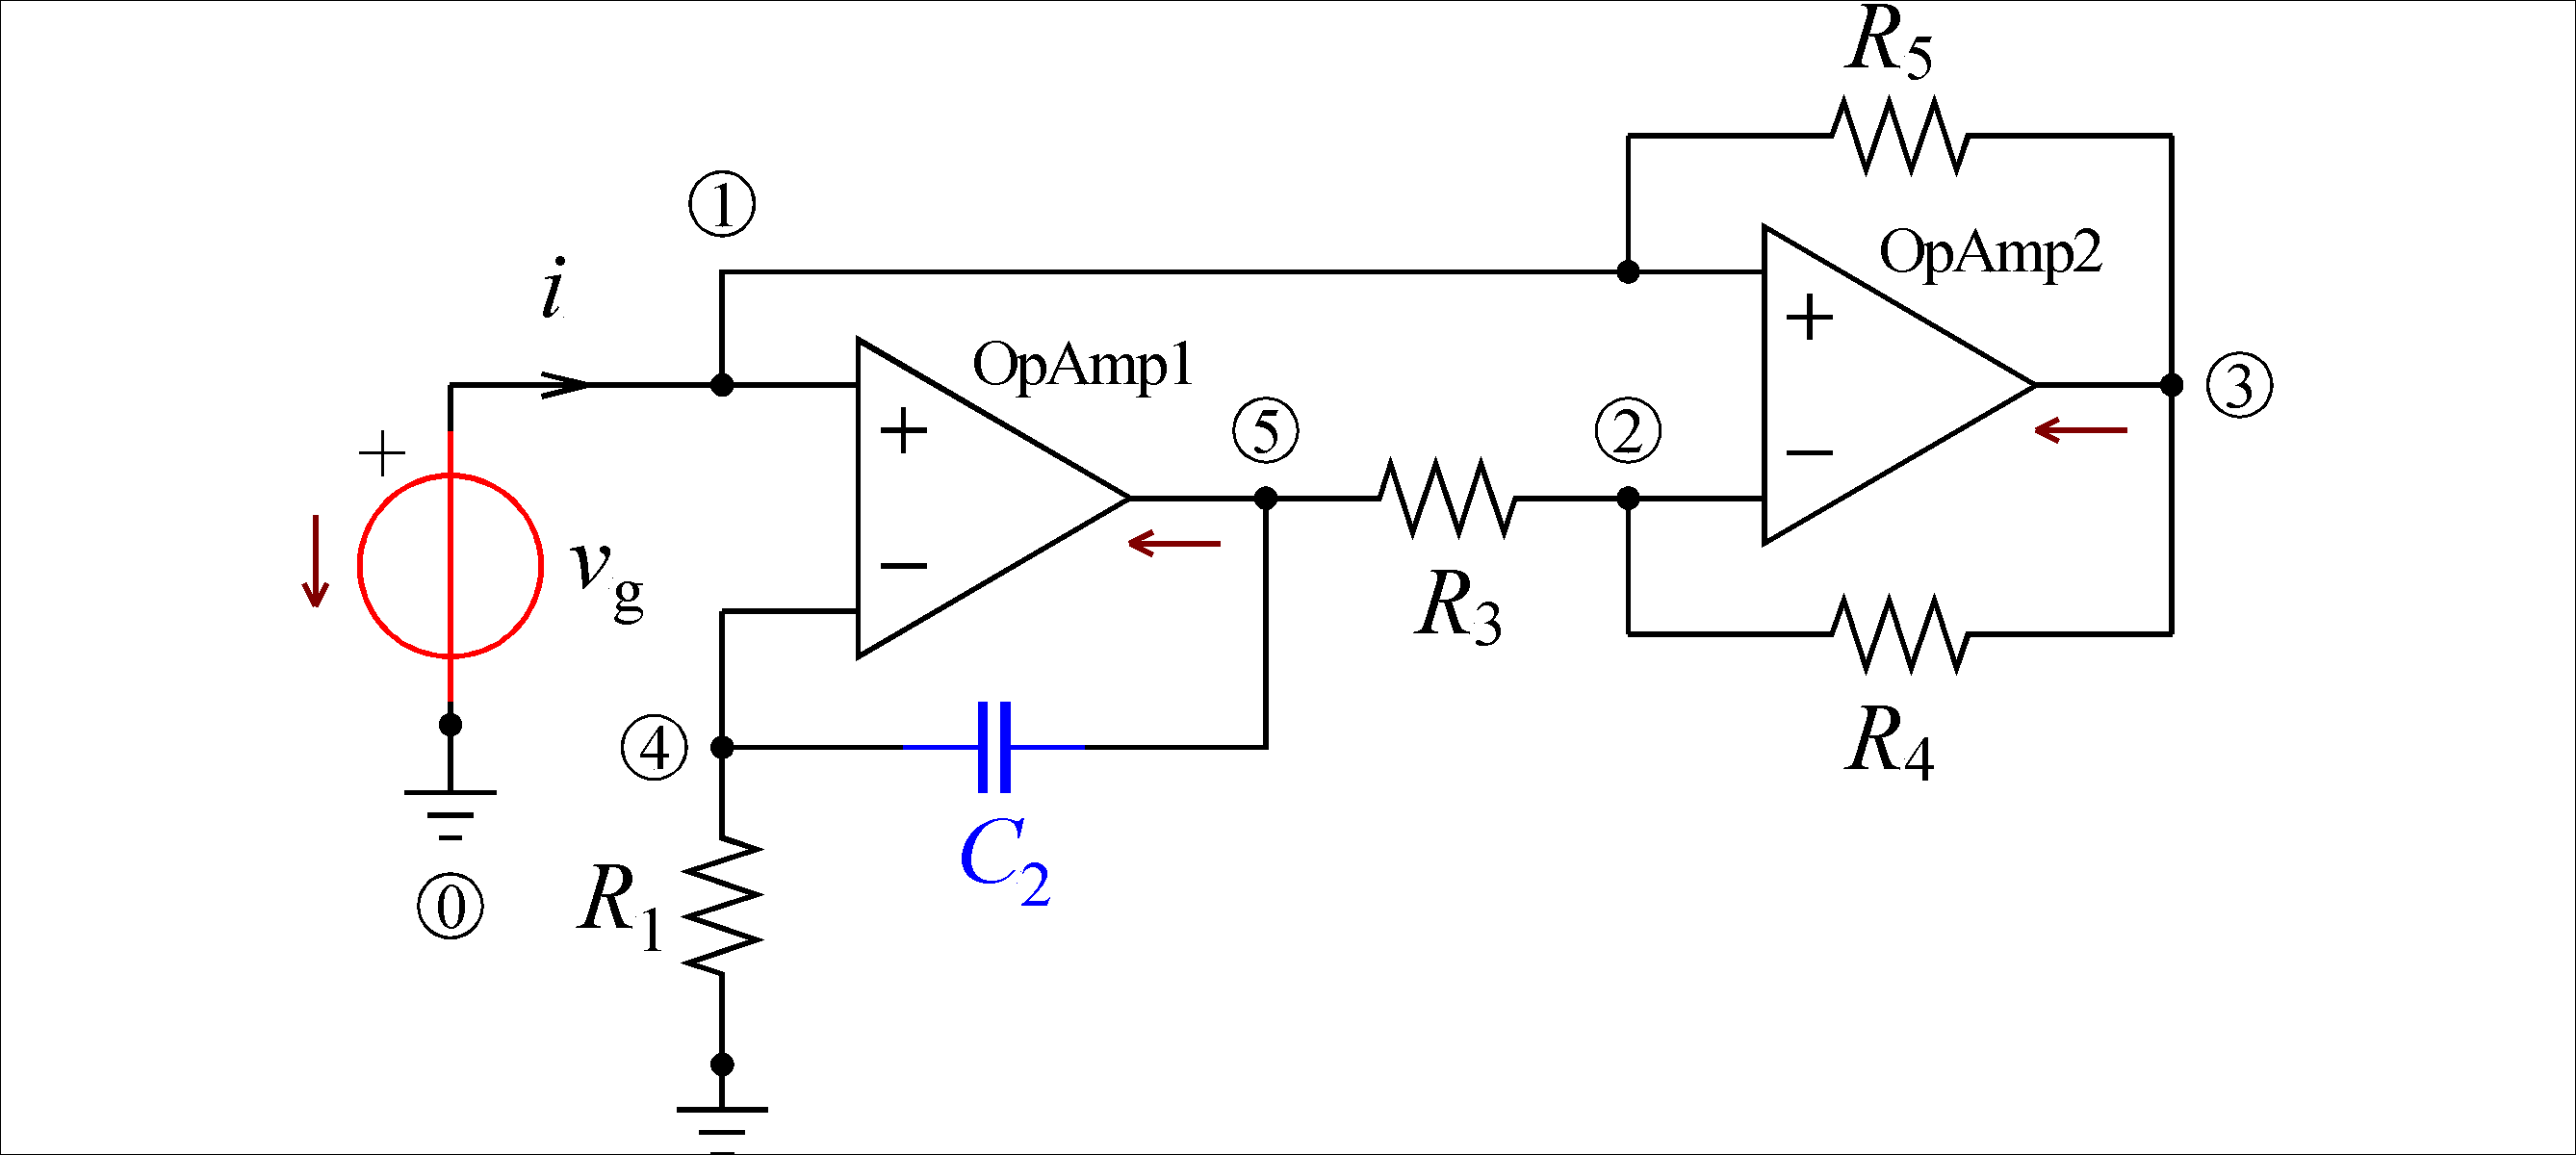
\includegraphics[scale = 0.75]{Figure5.png}\\
       Figure 5: Riordan gyrator network
   \end{center} 
    

    \textbf{Step 4.1.} Repeat steps 1.2.-1.7.

    \begin{tcolorbox}[breakable, size=fbox, boxrule=1pt, pad at break*=1mm,colback=cellbackground, colframe=cellborder]
\prompt{In}{incolor}{26}{\boxspacing}
\begin{Verbatim}[commandchars=\\\{\}]
\PY{k+kn}{from} \PY{n+nn}{symPyCAP} \PY{k+kn}{import} \PY{n}{Circuit}
\PY{k+kn}{from} \PY{n+nn}{sympy} \PY{k+kn}{import} \PY{o}{*}
\end{Verbatim}
\end{tcolorbox}

    \begin{tcolorbox}[breakable, size=fbox, boxrule=1pt, pad at break*=1mm,colback=cellbackground, colframe=cellborder]
\prompt{In}{incolor}{27}{\boxspacing}
\begin{Verbatim}[commandchars=\\\{\}]
\PY{n}{Riordan\PYZus{}schematic} \PY{o}{=} \PY{p}{[}
    \PY{p}{[}\PY{l+s+s2}{\PYZdq{}}\PY{l+s+s2}{V}\PY{l+s+s2}{\PYZdq{}}\PY{p}{,} \PY{l+s+s2}{\PYZdq{}}\PY{l+s+s2}{Vg}\PY{l+s+s2}{\PYZdq{}}\PY{p}{,} \PY{l+m+mi}{1}\PY{p}{,} \PY{l+m+mi}{0}\PY{p}{]}\PY{p}{,}
    \PY{p}{[}\PY{l+s+s2}{\PYZdq{}}\PY{l+s+s2}{OpAmp}\PY{l+s+s2}{\PYZdq{}}\PY{p}{,} \PY{l+s+s2}{\PYZdq{}}\PY{l+s+s2}{OpAmp1}\PY{l+s+s2}{\PYZdq{}}\PY{p}{,} \PY{p}{[}\PY{l+m+mi}{1}\PY{p}{,}\PY{l+m+mi}{4}\PY{p}{]}\PY{p}{,} \PY{l+m+mi}{5}\PY{p}{]}\PY{p}{,}
    \PY{p}{[}\PY{l+s+s2}{\PYZdq{}}\PY{l+s+s2}{R}\PY{l+s+s2}{\PYZdq{}}\PY{p}{,} \PY{l+s+s2}{\PYZdq{}}\PY{l+s+s2}{R1}\PY{l+s+s2}{\PYZdq{}}\PY{p}{,} \PY{l+m+mi}{4}\PY{p}{,} \PY{l+m+mi}{0}\PY{p}{]}\PY{p}{,}
    \PY{p}{[}\PY{l+s+s2}{\PYZdq{}}\PY{l+s+s2}{C}\PY{l+s+s2}{\PYZdq{}}\PY{p}{,} \PY{l+s+s2}{\PYZdq{}}\PY{l+s+s2}{C2}\PY{l+s+s2}{\PYZdq{}}\PY{p}{,} \PY{l+m+mi}{4}\PY{p}{,} \PY{l+m+mi}{5}\PY{p}{]}\PY{p}{,}
    \PY{p}{[}\PY{l+s+s2}{\PYZdq{}}\PY{l+s+s2}{R}\PY{l+s+s2}{\PYZdq{}}\PY{p}{,} \PY{l+s+s2}{\PYZdq{}}\PY{l+s+s2}{R3}\PY{l+s+s2}{\PYZdq{}}\PY{p}{,} \PY{l+m+mi}{5}\PY{p}{,} \PY{l+m+mi}{2}\PY{p}{]}\PY{p}{,}
    \PY{p}{[}\PY{l+s+s2}{\PYZdq{}}\PY{l+s+s2}{OpAmp}\PY{l+s+s2}{\PYZdq{}}\PY{p}{,} \PY{l+s+s2}{\PYZdq{}}\PY{l+s+s2}{OpAmp2}\PY{l+s+s2}{\PYZdq{}}\PY{p}{,} \PY{p}{[}\PY{l+m+mi}{1}\PY{p}{,}\PY{l+m+mi}{2}\PY{p}{]}\PY{p}{,} \PY{l+m+mi}{3}\PY{p}{]}\PY{p}{,}
    \PY{p}{[}\PY{l+s+s2}{\PYZdq{}}\PY{l+s+s2}{R}\PY{l+s+s2}{\PYZdq{}}\PY{p}{,} \PY{l+s+s2}{\PYZdq{}}\PY{l+s+s2}{R4}\PY{l+s+s2}{\PYZdq{}}\PY{p}{,} \PY{l+m+mi}{2}\PY{p}{,} \PY{l+m+mi}{3}\PY{p}{]}\PY{p}{,}
    \PY{p}{[}\PY{l+s+s2}{\PYZdq{}}\PY{l+s+s2}{R}\PY{l+s+s2}{\PYZdq{}}\PY{p}{,} \PY{l+s+s2}{\PYZdq{}}\PY{l+s+s2}{R5}\PY{l+s+s2}{\PYZdq{}}\PY{p}{,} \PY{l+m+mi}{1}\PY{p}{,} \PY{l+m+mi}{3}\PY{p}{]}
\PY{p}{]}
\end{Verbatim}
\end{tcolorbox}

    \begin{tcolorbox}[breakable, size=fbox, boxrule=1pt, pad at break*=1mm,colback=cellbackground, colframe=cellborder]
\prompt{In}{incolor}{28}{\boxspacing}
\begin{Verbatim}[commandchars=\\\{\}]
\PY{n}{Riordan_circuit} \PY{o}{=} \PY{n}{Circuit}\PY{p}{(}\PY{n}{Riordan\PYZus{}schematic}\PY{p}{)}
\end{Verbatim}
\end{tcolorbox}

    \textbf{Note:} calling {\setlength{\fboxsep}{2pt}\colorbox{LightGray}{\texttt{symPyCAP}}} without any replacement results in a
solution using only provided ids and can be printed using the
{\setlength{\fboxsep}{2pt}\colorbox{LightGray}{\texttt{print\_solutions()}}} method and fetched by getter method
{\setlength{\fboxsep}{2pt}\colorbox{LightGray}{\texttt{get\_solutions()}}}.

    \begin{tcolorbox}[breakable, size=fbox, boxrule=1pt, pad at break*=1mm,colback=cellbackground, colframe=cellborder]
\prompt{In}{incolor}{29}{\boxspacing}
\begin{Verbatim}[commandchars=\\\{\}]
\PY{n}{Riordan_circuit}\PY{o}{.}\PY{n}{symPyCAP}\PY{p}{(}\PY{p}{)} 
\end{Verbatim}
\end{tcolorbox}

    \begin{tcolorbox}[breakable, size=fbox, boxrule=1pt, pad at break*=1mm,colback=cellbackground, colframe=cellborder]
\prompt{In}{incolor}{30}{\boxspacing}
\begin{Verbatim}[commandchars=\\\{\}]
\PY{n}{Riordan_circuit}\PY{o}{.}\PY{n}{print\PYZus{}solutions}\PY{p}{(}\PY{p}{)}
\end{Verbatim}
\end{tcolorbox}

    \begin{Verbatim}[commandchars=\\\{\}]
V1 : Vg

V2 : Vg

V3 : Vg - R4*Vg/(C2*R1*R3*s)

V4 : Vg

V5 : Vg + Vg/(C2*R1*s)

IVg : -R4*Vg/(C2*R1*R3*R5*s)

IOpAmp1 : -Vg/R1 - Vg/(C2*R1*R3*s)

IOpAmp2 : Vg*(R4 + R5)/(C2*R1*R3*R5*s)

    \end{Verbatim}

    \textbf{Step 4.2.} Calculate the input impedance seen by the source.

    \begin{tcolorbox}[breakable, size=fbox, boxrule=1pt, pad at break*=1mm,colback=cellbackground, colframe=cellborder]
\prompt{In}{incolor}{31}{\boxspacing}
\begin{Verbatim}[commandchars=\\\{\}]
\PY{n}{Zin} \PY{o}{=} \PY{n}{Riordan_circuit}\PY{o}{.}\PY{n}{get\PYZus{}solutions}\PY{p}{(}\PY{p}{)}\PY{p}{[}\PY{l+s+s1}{\PYZsq{}}\PY{l+s+s1}{V1}\PY{l+s+s1}{\PYZsq{}}\PY{p}{]}\PY{o}{/}\PY{p}{(}\PY{o}{\PYZhy{}}\PY{n}{Riordan_circuit}\PY{o}{.}\PY{n}{get\PYZus{}solutions}\PY{p}{(}\PY{p}{)}\PY{p}{[}\PY{l+s+s1}{\PYZsq{}}\PY{l+s+s1}{IVg}\PY{l+s+s1}{\PYZsq{}}\PY{p}{]}\PY{p}{)}
\end{Verbatim}
\end{tcolorbox}

    \begin{tcolorbox}[breakable, size=fbox, boxrule=1pt, pad at break*=1mm,colback=cellbackground, colframe=cellborder]
\prompt{In}{incolor}{32}{\boxspacing}
\begin{Verbatim}[commandchars=\\\{\}]
\PY{n}{Zin}
\end{Verbatim}
\end{tcolorbox}
 
            
\prompt{Out}{outcolor}{32}{}
    
    $\displaystyle \frac{C_{2} R_{1} R_{3} R_{5} s}{R_{4}}$

    

    \textbf{Step 4.3.} Calculate the value of the synthetic coil.

    \begin{tcolorbox}[breakable, size=fbox, boxrule=1pt, pad at break*=1mm,colback=cellbackground, colframe=cellborder]
\prompt{In}{incolor}{33}{\boxspacing}
\begin{Verbatim}[commandchars=\\\{\}]
\PY{n}{S} \PY{o}{=} \PY{n}{Symbol}\PY{p}{(}\PY{l+s+s1}{\PYZsq{}}\PY{l+s+s1}{s}\PY{l+s+s1}{\PYZsq{}}\PY{p}{)}
\end{Verbatim}
\end{tcolorbox}

    \begin{tcolorbox}[breakable, size=fbox, boxrule=1pt, pad at break*=1mm,colback=cellbackground, colframe=cellborder]
\prompt{In}{incolor}{34}{\boxspacing}
\begin{Verbatim}[commandchars=\\\{\}]
\PY{n}{Lsynthetic} \PY{o}{=} \PY{n}{Zin}\PY{o}{/}\PY{n}{S}
\end{Verbatim}
\end{tcolorbox}

    \begin{tcolorbox}[breakable, size=fbox, boxrule=1pt, pad at break*=1mm,colback=cellbackground, colframe=cellborder]
\prompt{In}{incolor}{35}{\boxspacing}
\begin{Verbatim}[commandchars=\\\{\}]
\PY{n}{Lsynthetic}
\end{Verbatim}
\end{tcolorbox}
 
            
\prompt{Out}{outcolor}{35}{}
    
    $\displaystyle \frac{C_{2} R_{1} R_{3} R_{5}}{R_{4}}$

    

    \begin{center}\rule{0.5\linewidth}{0.5pt}\end{center}

    \hypertarget{example-5-wilkinson-power-divider}{%
\section*{\texorpdfstring{Example 5: Wilkinson power divider
}{Example 5: Wilkinson power divider }}\label{example5}}

Wilkinson power divider, which is realized with ideal lossless
transmission line sections, is shown in Figure 6. The corresponding
symbolic analysis, performed in the Phasor Transform domain, verifies
that the circuit equally divides input power to the loads \textbf{\textit{R2 = R}} and
\textbf{\textit{R3 = R}}, i.e. \textbf{\textit{V2 = V3}}.

    \begin{center}
   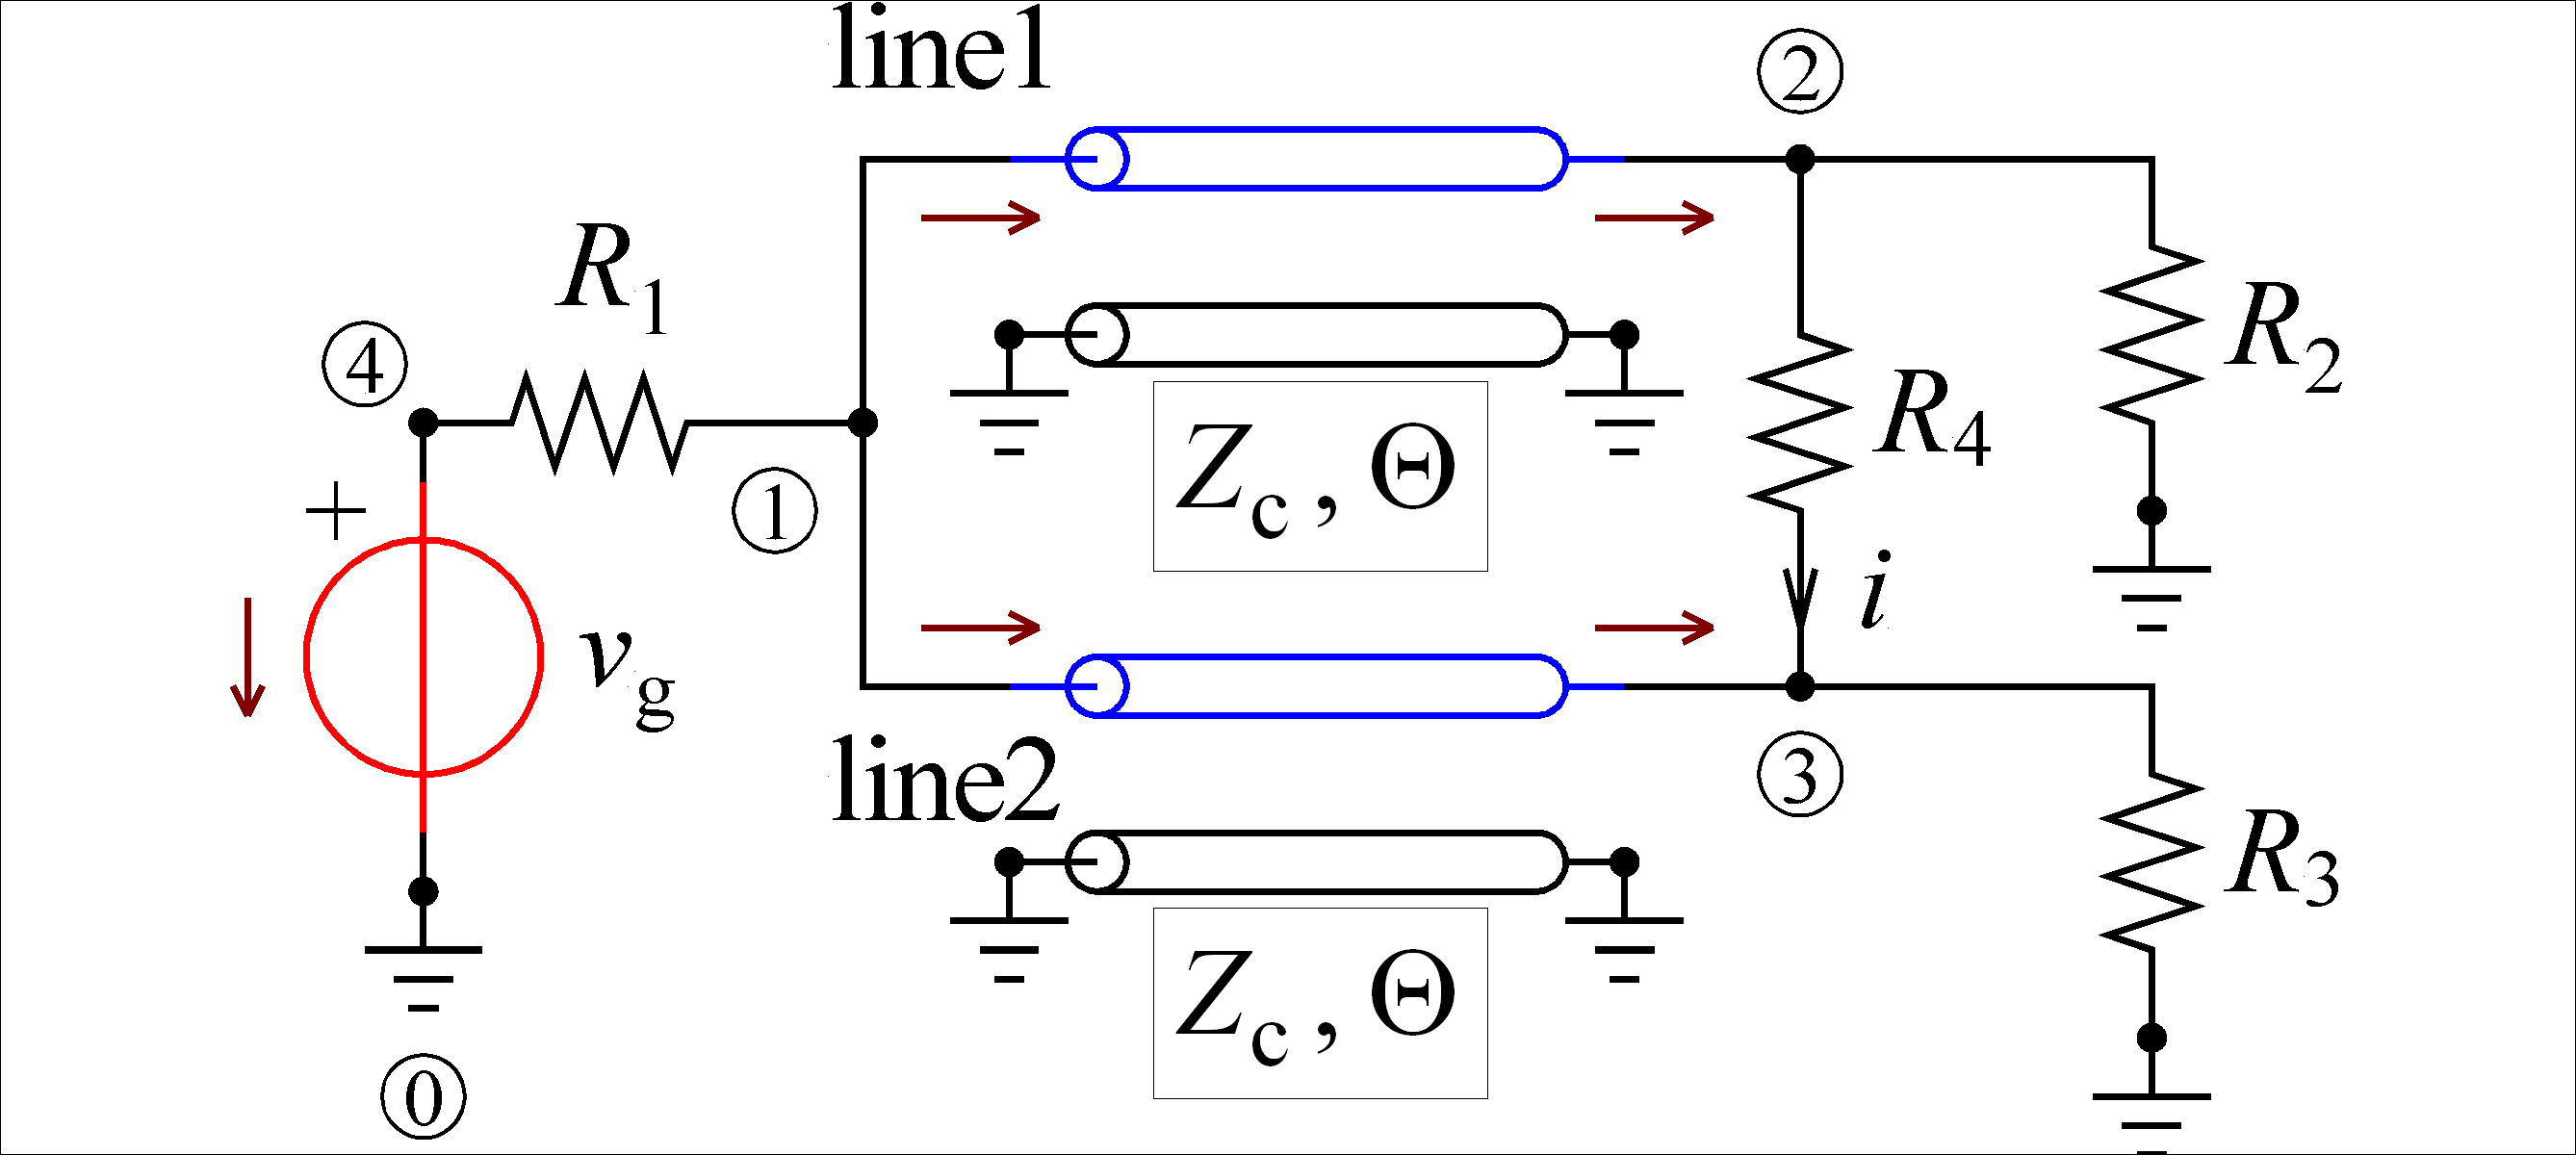
\includegraphics[scale = 0.65]{Figure6.png}\\
       Figure 6: Wilkinson power divider.
   \end{center} 
    

    \textbf{Step 5.1.} Repeat steps 1.2.-1.7.

    \begin{tcolorbox}[breakable, size=fbox, boxrule=1pt, pad at break*=1mm,colback=cellbackground, colframe=cellborder]
\prompt{In}{incolor}{36}{\boxspacing}
\begin{Verbatim}[commandchars=\\\{\}]
\PY{k+kn}{from} \PY{n+nn}{symPyCAP} \PY{k+kn}{import} \PY{n}{Circuit}
\PY{k+kn}{import} \PY{n+nn}{sympy}
\end{Verbatim}
\end{tcolorbox}

    \begin{tcolorbox}[breakable, size=fbox, boxrule=1pt, pad at break*=1mm,colback=cellbackground, colframe=cellborder]
\prompt{In}{incolor}{37}{\boxspacing}
\begin{Verbatim}[commandchars=\\\{\}]
\PY{n}{R} \PY{o}{=} \PY{n}{Symbol}\PY{p}{(}\PY{l+s+s1}{\PYZsq{}}\PY{l+s+s1}{R}\PY{l+s+s1}{\PYZsq{}}\PY{p}{)}
\PY{n}{W} \PY{o}{=} \PY{n}{symbols}\PY{p}{(}\PY{l+s+s1}{\PYZsq{}}\PY{l+s+s1}{W}\PY{l+s+s1}{\PYZsq{}}\PY{p}{)}
\end{Verbatim}
\end{tcolorbox}

    \textbf{Note:} {\setlength{\fboxsep}{2pt}\colorbox{LightGray}{\texttt{sympy.sqrt()}}} and {\setlength{\fboxsep}{2pt}\colorbox{LightGray}{\texttt{sympy.pi}}} should be
used, not {\setlength{\fboxsep}{2pt}\colorbox{LightGray}{\texttt{math.sqrt()}}} and {\setlength{\fboxsep}{2pt}\colorbox{LightGray}{\texttt{math.pi}}}.

    \begin{tcolorbox}[breakable, size=fbox, boxrule=1pt, pad at break*=1mm,colback=cellbackground, colframe=cellborder]
\prompt{In}{incolor}{38}{\boxspacing}
\begin{Verbatim}[commandchars=\\\{\}]
\PY{n}{Wilkinson\PYZus{}schematic} \PY{o}{=} \PY{p}{[}
    \PY{p}{[}\PY{l+s+s2}{\PYZdq{}}\PY{l+s+s2}{V}\PY{l+s+s2}{\PYZdq{}}\PY{p}{,} \PY{l+s+s2}{\PYZdq{}}\PY{l+s+s2}{Vg}\PY{l+s+s2}{\PYZdq{}}\PY{p}{,} \PY{l+m+mi}{4}\PY{p}{,} \PY{l+m+mi}{0}\PY{p}{]}\PY{p}{,}
    \PY{p}{[}\PY{l+s+s2}{\PYZdq{}}\PY{l+s+s2}{R}\PY{l+s+s2}{\PYZdq{}}\PY{p}{,} \PY{l+s+s2}{\PYZdq{}}\PY{l+s+s2}{R1}\PY{l+s+s2}{\PYZdq{}}\PY{p}{,} \PY{l+m+mi}{1}\PY{p}{,} \PY{l+m+mi}{4}\PY{p}{]}\PY{p}{,}
    \PY{p}{[}\PY{l+s+s2}{\PYZdq{}}\PY{l+s+s2}{R}\PY{l+s+s2}{\PYZdq{}}\PY{p}{,} \PY{l+s+s2}{\PYZdq{}}\PY{l+s+s2}{R2}\PY{l+s+s2}{\PYZdq{}}\PY{p}{,} \PY{l+m+mi}{2}\PY{p}{,} \PY{l+m+mi}{0}\PY{p}{]}\PY{p}{,}
    \PY{p}{[}\PY{l+s+s2}{\PYZdq{}}\PY{l+s+s2}{R}\PY{l+s+s2}{\PYZdq{}}\PY{p}{,} \PY{l+s+s2}{\PYZdq{}}\PY{l+s+s2}{R3}\PY{l+s+s2}{\PYZdq{}}\PY{p}{,} \PY{l+m+mi}{3}\PY{p}{,} \PY{l+m+mi}{0}\PY{p}{]}\PY{p}{,}
    \PY{p}{[}\PY{l+s+s2}{\PYZdq{}}\PY{l+s+s2}{R}\PY{l+s+s2}{\PYZdq{}}\PY{p}{,} \PY{l+s+s2}{\PYZdq{}}\PY{l+s+s2}{R4}\PY{l+s+s2}{\PYZdq{}}\PY{p}{,} \PY{l+m+mi}{2}\PY{p}{,} \PY{l+m+mi}{3}\PY{p}{]}\PY{p}{,}
    \PY{p}{[}\PY{l+s+s2}{\PYZdq{}}\PY{l+s+s2}{T}\PY{l+s+s2}{\PYZdq{}}\PY{p}{,} \PY{l+s+s2}{\PYZdq{}}\PY{l+s+s2}{T1}\PY{l+s+s2}{\PYZdq{}}\PY{p}{,} \PY{p}{[}\PY{l+m+mi}{1}\PY{p}{,}\PY{l+m+mi}{0}\PY{p}{]}\PY{p}{,} \PY{p}{[}\PY{l+m+mi}{2}\PY{p}{,}\PY{l+m+mi}{0}\PY{p}{]}\PY{p}{,} \PY{p}{[}\PY{n}{sympy}\PY{o}{.}\PY{n}{sqrt}\PY{p}{(}\PY{l+m+mi}{2}\PY{p}{)}\PY{o}{*}\PY{n}{R}\PY{p}{,}\PY{n}{sympy}\PY{o}{.}\PY{n}{pi}\PY{o}{/}\PY{l+m+mi}{2}\PY{p}{]}\PY{p}{]}\PY{p}{,}
    \PY{p}{[}\PY{l+s+s2}{\PYZdq{}}\PY{l+s+s2}{T}\PY{l+s+s2}{\PYZdq{}}\PY{p}{,} \PY{l+s+s2}{\PYZdq{}}\PY{l+s+s2}{T2}\PY{l+s+s2}{\PYZdq{}}\PY{p}{,} \PY{p}{[}\PY{l+m+mi}{1}\PY{p}{,}\PY{l+m+mi}{0}\PY{p}{]}\PY{p}{,} \PY{p}{[}\PY{l+m+mi}{3}\PY{p}{,}\PY{l+m+mi}{0}\PY{p}{]}\PY{p}{,} \PY{p}{[}\PY{n}{sympy}\PY{o}{.}\PY{n}{sqrt}\PY{p}{(}\PY{l+m+mi}{2}\PY{p}{)}\PY{o}{*}\PY{n}{R}\PY{p}{,}\PY{n}{sympy}\PY{o}{.}\PY{n}{pi}\PY{o}{/}\PY{l+m+mi}{2}\PY{p}{]}\PY{p}{]}
\PY{p}{]}
\end{Verbatim}
\end{tcolorbox}

    \begin{tcolorbox}[breakable, size=fbox, boxrule=1pt, pad at break*=1mm,colback=cellbackground, colframe=cellborder]
\prompt{In}{incolor}{39}{\boxspacing}
\begin{Verbatim}[commandchars=\\\{\}]
\PY{n}{Wilkinson_circuit} \PY{o}{=} \PY{n}{Circuit}\PY{p}{(}\PY{n}{Wilkinson\PYZus{}schematic}\PY{p}{)}
\end{Verbatim}
\end{tcolorbox}

    \begin{tcolorbox}[breakable, size=fbox, boxrule=1pt, pad at break*=1mm,colback=cellbackground, colframe=cellborder]
\prompt{In}{incolor}{40}{\boxspacing}
\begin{Verbatim}[commandchars=\\\{\}]
\PY{n}{Wilkinson_circuit}\PY{o}{.}\PY{n}{symPyCAP}\PY{p}{(}\PY{n}{w} \PY{o}{=} \PY{n}{W}\PY{p}{,} \PY{n}{replacement} \PY{o}{=} \PY{p}{\PYZob{}}\PY{l+s+s2}{\PYZdq{}}\PY{l+s+s2}{R1}\PY{l+s+s2}{\PYZdq{}} \PY{p}{:} \PY{n}{R}\PY{p}{,} \PY{l+s+s2}{\PYZdq{}}\PY{l+s+s2}{R2}\PY{l+s+s2}{\PYZdq{}} \PY{p}{:} \PY{n}{R}\PY{p}{,} \PY{l+s+s2}{\PYZdq{}}\PY{l+s+s2}{R3}\PY{l+s+s2}{\PYZdq{}} \PY{p}{:} \PY{n}{R}\PY{p}{,} \PY{l+s+s2}{\PYZdq{}}\PY{l+s+s2}{R4}\PY{l+s+s2}{\PYZdq{}} \PY{p}{:} \PY{l+m+mi}{2}\PY{o}{*}\PY{n}{R}\PY{p}{\PYZcb{}}\PY{p}{)} 
\end{Verbatim}
\end{tcolorbox}

    \begin{tcolorbox}[breakable, size=fbox, boxrule=1pt, pad at break*=1mm,colback=cellbackground, colframe=cellborder]
\prompt{In}{incolor}{41}{\boxspacing}
\begin{Verbatim}[commandchars=\\\{\}]
\PY{n}{Wilkinson_circuit}\PY{o}{.}\PY{n}{print\PYZus{}specific\PYZus{}solutions}\PY{p}{(}\PY{p}{)}
\end{Verbatim}
\end{tcolorbox}

    \begin{Verbatim}[commandchars=\\\{\}]
V1 : Vg/2

V2 : -sqrt(2)*I*Vg/4

V3 : -sqrt(2)*I*Vg/4

V4 : Vg

IVg : -Vg/(2*R)

IT1\_1 : Vg/(4*R)

IT1\_2 : -sqrt(2)*I*Vg/(4*R)

IT2\_1 : Vg/(4*R)

IT2\_3 : -sqrt(2)*I*Vg/(4*R)

    \end{Verbatim}
    
    \textbf{Note:} \textbf{\textit{I}} represents the imaginary unit in Python, \textbf{\textit{I = $\sqrt{-1}$}}. It is not the current at a port of an element.

    \textbf{Step 5.2.} Compare the voltages of the \(2^{nd}\) and \(3^{rd}\)
node.

    \begin{tcolorbox}[breakable, size=fbox, boxrule=1pt, pad at break*=1mm,colback=cellbackground, colframe=cellborder]
\prompt{In}{incolor}{42}{\boxspacing}
\begin{Verbatim}[commandchars=\\\{\}]
\PY{n}{simplify}\PY{p}{(}\PY{n}{Wilkinson_circuit}\PY{o}{.}\PY{n}{get\PYZus{}specific\PYZus{}solutions}\PY{p}{(}\PY{p}{)}\PY{p}{[}\PY{l+s+s1}{\PYZsq{}}\PY{l+s+s1}{V2}\PY{l+s+s1}{\PYZsq{}}\PY{p}{]}\PY{o}{\PYZhy{}}\PY{n}{Wilkinson_circuit}\PY{o}{.}\PY{n}{get\PYZus{}specific\PYZus{}solutions}\PY{p}{(}\PY{p}{)}\PY{p}{[}\PY{l+s+s1}{\PYZsq{}}\PY{l+s+s1}{V3}\PY{l+s+s1}{\PYZsq{}}\PY{p}{]}\PY{p}{)} \PY{o}{==} \PY{l+m+mi}{0}
\end{Verbatim}
\end{tcolorbox}

            \begin{tcolorbox}[breakable, size=fbox, boxrule=.5pt, pad at break*=1mm, opacityfill=0]
\prompt{Out}{outcolor}{42}{\boxspacing}
\begin{Verbatim}[commandchars=\\\{\}]
True
\end{Verbatim}
\end{tcolorbox}
        
    \begin{center}\rule{0.5\linewidth}{0.5pt}\end{center}

    \hypertarget{example-6-transmission-line-circuit}{%
\section*{\texorpdfstring{Example 6: Transmission line circuit
}{Example 6: Transmission line circuit }}\label{example6}}

Doubly terminated lossless transmission line section is shown in Figure 7.
The corresponding symbolic analysis, performed in the \textbf{\textit{s}}-domain, verifies
that the circuit acts as a delay line.

    \begin{center}
   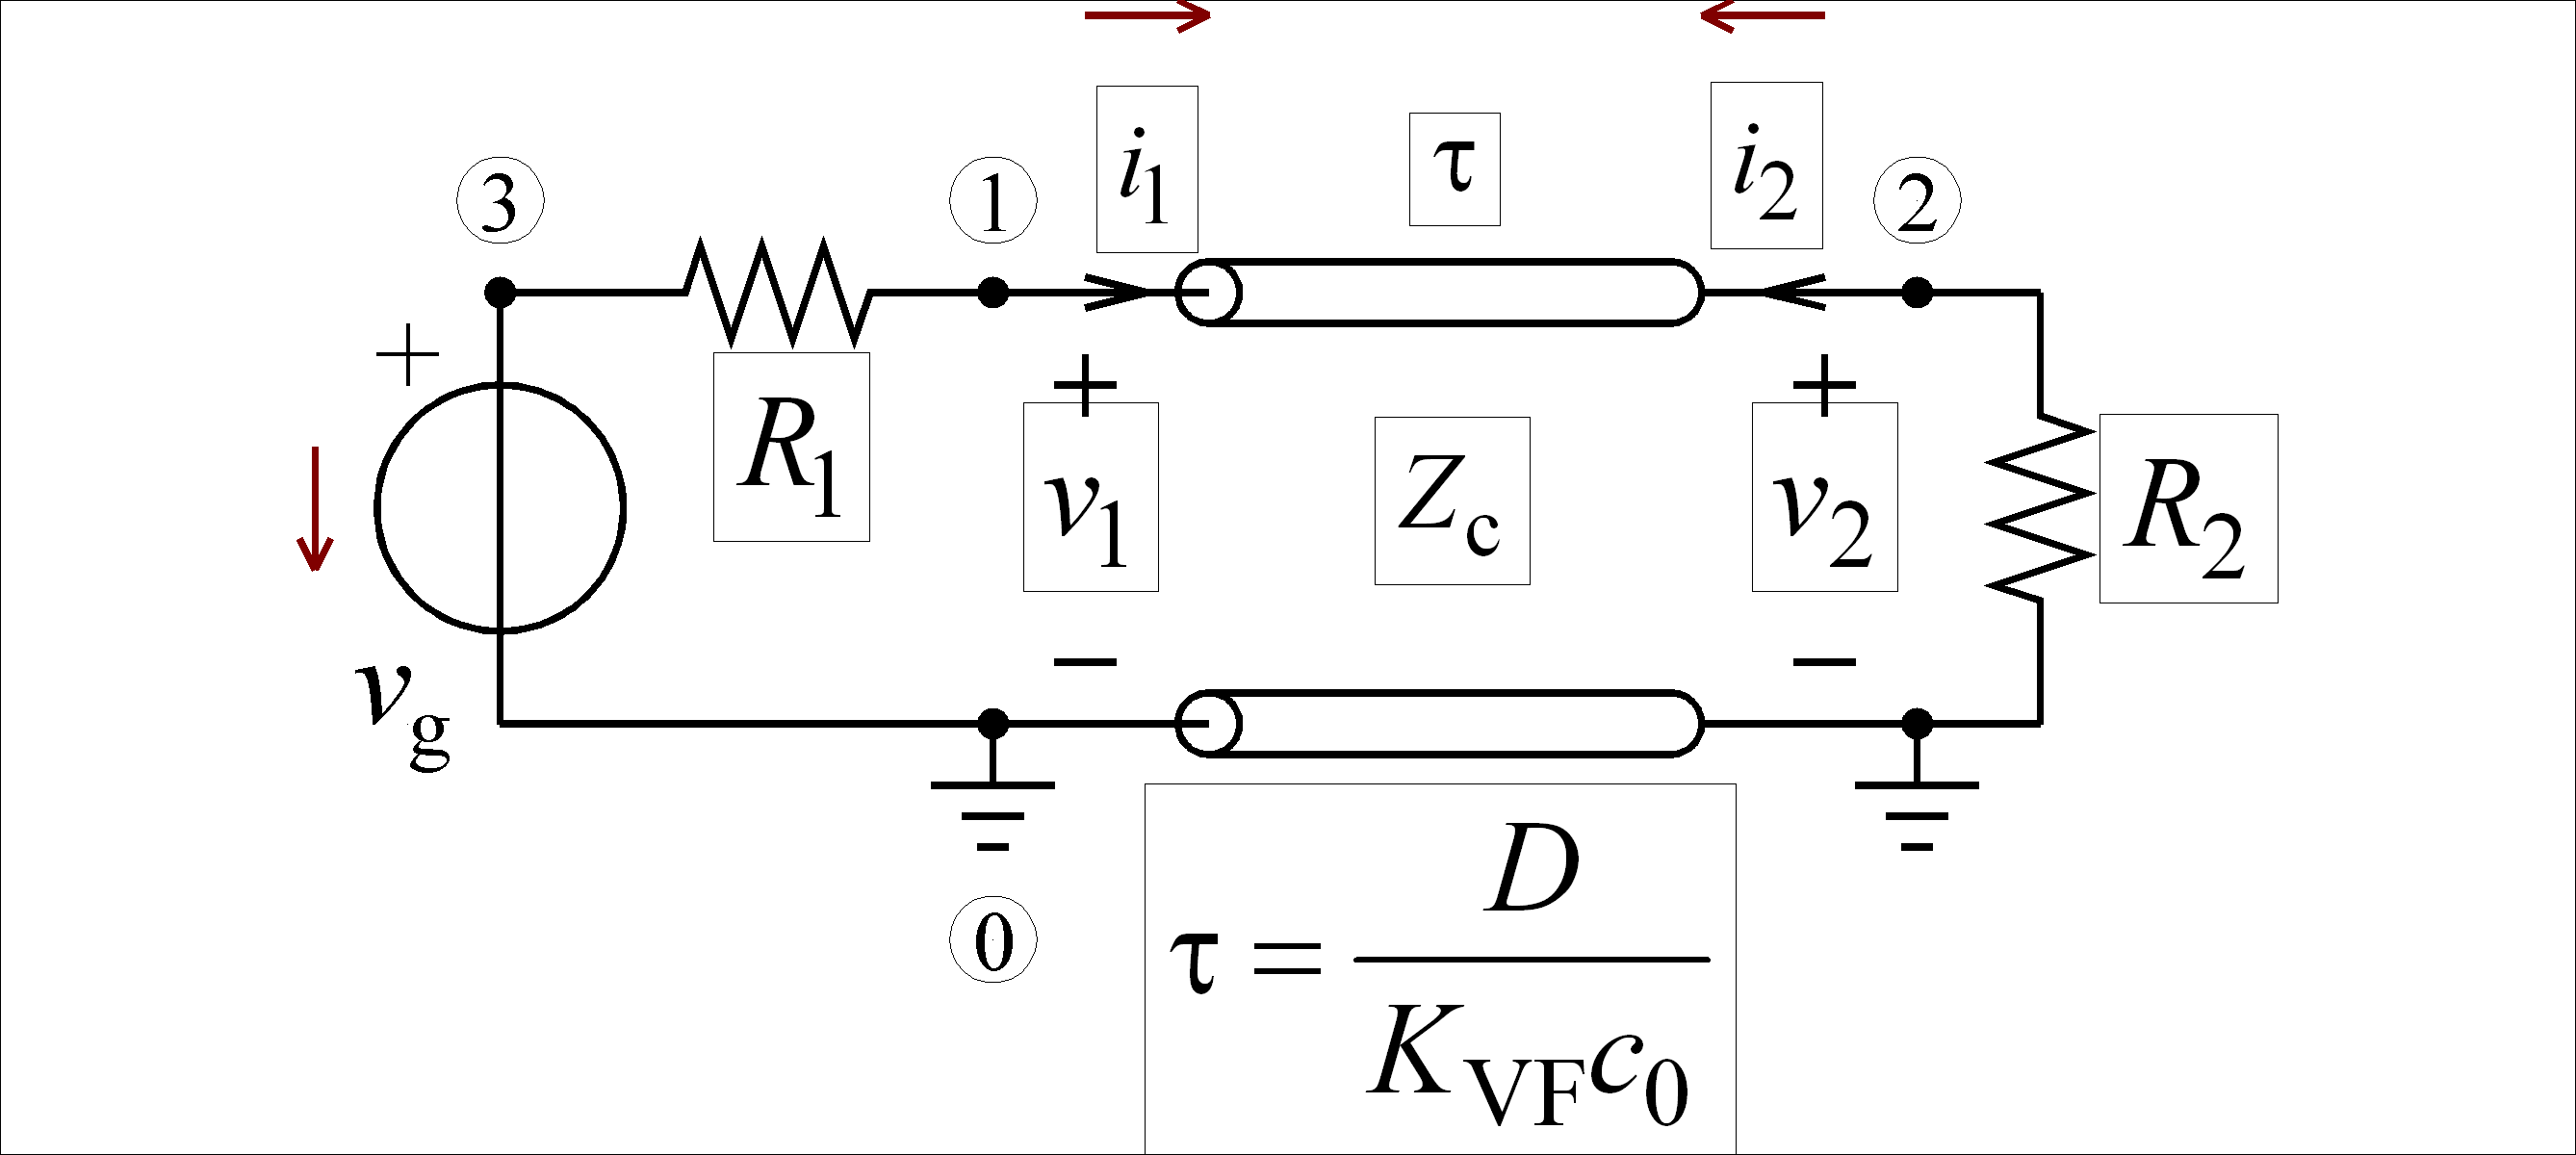
\includegraphics[scale = 0.65]{Figure7.png}\\
       Figure 7: Transmission line circuit; the \textbf{\textit{s}}-domain.
   \end{center} 
    

    \textbf{Step 6.1.} Repeat steps 1.2.-1.7.

    \begin{tcolorbox}[breakable, size=fbox, boxrule=1pt, pad at break*=1mm,colback=cellbackground, colframe=cellborder]
\prompt{In}{incolor}{43}{\boxspacing}
\begin{Verbatim}[commandchars=\\\{\}]
\PY{k+kn}{from} \PY{n+nn}{symPyCAP} \PY{k+kn}{import} \PY{n}{Circuit}
\PY{k+kn}{from} \PY{n+nn}{sympy} \PY{k+kn}{import} \PY{o}{*}
\end{Verbatim}
\end{tcolorbox}

    \begin{tcolorbox}[breakable, size=fbox, boxrule=1pt, pad at break*=1mm,colback=cellbackground, colframe=cellborder]
\prompt{In}{incolor}{44}{\boxspacing}
\begin{Verbatim}[commandchars=\\\{\}]
\PY{n}{Zc} \PY{o}{=} \PY{n}{Symbol}\PY{p}{(}\PY{l+s+s1}{\PYZsq{}}\PY{l+s+s1}{Zc}\PY{l+s+s1}{\PYZsq{}}\PY{p}{)}
\PY{n}{tau} \PY{o}{=} \PY{n}{symbols}\PY{p}{(}\PY{l+s+sa}{r}\PY{l+s+s1}{\PYZsq{}}\PY{l+s+s1}{tau}\PY{l+s+s1}{\PYZsq{}}\PY{p}{)}
\end{Verbatim}
\end{tcolorbox}

    \begin{tcolorbox}[breakable, size=fbox, boxrule=1pt, pad at break*=1mm,colback=cellbackground, colframe=cellborder]
\prompt{In}{incolor}{45}{\boxspacing}
\begin{Verbatim}[commandchars=\\\{\}]
\PY{n}{TLine\PYZus{}schematic} \PY{o}{=} \PY{p}{[}
    \PY{p}{[}\PY{l+s+s2}{\PYZdq{}}\PY{l+s+s2}{V}\PY{l+s+s2}{\PYZdq{}}\PY{p}{,} \PY{l+s+s2}{\PYZdq{}}\PY{l+s+s2}{Vg}\PY{l+s+s2}{\PYZdq{}}\PY{p}{,} \PY{l+m+mi}{3}\PY{p}{,} \PY{l+m+mi}{0}\PY{p}{]}\PY{p}{,}
    \PY{p}{[}\PY{l+s+s2}{\PYZdq{}}\PY{l+s+s2}{R}\PY{l+s+s2}{\PYZdq{}}\PY{p}{,} \PY{l+s+s2}{\PYZdq{}}\PY{l+s+s2}{R1}\PY{l+s+s2}{\PYZdq{}}\PY{p}{,} \PY{l+m+mi}{3}\PY{p}{,} \PY{l+m+mi}{1}\PY{p}{]}\PY{p}{,}
    \PY{p}{[}\PY{l+s+s2}{\PYZdq{}}\PY{l+s+s2}{T}\PY{l+s+s2}{\PYZdq{}}\PY{p}{,} \PY{l+s+s2}{\PYZdq{}}\PY{l+s+s2}{T1}\PY{l+s+s2}{\PYZdq{}}\PY{p}{,} \PY{p}{[}\PY{l+m+mi}{1}\PY{p}{,}\PY{l+m+mi}{0}\PY{p}{]}\PY{p}{,} \PY{p}{[}\PY{l+m+mi}{2}\PY{p}{,}\PY{l+m+mi}{0}\PY{p}{]}\PY{p}{,} \PY{p}{[}\PY{n}{Zc}\PY{p}{,}\PY{n}{tau}\PY{p}{]}\PY{p}{]}\PY{p}{,}
    \PY{p}{[}\PY{l+s+s2}{\PYZdq{}}\PY{l+s+s2}{R}\PY{l+s+s2}{\PYZdq{}}\PY{p}{,} \PY{l+s+s2}{\PYZdq{}}\PY{l+s+s2}{R2}\PY{l+s+s2}{\PYZdq{}}\PY{p}{,} \PY{l+m+mi}{2}\PY{p}{,} \PY{l+m+mi}{0}\PY{p}{]}
\PY{p}{]}
\end{Verbatim}
\end{tcolorbox}

    \begin{tcolorbox}[breakable, size=fbox, boxrule=1pt, pad at break*=1mm,colback=cellbackground, colframe=cellborder]
\prompt{In}{incolor}{46}{\boxspacing}
\begin{Verbatim}[commandchars=\\\{\}]
\PY{n}{TLine_circuit} \PY{o}{=} \PY{n}{Circuit}\PY{p}{(}\PY{n}{TLine\PYZus{}schematic}\PY{p}{)}
\end{Verbatim}
\end{tcolorbox}

    \begin{tcolorbox}[breakable, size=fbox, boxrule=1pt, pad at break*=1mm,colback=cellbackground, colframe=cellborder]
\prompt{In}{incolor}{47}{\boxspacing}
\begin{Verbatim}[commandchars=\\\{\}]
\PY{n}{TLine_circuit}\PY{o}{.}\PY{n}{symPyCAP}\PY{p}{(}\PY{n}{replacement} \PY{o}{=} \PY{p}{\PYZob{}}\PY{l+s+s2}{\PYZdq{}}\PY{l+s+s2}{R1}\PY{l+s+s2}{\PYZdq{}} \PY{p}{:} \PY{n}{Zc}\PY{p}{,} \PY{l+s+s2}{\PYZdq{}}\PY{l+s+s2}{R2}\PY{l+s+s2}{\PYZdq{}} \PY{p}{:} \PY{n}{Zc}\PY{p}{\PYZcb{}}\PY{p}{)} 
\end{Verbatim}
\end{tcolorbox}

    \begin{tcolorbox}[breakable, size=fbox, boxrule=1pt, pad at break*=1mm,colback=cellbackground, colframe=cellborder]
\prompt{In}{incolor}{48}{\boxspacing}
\begin{Verbatim}[commandchars=\\\{\}]
\PY{n}{TLine_circuit}\PY{o}{.}\PY{n}{print\PYZus{}specific\PYZus{}solutions}\PY{p}{(}\PY{p}{)}
\end{Verbatim}
\end{tcolorbox}

    \begin{Verbatim}[commandchars=\\\{\}]
V1 : Vg/2

V2 : Vg*exp(-s*tau)/2

V3 : Vg

IVg : -Vg/(2*Zc)

IT1\_1 : Vg/(2*Zc)

IT1\_2 : -Vg*exp(-s*tau)/(2*Zc)

    \end{Verbatim}

    \begin{tcolorbox}[breakable, size=fbox, boxrule=1pt, pad at break*=1mm,colback=cellbackground, colframe=cellborder]
\prompt{In}{incolor}{49}{\boxspacing}
\begin{Verbatim}[commandchars=\\\{\}]
\PY{n}{TLine_circuit}\PY{o}{.}\PY{n}{get\PYZus{}specific\PYZus{}solutions}\PY{p}{(}\PY{p}{)}\PY{p}{[}\PY{l+s+s2}{\PYZdq{}}\PY{l+s+s2}{V2}\PY{l+s+s2}{\PYZdq{}}\PY{p}{]}
\end{Verbatim}
\end{tcolorbox}
 
            
\prompt{Out}{outcolor}{49}{}
    
    $\displaystyle \frac{Vg e^{- s \tau}}{2}$

    

    \begin{center}\rule{0.5\linewidth}{0.5pt}\end{center}

    \hypertarget{example-7-adder}{%
\section*{\texorpdfstring{Example 7: Adder
}{Example 7: Adder }}\label{example7}}

Adder, which is realized an with operational amplifier, is shown in
Figure 8. The sum of all generator voltages should be obtained at the
output of the operational amplifier.

    \begin{center}
   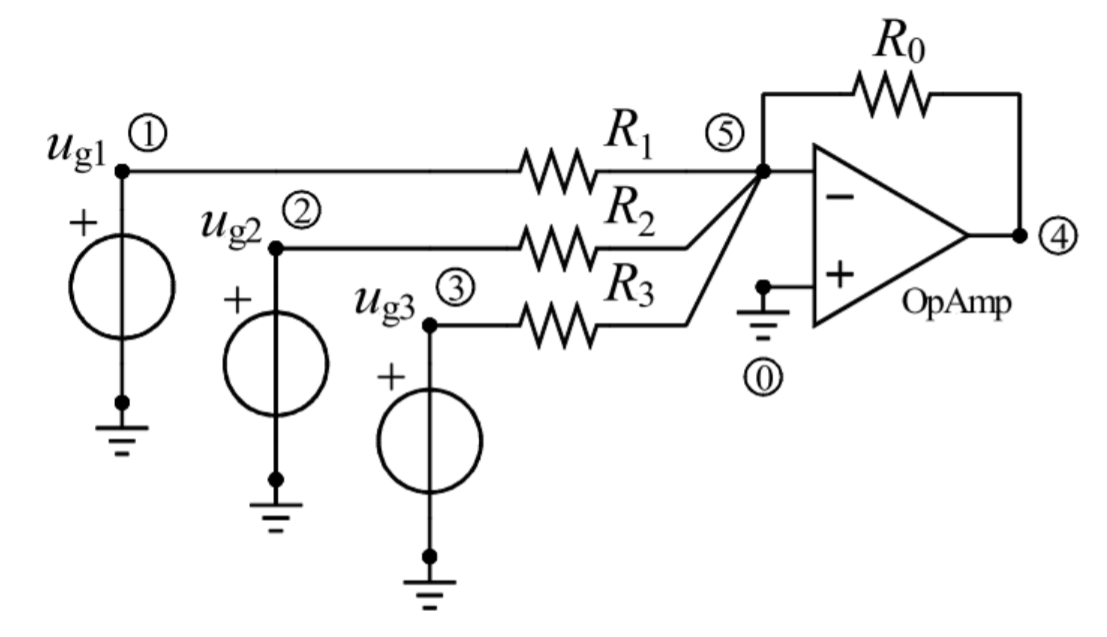
\includegraphics[scale = 0.6]{Figure8.png}\\
        Figure 8: Adder.
   \end{center} 
   

    \textbf{Step 7.1.} Repeat steps 1.2-1.7.

    \begin{tcolorbox}[breakable, size=fbox, boxrule=1pt, pad at break*=1mm,colback=cellbackground, colframe=cellborder]
\prompt{In}{incolor}{50}{\boxspacing}
\begin{Verbatim}[commandchars=\\\{\}]
\PY{k+kn}{from} \PY{n+nn}{symPyCAP} \PY{k+kn}{import} \PY{n}{Circuit}
\PY{k+kn}{import} \PY{n+nn}{sympy}
\end{Verbatim}
\end{tcolorbox}

    \begin{tcolorbox}[breakable, size=fbox, boxrule=1pt, pad at break*=1mm,colback=cellbackground, colframe=cellborder]
\prompt{In}{incolor}{51}{\boxspacing}
\begin{Verbatim}[commandchars=\\\{\}]
\PY{n}{R} \PY{o}{=} \PY{n}{sympy}\PY{o}{.}\PY{n}{Symbol}\PY{p}{(}\PY{l+s+s1}{\PYZsq{}}\PY{l+s+s1}{R}\PY{l+s+s1}{\PYZsq{}}\PY{p}{)}
\PY{n}{Ug1} \PY{o}{=} \PY{n}{sympy}\PY{o}{.}\PY{n}{Symbol}\PY{p}{(}\PY{l+s+s1}{\PYZsq{}}\PY{l+s+s1}{Ug1}\PY{l+s+s1}{\PYZsq{}}\PY{p}{)}
\PY{n}{Ug2} \PY{o}{=} \PY{n}{sympy}\PY{o}{.}\PY{n}{Symbol}\PY{p}{(}\PY{l+s+s1}{\PYZsq{}}\PY{l+s+s1}{Ug2}\PY{l+s+s1}{\PYZsq{}}\PY{p}{)}
\PY{n}{Ug3} \PY{o}{=} \PY{n}{sympy}\PY{o}{.}\PY{n}{Symbol}\PY{p}{(}\PY{l+s+s1}{\PYZsq{}}\PY{l+s+s1}{Ug3}\PY{l+s+s1}{\PYZsq{}}\PY{p}{)}
\end{Verbatim}
\end{tcolorbox}

    \begin{tcolorbox}[breakable, size=fbox, boxrule=1pt, pad at break*=1mm,colback=cellbackground, colframe=cellborder]
\prompt{In}{incolor}{52}{\boxspacing}
\begin{Verbatim}[commandchars=\\\{\}]
\PY{n}{Adder\PYZus{}schematic} \PY{o}{=} \PY{p}{[}
    \PY{p}{[}\PY{l+s+s2}{\PYZdq{}}\PY{l+s+s2}{R}\PY{l+s+s2}{\PYZdq{}}\PY{p}{,} \PY{l+s+s2}{\PYZdq{}}\PY{l+s+s2}{R1}\PY{l+s+s2}{\PYZdq{}}\PY{p}{,} \PY{l+m+mi}{5}\PY{p}{,} \PY{l+m+mi}{1}\PY{p}{]}\PY{p}{,}
    \PY{p}{[}\PY{l+s+s2}{\PYZdq{}}\PY{l+s+s2}{R}\PY{l+s+s2}{\PYZdq{}}\PY{p}{,} \PY{l+s+s2}{\PYZdq{}}\PY{l+s+s2}{R2}\PY{l+s+s2}{\PYZdq{}}\PY{p}{,} \PY{l+m+mi}{5}\PY{p}{,} \PY{l+m+mi}{2}\PY{p}{]}\PY{p}{,}
    \PY{p}{[}\PY{l+s+s2}{\PYZdq{}}\PY{l+s+s2}{R}\PY{l+s+s2}{\PYZdq{}}\PY{p}{,} \PY{l+s+s2}{\PYZdq{}}\PY{l+s+s2}{R3}\PY{l+s+s2}{\PYZdq{}}\PY{p}{,} \PY{l+m+mi}{5}\PY{p}{,} \PY{l+m+mi}{3}\PY{p}{]}\PY{p}{,}
    \PY{p}{[}\PY{l+s+s2}{\PYZdq{}}\PY{l+s+s2}{R}\PY{l+s+s2}{\PYZdq{}}\PY{p}{,} \PY{l+s+s2}{\PYZdq{}}\PY{l+s+s2}{R0}\PY{l+s+s2}{\PYZdq{}}\PY{p}{,} \PY{l+m+mi}{5}\PY{p}{,} \PY{l+m+mi}{4}\PY{p}{]}\PY{p}{,}
    \PY{p}{[}\PY{l+s+s2}{\PYZdq{}}\PY{l+s+s2}{V}\PY{l+s+s2}{\PYZdq{}}\PY{p}{,} \PY{l+s+s2}{\PYZdq{}}\PY{l+s+s2}{Vg1}\PY{l+s+s2}{\PYZdq{}}\PY{p}{,} \PY{l+m+mi}{1}\PY{p}{,} \PY{l+m+mi}{0}\PY{p}{]}\PY{p}{,}
    \PY{p}{[}\PY{l+s+s2}{\PYZdq{}}\PY{l+s+s2}{V}\PY{l+s+s2}{\PYZdq{}}\PY{p}{,} \PY{l+s+s2}{\PYZdq{}}\PY{l+s+s2}{Vg2}\PY{l+s+s2}{\PYZdq{}}\PY{p}{,} \PY{l+m+mi}{2}\PY{p}{,} \PY{l+m+mi}{0}\PY{p}{]}\PY{p}{,}
    \PY{p}{[}\PY{l+s+s2}{\PYZdq{}}\PY{l+s+s2}{V}\PY{l+s+s2}{\PYZdq{}}\PY{p}{,} \PY{l+s+s2}{\PYZdq{}}\PY{l+s+s2}{Vg3}\PY{l+s+s2}{\PYZdq{}}\PY{p}{,} \PY{l+m+mi}{3}\PY{p}{,} \PY{l+m+mi}{0}\PY{p}{]}\PY{p}{,}
    \PY{p}{[}\PY{l+s+s2}{\PYZdq{}}\PY{l+s+s2}{OpAmp}\PY{l+s+s2}{\PYZdq{}}\PY{p}{,} \PY{l+s+s2}{\PYZdq{}}\PY{l+s+s2}{OpAmp1}\PY{l+s+s2}{\PYZdq{}}\PY{p}{,} \PY{p}{[}\PY{l+m+mi}{0}\PY{p}{,}\PY{l+m+mi}{5}\PY{p}{]}\PY{p}{,} \PY{l+m+mi}{4}\PY{p}{]}
\PY{p}{]}
\end{Verbatim}
\end{tcolorbox}

    \begin{tcolorbox}[breakable, size=fbox, boxrule=1pt, pad at break*=1mm,colback=cellbackground, colframe=cellborder]
\prompt{In}{incolor}{53}{\boxspacing}
\begin{Verbatim}[commandchars=\\\{\}]
\PY{n}{Adder_circuit} \PY{o}{=} \PY{n}{Circuit}\PY{p}{(}\PY{n}{Adder\PYZus{}schematic}\PY{p}{)}
\end{Verbatim}
\end{tcolorbox}

    \begin{tcolorbox}[breakable, size=fbox, boxrule=1pt, pad at break*=1mm,colback=cellbackground, colframe=cellborder]
\prompt{In}{incolor}{54}{\boxspacing}
\begin{Verbatim}[commandchars=\\\{\}]
\PY{n}{Adder_circuit}\PY{o}{.}\PY{n}{symPyCAP}\PY{p}{(}\PY{n}{replacement} \PY{o}{=} \PY{p}{\PYZob{}}\PY{l+s+s2}{\PYZdq{}}\PY{l+s+s2}{R1}\PY{l+s+s2}{\PYZdq{}} \PY{p}{:} \PY{n}{R}\PY{p}{,} \PY{l+s+s2}{\PYZdq{}}\PY{l+s+s2}{R2}\PY{l+s+s2}{\PYZdq{}} \PY{p}{:} \PY{n}{R}\PY{p}{,} \PY{l+s+s2}{\PYZdq{}}\PY{l+s+s2}{R3}\PY{l+s+s2}{\PYZdq{}} \PY{p}{:} \PY{n}{R}\PY{p}{,} \PY{l+s+s2}{\PYZdq{}}\PY{l+s+s2}{R0}\PY{l+s+s2}{\PYZdq{}} \PY{p}{:} \PY{n}{R}\PY{p}{,} \PY{l+s+s2}{\PYZdq{}}\PY{l+s+s2}{Vg1}\PY{l+s+s2}{\PYZdq{}} \PY{p}{:} \PY{n}{Ug1}\PY{p}{,} \PY{l+s+s2}{\PYZdq{}}\PY{l+s+s2}{Vg2}\PY{l+s+s2}{\PYZdq{}} \PY{p}{:} \PY{n}{Ug2}\PY{p}{,} \PY{l+s+s2}{\PYZdq{}}\PY{l+s+s2}{Vg3}\PY{l+s+s2}{\PYZdq{}} \PY{p}{:} \PY{n}{Ug3}\PY{p}{\PYZcb{}}\PY{p}{)} 
\end{Verbatim}
\end{tcolorbox}

    \begin{tcolorbox}[breakable, size=fbox, boxrule=1pt, pad at break*=1mm,colback=cellbackground, colframe=cellborder]
\prompt{In}{incolor}{55}{\boxspacing}
\begin{Verbatim}[commandchars=\\\{\}]
\PY{n}{Adder_circuit}\PY{o}{.}\PY{n}{print\PYZus{}specific\PYZus{}solutions}\PY{p}{(}\PY{p}{)}
\end{Verbatim}
\end{tcolorbox}

    \begin{Verbatim}[commandchars=\\\{\}]
V1 : Ug1

V2 : Ug2

V3 : Ug3

V4 : -Ug1 - Ug2 - Ug3

V5 : 0

IVg1 : -Ug1/R

IVg2 : -Ug2/R

IVg3 : -Ug3/R

IOpAmp1 : (Ug1 + Ug2 + Ug3)/R

    \end{Verbatim}

    \begin{center}\rule{0.5\linewidth}{0.5pt}\end{center}

    \hypertarget{example-8-subtractor}{%
\section*{\texorpdfstring{Example 8: Subtractor
}{Example 8: Subtractor }}\label{example8}}

Subtractor, which is realized with an operational amplifier, is shown in
Figure 9.

    \begin{center}
   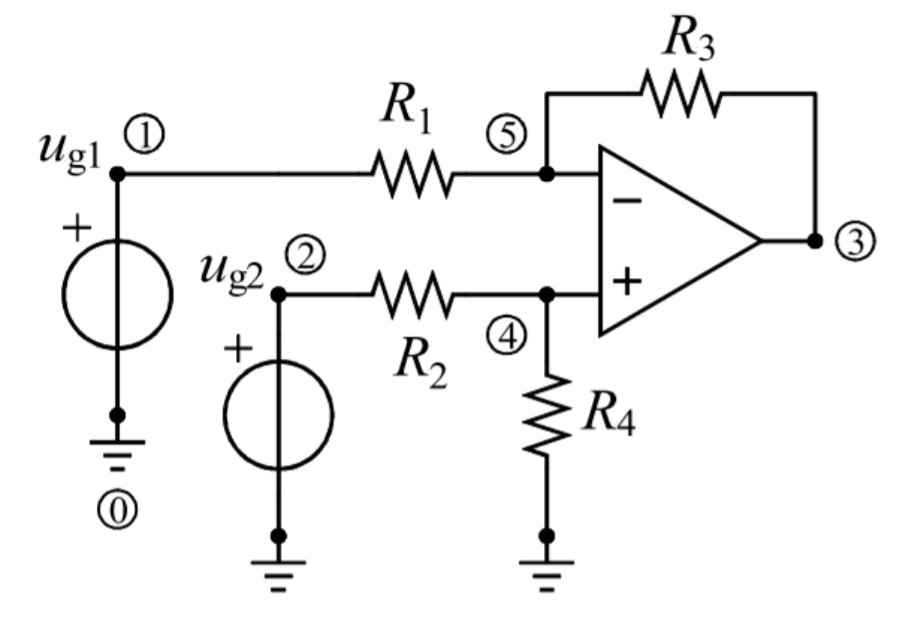
\includegraphics[scale = 0.5]{Figure9.png}\\
       Figure 9: Subtractor.
   \end{center} 
    

    \textbf{Step 8.1.} Repeat steps 1.2-1.7.

    \begin{tcolorbox}[breakable, size=fbox, boxrule=1pt, pad at break*=1mm,colback=cellbackground, colframe=cellborder]
\prompt{In}{incolor}{56}{\boxspacing}
\begin{Verbatim}[commandchars=\\\{\}]
\PY{k+kn}{from} \PY{n+nn}{symPyCAP} \PY{k+kn}{import} \PY{n}{Circuit}
\PY{k+kn}{import} \PY{n+nn}{sympy}
\end{Verbatim}
\end{tcolorbox}

    \begin{tcolorbox}[breakable, size=fbox, boxrule=1pt, pad at break*=1mm,colback=cellbackground, colframe=cellborder]
\prompt{In}{incolor}{57}{\boxspacing}
\begin{Verbatim}[commandchars=\\\{\}]
\PY{n}{R} \PY{o}{=} \PY{n}{sympy}\PY{o}{.}\PY{n}{Symbol}\PY{p}{(}\PY{l+s+s1}{\PYZsq{}}\PY{l+s+s1}{R}\PY{l+s+s1}{\PYZsq{}}\PY{p}{)}
\PY{n}{Ug1} \PY{o}{=} \PY{n}{sympy}\PY{o}{.}\PY{n}{Symbol}\PY{p}{(}\PY{l+s+s1}{\PYZsq{}}\PY{l+s+s1}{Ug1}\PY{l+s+s1}{\PYZsq{}}\PY{p}{)}
\PY{n}{Ug2} \PY{o}{=} \PY{n}{sympy}\PY{o}{.}\PY{n}{Symbol}\PY{p}{(}\PY{l+s+s1}{\PYZsq{}}\PY{l+s+s1}{Ug2}\PY{l+s+s1}{\PYZsq{}}\PY{p}{)}
\end{Verbatim}
\end{tcolorbox}

    \begin{tcolorbox}[breakable, size=fbox, boxrule=1pt, pad at break*=1mm,colback=cellbackground, colframe=cellborder]
\prompt{In}{incolor}{58}{\boxspacing}
\begin{Verbatim}[commandchars=\\\{\}]
\PY{n}{Subtractor\PYZus{}shema} \PY{o}{=} \PY{p}{[}
    \PY{p}{[}\PY{l+s+s2}{\PYZdq{}}\PY{l+s+s2}{R}\PY{l+s+s2}{\PYZdq{}}\PY{p}{,} \PY{l+s+s2}{\PYZdq{}}\PY{l+s+s2}{R1}\PY{l+s+s2}{\PYZdq{}}\PY{p}{,} \PY{l+m+mi}{5}\PY{p}{,} \PY{l+m+mi}{1}\PY{p}{]}\PY{p}{,}
    \PY{p}{[}\PY{l+s+s2}{\PYZdq{}}\PY{l+s+s2}{R}\PY{l+s+s2}{\PYZdq{}}\PY{p}{,} \PY{l+s+s2}{\PYZdq{}}\PY{l+s+s2}{R2}\PY{l+s+s2}{\PYZdq{}}\PY{p}{,} \PY{l+m+mi}{4}\PY{p}{,} \PY{l+m+mi}{2}\PY{p}{]}\PY{p}{,}
    \PY{p}{[}\PY{l+s+s2}{\PYZdq{}}\PY{l+s+s2}{R}\PY{l+s+s2}{\PYZdq{}}\PY{p}{,} \PY{l+s+s2}{\PYZdq{}}\PY{l+s+s2}{R3}\PY{l+s+s2}{\PYZdq{}}\PY{p}{,} \PY{l+m+mi}{5}\PY{p}{,} \PY{l+m+mi}{3}\PY{p}{]}\PY{p}{,}
    \PY{p}{[}\PY{l+s+s2}{\PYZdq{}}\PY{l+s+s2}{R}\PY{l+s+s2}{\PYZdq{}}\PY{p}{,} \PY{l+s+s2}{\PYZdq{}}\PY{l+s+s2}{R4}\PY{l+s+s2}{\PYZdq{}}\PY{p}{,} \PY{l+m+mi}{0}\PY{p}{,} \PY{l+m+mi}{4}\PY{p}{]}\PY{p}{,}
    \PY{p}{[}\PY{l+s+s2}{\PYZdq{}}\PY{l+s+s2}{V}\PY{l+s+s2}{\PYZdq{}}\PY{p}{,} \PY{l+s+s2}{\PYZdq{}}\PY{l+s+s2}{Vg1}\PY{l+s+s2}{\PYZdq{}}\PY{p}{,} \PY{l+m+mi}{1}\PY{p}{,} \PY{l+m+mi}{0}\PY{p}{]}\PY{p}{,}
    \PY{p}{[}\PY{l+s+s2}{\PYZdq{}}\PY{l+s+s2}{V}\PY{l+s+s2}{\PYZdq{}}\PY{p}{,} \PY{l+s+s2}{\PYZdq{}}\PY{l+s+s2}{Vg2}\PY{l+s+s2}{\PYZdq{}}\PY{p}{,} \PY{l+m+mi}{2}\PY{p}{,} \PY{l+m+mi}{0}\PY{p}{]}\PY{p}{,}
    \PY{p}{[}\PY{l+s+s2}{\PYZdq{}}\PY{l+s+s2}{OpAmp}\PY{l+s+s2}{\PYZdq{}}\PY{p}{,} \PY{l+s+s2}{\PYZdq{}}\PY{l+s+s2}{OpAmp1}\PY{l+s+s2}{\PYZdq{}}\PY{p}{,} \PY{p}{[}\PY{l+m+mi}{4}\PY{p}{,}\PY{l+m+mi}{5}\PY{p}{]}\PY{p}{,} \PY{l+m+mi}{3}\PY{p}{]}
\PY{p}{]}
\end{Verbatim}
\end{tcolorbox}

    \begin{tcolorbox}[breakable, size=fbox, boxrule=1pt, pad at break*=1mm,colback=cellbackground, colframe=cellborder]
\prompt{In}{incolor}{59}{\boxspacing}
\begin{Verbatim}[commandchars=\\\{\}]
\PY{n}{Subtractor_circuit} \PY{o}{=} \PY{n}{Circuit}\PY{p}{(}\PY{n}{Subtractor\PYZus{}shema}\PY{p}{)}
\end{Verbatim}
\end{tcolorbox}

    \begin{tcolorbox}[breakable, size=fbox, boxrule=1pt, pad at break*=1mm,colback=cellbackground, colframe=cellborder]
\prompt{In}{incolor}{60}{\boxspacing}
\begin{Verbatim}[commandchars=\\\{\}]
\PY{n}{Subtractor_circuit}\PY{o}{.}\PY{n}{symPyCAP}\PY{p}{(}\PY{n}{replacement} \PY{o}{=} \PY{p}{\PYZob{}}\PY{l+s+s2}{\PYZdq{}}\PY{l+s+s2}{R1}\PY{l+s+s2}{\PYZdq{}} \PY{p}{:} \PY{n}{R}\PY{p}{,} \PY{l+s+s2}{\PYZdq{}}\PY{l+s+s2}{R2}\PY{l+s+s2}{\PYZdq{}} \PY{p}{:} \PY{n}{R}\PY{p}{,} \PY{l+s+s2}{\PYZdq{}}\PY{l+s+s2}{R3}\PY{l+s+s2}{\PYZdq{}} \PY{p}{:} \PY{n}{R}\PY{p}{,} \PY{l+s+s2}{\PYZdq{}}\PY{l+s+s2}{R4}\PY{l+s+s2}{\PYZdq{}} \PY{p}{:} \PY{n}{R}\PY{p}{,} \PY{l+s+s2}{\PYZdq{}}\PY{l+s+s2}{Vg1}\PY{l+s+s2}{\PYZdq{}} \PY{p}{:} \PY{n}{Ug1}\PY{p}{,} \PY{l+s+s2}{\PYZdq{}}\PY{l+s+s2}{Vg2}\PY{l+s+s2}{\PYZdq{}} \PY{p}{:} \PY{n}{Ug2}\PY{p}{\PYZcb{}}\PY{p}{)} 
\end{Verbatim}
\end{tcolorbox}

    \begin{tcolorbox}[breakable, size=fbox, boxrule=1pt, pad at break*=1mm,colback=cellbackground, colframe=cellborder]
\prompt{In}{incolor}{61}{\boxspacing}
\begin{Verbatim}[commandchars=\\\{\}]
\PY{n}{Subtractor_circuit}\PY{o}{.}\PY{n}{print\PYZus{}specific\PYZus{}solutions}\PY{p}{(}\PY{p}{)}
\end{Verbatim}
\end{tcolorbox}

    \begin{Verbatim}[commandchars=\\\{\}]
V1 : Ug1

V2 : Ug2

V3 : -Ug1 + Ug2

V4 : Ug2/2

V5 : Ug2/2

IVg1 : (-Ug1 + Ug2/2)/R

IVg2 : -Ug2/(2*R)

IOpAmp1 : (Ug1 - Ug2/2)/R

    \end{Verbatim}

    \begin{center}\rule{0.5\linewidth}{0.5pt}\end{center}

    \hypertarget{example-9-inductive-transformer}{%
\section*{\texorpdfstring{Example 9: Inductive Transformer
}{Example 9: Inductive Transformer }}\label{example9}}

An inductive transformer with resistors, is shown in Figure 10.

    \begin{center}
   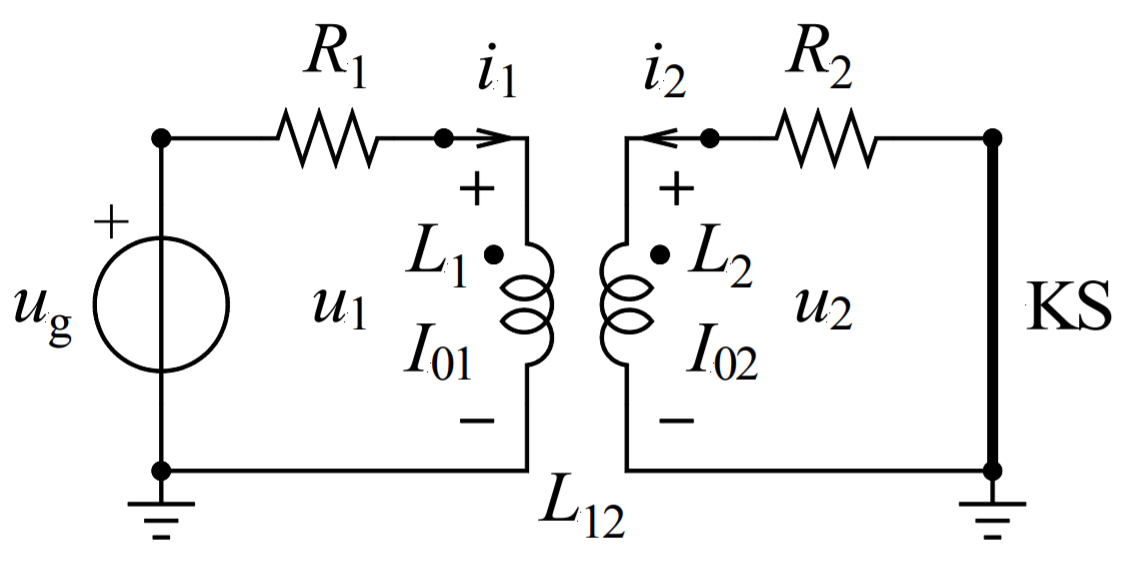
\includegraphics[scale = 0.55]{Figure10.png}\\
       Figure 10: Inductive Transformer.
   \end{center} 
    

    \textbf{Step 9.1.} Repeat steps 1.2-1.7.

    \begin{tcolorbox}[breakable, size=fbox, boxrule=1pt, pad at break*=1mm,colback=cellbackground, colframe=cellborder]
\prompt{In}{incolor}{62}{\boxspacing}
\begin{Verbatim}[commandchars=\\\{\}]
\PY{k+kn}{from} \PY{n+nn}{symPyCAP} \PY{k+kn}{import} \PY{n}{Circuit}
\PY{k+kn}{import} \PY{n+nn}{sympy}
\end{Verbatim}
\end{tcolorbox}

    \begin{tcolorbox}[breakable, size=fbox, boxrule=1pt, pad at break*=1mm,colback=cellbackground, colframe=cellborder]
\prompt{In}{incolor}{63}{\boxspacing}
\begin{Verbatim}[commandchars=\\\{\}]
\PY{n}{R} \PY{o}{=} \PY{n}{sympy}\PY{o}{.}\PY{n}{Symbol}\PY{p}{(}\PY{l+s+s1}{\PYZsq{}}\PY{l+s+s1}{R}\PY{l+s+s1}{\PYZsq{}}\PY{p}{,} \PY{n}{positive}\PY{o}{=}\PY{k+kc}{True}\PY{p}{)}
\PY{n}{L} \PY{o}{=} \PY{n}{sympy}\PY{o}{.}\PY{n}{Symbol}\PY{p}{(}\PY{l+s+s1}{\PYZsq{}}\PY{l+s+s1}{L}\PY{l+s+s1}{\PYZsq{}}\PY{p}{,} \PY{n}{positive}\PY{o}{=}\PY{k+kc}{True}\PY{p}{)}
\PY{n}{t} \PY{o}{=} \PY{n}{sympy}\PY{o}{.}\PY{n}{Symbol}\PY{p}{(}\PY{l+s+s1}{\PYZsq{}}\PY{l+s+s1}{t}\PY{l+s+s1}{\PYZsq{}}\PY{p}{)}
\end{Verbatim}
\end{tcolorbox}

    \begin{tcolorbox}[breakable, size=fbox, boxrule=1pt, pad at break*=1mm,colback=cellbackground, colframe=cellborder]
\prompt{In}{incolor}{64}{\boxspacing}
\begin{Verbatim}[commandchars=\\\{\}]
\PY{n}{Inductive\PYZus{}schematic} \PY{o}{=} \PY{p}{[}
    \PY{p}{[}\PY{l+s+s2}{\PYZdq{}}\PY{l+s+s2}{R}\PY{l+s+s2}{\PYZdq{}}\PY{p}{,} \PY{l+s+s2}{\PYZdq{}}\PY{l+s+s2}{R1}\PY{l+s+s2}{\PYZdq{}}\PY{p}{,} \PY{l+m+mi}{3}\PY{p}{,} \PY{l+m+mi}{1}\PY{p}{]}\PY{p}{,}
    \PY{p}{[}\PY{l+s+s2}{\PYZdq{}}\PY{l+s+s2}{R}\PY{l+s+s2}{\PYZdq{}}\PY{p}{,} \PY{l+s+s2}{\PYZdq{}}\PY{l+s+s2}{R2}\PY{l+s+s2}{\PYZdq{}}\PY{p}{,} \PY{l+m+mi}{0}\PY{p}{,} \PY{l+m+mi}{2}\PY{p}{]}\PY{p}{,}
    \PY{p}{[}\PY{l+s+s2}{\PYZdq{}}\PY{l+s+s2}{V}\PY{l+s+s2}{\PYZdq{}}\PY{p}{,} \PY{l+s+s2}{\PYZdq{}}\PY{l+s+s2}{Ug}\PY{l+s+s2}{\PYZdq{}}\PY{p}{,} \PY{l+m+mi}{3}\PY{p}{,} \PY{l+m+mi}{0}\PY{p}{]}\PY{p}{,}
    \PY{p}{[}\PY{l+s+s2}{\PYZdq{}}\PY{l+s+s2}{InductiveT}\PY{l+s+s2}{\PYZdq{}}\PY{p}{,} \PY{l+s+s2}{\PYZdq{}}\PY{l+s+s2}{InductiveT1}\PY{l+s+s2}{\PYZdq{}}\PY{p}{,} \PY{p}{[}\PY{l+m+mi}{1}\PY{p}{,}\PY{l+m+mi}{0}\PY{p}{]}\PY{p}{,} \PY{p}{[}\PY{l+m+mi}{2}\PY{p}{,}\PY{l+m+mi}{0}\PY{p}{]}\PY{p}{,} \PY{p}{[}\PY{l+s+s2}{\PYZdq{}}\PY{l+s+s2}{LT1\PYZus{}1}\PY{l+s+s2}{\PYZdq{}}\PY{p}{,}\PY{l+s+s2}{\PYZdq{}}\PY{l+s+s2}{LT1\PYZus{}2}\PY{l+s+s2}{\PYZdq{}}\PY{p}{,}\PY{l+s+s2}{\PYZdq{}}\PY{l+s+s2}{LT1\PYZus{}12}\PY{l+s+s2}{\PYZdq{}}\PY{p}{]}\PY{p}{,} \PY{p}{[}\PY{l+s+s2}{\PYZdq{}}\PY{l+s+s2}{Io1}\PY{l+s+s2}{\PYZdq{}}\PY{p}{,}\PY{l+s+s2}{\PYZdq{}}\PY{l+s+s2}{Io2}\PY{l+s+s2}{\PYZdq{}}\PY{p}{]}\PY{p}{]}
\PY{p}{]}
\end{Verbatim}
\end{tcolorbox}

    \begin{tcolorbox}[breakable, size=fbox, boxrule=1pt, pad at break*=1mm,colback=cellbackground, colframe=cellborder]
\prompt{In}{incolor}{65}{\boxspacing}
\begin{Verbatim}[commandchars=\\\{\}]
\PY{n}{Inductive_circuit} \PY{o}{=} \PY{n}{Circuit}\PY{p}{(}\PY{n}{Inductive\PYZus{}schematic}\PY{p}{)}
\end{Verbatim}
\end{tcolorbox}

    \begin{tcolorbox}[breakable, size=fbox, boxrule=1pt, pad at break*=1mm,colback=cellbackground, colframe=cellborder]
\prompt{In}{incolor}{66}{\boxspacing}
\begin{Verbatim}[commandchars=\\\{\}]
\PY{n}{Inductive_circuit}\PY{o}{.}\PY{n}{symPyCAP}\PY{p}{(}\PY{n}{replacement} \PY{o}{=} \PY{p}{\PYZob{}}\PY{l+s+s2}{\PYZdq{}}\PY{l+s+s2}{R1}\PY{l+s+s2}{\PYZdq{}} \PY{p}{:} \PY{n}{R}\PY{p}{,} \PY{l+s+s2}{\PYZdq{}}\PY{l+s+s2}{R2}\PY{l+s+s2}{\PYZdq{}} \PY{p}{:} \PY{n}{R}\PY{p}{,} \PY{l+s+s2}{\PYZdq{}}\PY{l+s+s2}{LT1\PYZus{}1}\PY{l+s+s2}{\PYZdq{}} \PY{p}{:} \PY{n}{L}\PY{p}{,} \PY{l+s+s2}{\PYZdq{}}\PY{l+s+s2}{LT1\PYZus{}2}\PY{l+s+s2}{\PYZdq{}} \PY{p}{:} \PY{n}{L}\PY{p}{,} \PY{l+s+s2}{\PYZdq{}}\PY{l+s+s2}{LT1\PYZus{}12}\PY{l+s+s2}{\PYZdq{}} \PY{p}{:} \PY{n}{L}\PY{o}{/}\PY{l+m+mi}{2}\PY{p}{\PYZcb{}}\PY{p}{)} 
\end{Verbatim}
\end{tcolorbox}

    \begin{tcolorbox}[breakable, size=fbox, boxrule=1pt, pad at break*=1mm,colback=cellbackground, colframe=cellborder]
\prompt{In}{incolor}{67}{\boxspacing}
\begin{Verbatim}[commandchars=\\\{\}]
\PY{n}{Inductive_circuit}\PY{o}{.}\PY{n}{print\PYZus{}specific\PYZus{}solutions}\PY{p}{(}\PY{p}{)}
\end{Verbatim}
\end{tcolorbox}

    \begin{Verbatim}[commandchars=\\\{\}]
V1 : L*(-3*Io1*L*R*s - 4*Io1*R**2 - 2*Io2*R**2 + 3*L*Ug*s**2 +
4*R*Ug*s)/(3*L**2*s**2 + 8*L*R*s + 4*R**2)

V2 : -L*R*(2*Io1*R + 3*Io2*L*s + 4*Io2*R - 2*Ug*s)/(3*L**2*s**2 + 8*L*R*s +
4*R**2)

V3 : Ug

IUg : -(3*Io1*L**2*s + 4*Io1*L*R + 2*Io2*L*R + 4*L*Ug*s + 4*R*Ug)/(3*L**2*s**2 +
8*L*R*s + 4*R**2)

IInductiveT1\_1 : (3*Io1*L**2*s + 4*Io1*L*R + 2*Io2*L*R + 4*L*Ug*s +
4*R*Ug)/(3*L**2*s**2 + 8*L*R*s + 4*R**2)

IInductiveT1\_2 : L*(2*Io1*R + 3*Io2*L*s + 4*Io2*R - 2*Ug*s)/(3*L**2*s**2 +
8*L*R*s + 4*R**2)

    \end{Verbatim}

    \textbf{Step 9.2.} The time-domain for \textbf{\textit{$i_1$}} and \textbf{\textit{$i_2$}}, for t
\textgreater{} 0, can be computed by SymPy's Inverse Laplace Transform
method. Excitation is assumed to be the Dirac delta-function of
strength Ug.

    \begin{tcolorbox}[breakable, size=fbox, boxrule=1pt, pad at break*=1mm,colback=cellbackground, colframe=cellborder]
\prompt{In}{incolor}{68}{\boxspacing}
\begin{Verbatim}[commandchars=\\\{\}]
\PY{n}{inverse\PYZus{}laplace\PYZus{}transform}\PY{p}{(}\PY{n}{Inductive_circuit}\PY{o}{.}\PY{n}{get\PYZus{}specific\PYZus{}solutions}\PY{p}{(}\PY{p}{)}\PY{p}{[}\PY{l+s+s2}{\PYZdq{}}\PY{l+s+s2}{IInductiveT1\PYZus{}2}\PY{l+s+s2}{\PYZdq{}}\PY{p}{]}\PY{p}{,}\PY{n}{s}\PY{p}{,}\PY{n}{t}\PY{p}{)}
\end{Verbatim}
\end{tcolorbox}
 
            
\prompt{Out}{outcolor}{68}{}
    
    $\displaystyle - \frac{Io_{1} e^{- \frac{2 R t}{L}} \theta\left(t\right)}{2} + \frac{Io_{1} e^{- \frac{2 R t}{3 L}} \theta\left(t\right)}{2} + \frac{Io_{2} e^{- \frac{2 R t}{L}} \theta\left(t\right)}{2} + \frac{Io_{2} e^{- \frac{2 R t}{3 L}} \theta\left(t\right)}{2} - \frac{Ug e^{- \frac{2 R t}{L}} \theta\left(t\right)}{L} + \frac{Ug e^{- \frac{2 R t}{3 L}} \theta\left(t\right)}{3 L}$

    

    \begin{tcolorbox}[breakable, size=fbox, boxrule=1pt, pad at break*=1mm,colback=cellbackground, colframe=cellborder]
\prompt{In}{incolor}{69}{\boxspacing}
\begin{Verbatim}[commandchars=\\\{\}]
\PY{n}{inverse\PYZus{}laplace\PYZus{}transform}\PY{p}{(}\PY{n}{Inductive_circuit}\PY{o}{.}\PY{n}{get\PYZus{}specific\PYZus{}solutions}\PY{p}{(}\PY{p}{)}\PY{p}{[}\PY{l+s+s2}{\PYZdq{}}\PY{l+s+s2}{IInductiveT1\PYZus{}1}\PY{l+s+s2}{\PYZdq{}}\PY{p}{]}\PY{p}{,}\PY{n}{s}\PY{p}{,}\PY{n}{t}\PY{p}{)}
\end{Verbatim}
\end{tcolorbox}
 
            
\prompt{Out}{outcolor}{69}{}
    
    $\displaystyle \frac{Io_{1} e^{- \frac{2 R t}{L}} \theta\left(t\right)}{2} + \frac{Io_{1} e^{- \frac{2 R t}{3 L}} \theta\left(t\right)}{2} - \frac{Io_{2} e^{- \frac{2 R t}{L}} \theta\left(t\right)}{2} + \frac{Io_{2} e^{- \frac{2 R t}{3 L}} \theta\left(t\right)}{2} + \frac{Ug e^{- \frac{2 R t}{L}} \theta\left(t\right)}{L} + \frac{Ug e^{- \frac{2 R t}{3 L}} \theta\left(t\right)}{3 L}$


    \begin{tcolorbox}[breakable, size=fbox, boxrule=1pt, pad at break*=1mm,colback=cellbackground, colframe=cellborder]
\prompt{In}{incolor}{70}{\boxspacing}
\begin{Verbatim}[commandchars=\\\{\}]
\PY{n}{ugt} \PY{o}{=} \PY{n}{Phi}\PY{o}{*}\PY{n}{DiracDelta}\PY{p}{(}\PY{n}{t}\PY{p}{)}
\end{Verbatim}
\end{tcolorbox}

    \begin{tcolorbox}[breakable, size=fbox, boxrule=1pt, pad at break*=1mm,colback=cellbackground, colframe=cellborder]
\prompt{In}{incolor}{71}{\boxspacing}
\begin{Verbatim}[commandchars=\\\{\}]
\PY{n}{ugs} \PY{o}{=} \PY{n}{laplace\PYZus{}transform}\PY{p}{(}\PY{n}{ugt}\PY{p}{,} \PY{n}{t}\PY{p}{,} \PY{n}{s}\PY{p}{)}
\end{Verbatim}
\end{tcolorbox}

    \begin{tcolorbox}[breakable, size=fbox, boxrule=1pt, pad at break*=1mm,colback=cellbackground, colframe=cellborder]
\prompt{In}{incolor}{72}{\boxspacing}
\begin{Verbatim}[commandchars=\\\{\}]
\PY{n}{ugs}
\end{Verbatim}
\end{tcolorbox}

            \begin{tcolorbox}[breakable, size=fbox, boxrule=.5pt, pad at break*=1mm, opacityfill=0]
\prompt{Out}{outcolor}{72}{\boxspacing}
\begin{Verbatim}[commandchars=\\\{\}]
(Phi*(1 - Heaviside(0)), -oo, True)
\end{Verbatim}
\end{tcolorbox}
        
    \begin{tcolorbox}[breakable, size=fbox, boxrule=1pt, pad at break*=1mm,colback=cellbackground, colframe=cellborder]
\prompt{In}{incolor}{73}{\boxspacing}
\begin{Verbatim}[commandchars=\\\{\}]
\PY{n}{Inductive\PYZus{}circuit}\PY{o}{.}\PY{n}{get\PYZus{}specific\PYZus{}solutions}\PY{p}{(}\PY{p}{)}\PY{p}{[}\PY{l+s+s2}{\PYZdq{}}\PY{l+s+s2}{IInductiveT1\PYZus{}2}\PY{l+s+s2}{\PYZdq{}}\PY{p}{]}\PY{o}{.}\PY{n}{subs}\PY{p}{(}\PY{n}{R}\PY{p}{,} \PY{n}{L}\PY{p}{)}
\end{Verbatim}
\end{tcolorbox}
 
            
\prompt{Out}{outcolor}{73}{}
    
    $\displaystyle \frac{\frac{Io_{1} L^{2}}{2} + \frac{3 Io_{2} L^{2} s}{4} + Io_{2} L^{2} - \frac{L Ug s}{2}}{\frac{3 L^{2} s^{2}}{4} + 2 L^{2} s + L^{2}}$

    

     

    \begin{center}\rule{0.5\linewidth}{0.5pt}\end{center}

    \hypertarget{example-10-lc-circuit}{%
\section*{\texorpdfstring{Example 10: LC circuit
}{Example 10: LC circuit }}\label{example10}}

An LC circuit is shown in Figure 11. Its resonant frequency is
\textbf{\textit{$w = \displaystyle \frac{1}{\sqrt{LC}}$}}. At this frequency, the
circuit response diverges.

    \begin{center}
   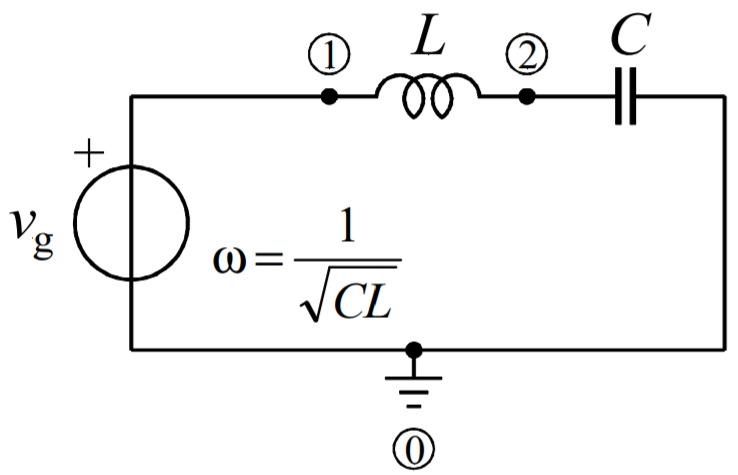
\includegraphics[scale = 0.45]{Figure11.PNG}\\
       Figure 11: LC circuit.
   \end{center} 
    

    \textbf{Step 10.1.} Repeat steps 1.2-1.7.

    \begin{tcolorbox}[breakable, size=fbox, boxrule=1pt, pad at break*=1mm,colback=cellbackground, colframe=cellborder]
\prompt{In}{incolor}{70}{\boxspacing}
\begin{Verbatim}[commandchars=\\\{\}]
\PY{k+kn}{from} \PY{n+nn}{symPyCAP} \PY{k+kn}{import} \PY{n}{Circuit}
\PY{k+kn}{import} \PY{n+nn}{sympy}
\end{Verbatim}
\end{tcolorbox}

    \begin{tcolorbox}[breakable, size=fbox, boxrule=1pt, pad at break*=1mm,colback=cellbackground, colframe=cellborder]
\prompt{In}{incolor}{71}{\boxspacing}
\begin{Verbatim}[commandchars=\\\{\}]
\PY{n}{C} \PY{o}{=} \PY{n}{sympy}\PY{o}{.}\PY{n}{Symbol}\PY{p}{(}\PY{l+s+s1}{\PYZsq{}}\PY{l+s+s1}{C}\PY{l+s+s1}{\PYZsq{}}\PY{p}{)}
\PY{n}{L} \PY{o}{=} \PY{n}{sympy}\PY{o}{.}\PY{n}{Symbol}\PY{p}{(}\PY{l+s+s1}{\PYZsq{}}\PY{l+s+s1}{L}\PY{l+s+s1}{\PYZsq{}}\PY{p}{)}
\end{Verbatim}
\end{tcolorbox}

    \begin{tcolorbox}[breakable, size=fbox, boxrule=1pt, pad at break*=1mm,colback=cellbackground, colframe=cellborder]
\prompt{In}{incolor}{72}{\boxspacing}
\begin{Verbatim}[commandchars=\\\{\}]
\PY{n}{LC\PYZus{}schematic} \PY{o}{=} \PY{p}{[}
    \PY{p}{[}\PY{l+s+s2}{\PYZdq{}}\PY{l+s+s2}{L}\PY{l+s+s2}{\PYZdq{}}\PY{p}{,} \PY{l+s+s2}{\PYZdq{}}\PY{l+s+s2}{L1}\PY{l+s+s2}{\PYZdq{}}\PY{p}{,} \PY{l+m+mi}{2}\PY{p}{,} \PY{l+m+mi}{1}\PY{p}{]}\PY{p}{,}
    \PY{p}{[}\PY{l+s+s2}{\PYZdq{}}\PY{l+s+s2}{C}\PY{l+s+s2}{\PYZdq{}}\PY{p}{,} \PY{l+s+s2}{\PYZdq{}}\PY{l+s+s2}{C1}\PY{l+s+s2}{\PYZdq{}}\PY{p}{,} \PY{l+m+mi}{0}\PY{p}{,} \PY{l+m+mi}{2}\PY{p}{]}\PY{p}{,}
    \PY{p}{[}\PY{l+s+s2}{\PYZdq{}}\PY{l+s+s2}{V}\PY{l+s+s2}{\PYZdq{}}\PY{p}{,} \PY{l+s+s2}{\PYZdq{}}\PY{l+s+s2}{Vg}\PY{l+s+s2}{\PYZdq{}}\PY{p}{,} \PY{l+m+mi}{1}\PY{p}{,} \PY{l+m+mi}{0}\PY{p}{]}\PY{p}{,}
\PY{p}{]}
\end{Verbatim}
\end{tcolorbox}

    \begin{tcolorbox}[breakable, size=fbox, boxrule=1pt, pad at break*=1mm,colback=cellbackground, colframe=cellborder]
\prompt{In}{incolor}{73}{\boxspacing}
\begin{Verbatim}[commandchars=\\\{\}]
\PY{n}{LC_circuit} \PY{o}{=} \PY{n}{Circuit}\PY{p}{(}\PY{n}{LC\PYZus{}schematic}\PY{p}{)}
\end{Verbatim}
\end{tcolorbox}

    \begin{tcolorbox}[breakable, size=fbox, boxrule=1pt, pad at break*=1mm,colback=cellbackground, colframe=cellborder]
\prompt{In}{incolor}{74}{\boxspacing}
\begin{Verbatim}[commandchars=\\\{\}]
\PY{n}{LC_circuit}\PY{o}{.}\PY{n}{symPyCAP}\PY{p}{(}\PY{n}{w} \PY{o}{=} \PY{l+m+mi}{1}\PY{o}{/}\PY{p}{(}\PY{n}{sympy}\PY{o}{.}\PY{n}{sqrt}\PY{p}{(}\PY{n}{L}\PY{o}{*}\PY{n}{C}\PY{p}{)}\PY{p}{)}\PY{p}{,} \PY{n}{replacement} \PY{o}{=} \PY{p}{\PYZob{}}\PY{l+s+s2}{\PYZdq{}}\PY{l+s+s2}{L1}\PY{l+s+s2}{\PYZdq{}} \PY{p}{:} \PY{n}{L}\PY{p}{,} \PY{l+s+s2}{\PYZdq{}}\PY{l+s+s2}{C1}\PY{l+s+s2}{\PYZdq{}} \PY{p}{:} \PY{n}{C}\PY{p}{\PYZcb{}}\PY{p}{)} 
\end{Verbatim}
\end{tcolorbox}

    \begin{tcolorbox}[breakable, size=fbox, boxrule=1pt, pad at break*=1mm,colback=cellbackground, colframe=cellborder]
\prompt{In}{incolor}{75}{\boxspacing}
\begin{Verbatim}[commandchars=\\\{\}]
\PY{n}{LC_circuit}\PY{o}{.}\PY{n}{print\PYZus{}specific\PYZus{}solutions}\PY{p}{(}\PY{p}{)}
\end{Verbatim}
\end{tcolorbox}

    \begin{Verbatim}[commandchars=\\\{\}]
Steady-state response does not exist at frequency 1/sqrt(C*L)
    \end{Verbatim}

    \begin{center}\rule{0.5\linewidth}{0.5pt}\end{center}

    \hypertarget{example-11-parallel-connection-of-voltage-generators}{%
\section*{\texorpdfstring{Example 11: Parallel connection of voltage
generators
}{Example 11: Parallel connection of voltage generators }}\label{example11}}

An untypical example is two voltage generators of different voltage
values. This circuit does not have a solution.

    \begin{center}
   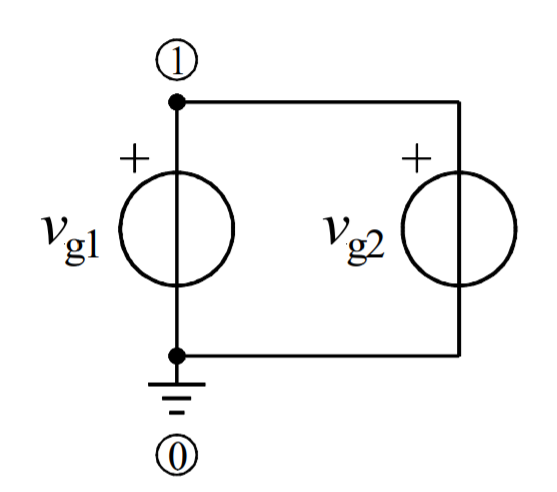
\includegraphics[scale = 0.4]{Figure12.PNG}\\
       Figure 12: Parallel connection of voltage generators.
   \end{center} 
    

    \textbf{Step 11.1.} Repeat necessary steps 1.2-1.7.

    \begin{tcolorbox}[breakable, size=fbox, boxrule=1pt, pad at break*=1mm,colback=cellbackground, colframe=cellborder]
\prompt{In}{incolor}{76}{\boxspacing}
\begin{Verbatim}[commandchars=\\\{\}]
\PY{k+kn}{from} \PY{n+nn}{symPyCAP} \PY{k+kn}{import} \PY{n}{Circuit}
\end{Verbatim}
\end{tcolorbox}

    \begin{tcolorbox}[breakable, size=fbox, boxrule=1pt, pad at break*=1mm,colback=cellbackground, colframe=cellborder]
\prompt{In}{incolor}{77}{\boxspacing}
\begin{Verbatim}[commandchars=\\\{\}]
\PY{n}{EE\PYZus{}schematic} \PY{o}{=} \PY{p}{[}
    \PY{p}{[}\PY{l+s+s2}{\PYZdq{}}\PY{l+s+s2}{V}\PY{l+s+s2}{\PYZdq{}}\PY{p}{,} \PY{l+s+s2}{\PYZdq{}}\PY{l+s+s2}{Vg1}\PY{l+s+s2}{\PYZdq{}}\PY{p}{,} \PY{l+m+mi}{0}\PY{p}{,} \PY{l+m+mi}{1}\PY{p}{]}\PY{p}{,}
    \PY{p}{[}\PY{l+s+s2}{\PYZdq{}}\PY{l+s+s2}{V}\PY{l+s+s2}{\PYZdq{}}\PY{p}{,} \PY{l+s+s2}{\PYZdq{}}\PY{l+s+s2}{Vg2}\PY{l+s+s2}{\PYZdq{}}\PY{p}{,} \PY{l+m+mi}{0}\PY{p}{,} \PY{l+m+mi}{1}\PY{p}{]}\PY{p}{,}
\PY{p}{]}
\end{Verbatim}
\end{tcolorbox}

    \begin{tcolorbox}[breakable, size=fbox, boxrule=1pt, pad at break*=1mm,colback=cellbackground, colframe=cellborder]
\prompt{In}{incolor}{78}{\boxspacing}
\begin{Verbatim}[commandchars=\\\{\}]
\PY{n}{EE_circuit} \PY{o}{=} \PY{n}{Circuit}\PY{p}{(}\PY{n}{EE\PYZus{}schematic}\PY{p}{)}
\end{Verbatim}
\end{tcolorbox}

    \begin{tcolorbox}[breakable, size=fbox, boxrule=1pt, pad at break*=1mm,colback=cellbackground, colframe=cellborder]
\prompt{In}{incolor}{79}{\boxspacing}
\begin{Verbatim}[commandchars=\\\{\}]
\PY{n}{EE_circuit}\PY{o}{.}\PY{n}{symPyCAP}\PY{p}{(}\PY{p}{)}
\end{Verbatim}
\end{tcolorbox}

    \begin{tcolorbox}[breakable, size=fbox, boxrule=1pt, pad at break*=1mm,colback=cellbackground, colframe=cellborder]
\prompt{In}{incolor}{80}{\boxspacing}
\begin{Verbatim}[commandchars=\\\{\}]
\PY{n}{EE_circuit}\PY{o}{.}\PY{n}{print\PYZus{}solutions}\PY{p}{(}\PY{p}{)}
\end{Verbatim}
\end{tcolorbox}

    \begin{Verbatim}[commandchars=\\\{\}]
Solution does not exist!
    \end{Verbatim}
    The circuit is not well-behaved because the element equations, KCL and KVL cannot hold simultaneously.

    \begin{center}\rule{0.5\linewidth}{0.5pt}\end{center}

    \hypertarget{example-12-ideal-transformers}{%
\section*{\texorpdfstring{Example 12: Ideal transformers
}{Example 12: Ideal transformers }}\label{example12}}

Two ideal transformers, which are cascaded to get the
higher gain, are shown in Figure 13.

    \begin{center}    
    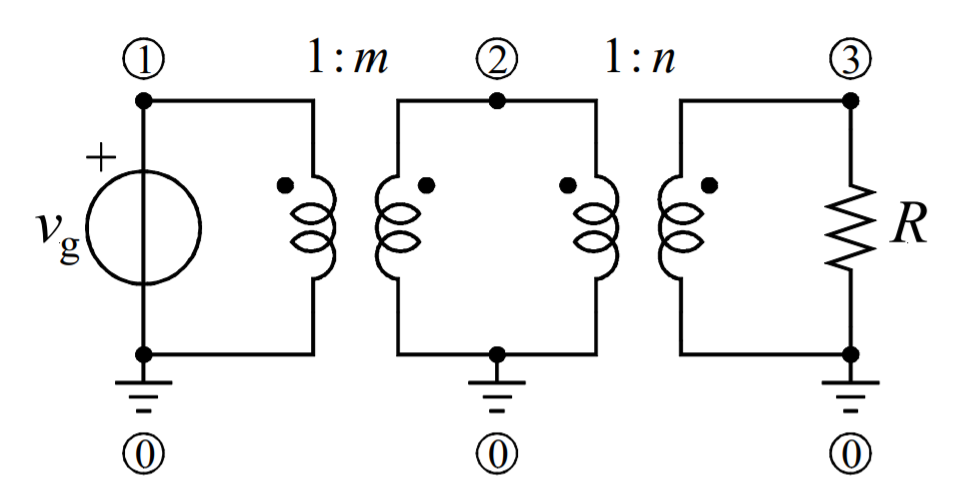
\includegraphics[scale = 0.55]{Figure13.PNG}\\
    Figure 13: Ideal transformers.
    \end{center}
    

    \textbf{Step 12.1.} Repeat necessary steps 1.2-1.7.

    \begin{tcolorbox}[breakable, size=fbox, boxrule=1pt, pad at break*=1mm,colback=cellbackground, colframe=cellborder]
\prompt{In}{incolor}{81}{\boxspacing}
\begin{Verbatim}[commandchars=\\\{\}]
\PY{k+kn}{from} \PY{n+nn}{symPyCAP} \PY{k+kn}{import} \PY{n}{Circuit}
\PY{k+kn}{import} \PY{n+nn}{sympy}
\end{Verbatim}
\end{tcolorbox}

    \begin{tcolorbox}[breakable, size=fbox, boxrule=1pt, pad at break*=1mm,colback=cellbackground, colframe=cellborder]
\prompt{In}{incolor}{82}{\boxspacing}
\begin{Verbatim}[commandchars=\\\{\}]
\PY{n}{m} \PY{o}{=} \PY{n}{sympy}\PY{o}{.}\PY{n}{Symbol}\PY{p}{(}\PY{l+s+s1}{\PYZsq{}}\PY{l+s+s1}{m}\PY{l+s+s1}{\PYZsq{}}\PY{p}{)}
\PY{n}{n} \PY{o}{=} \PY{n}{sympy}\PY{o}{.}\PY{n}{Symbol}\PY{p}{(}\PY{l+s+s1}{\PYZsq{}}\PY{l+s+s1}{n}\PY{l+s+s1}{\PYZsq{}}\PY{p}{)}
\end{Verbatim}
\end{tcolorbox}

    \begin{tcolorbox}[breakable, size=fbox, boxrule=1pt, pad at break*=1mm,colback=cellbackground, colframe=cellborder]
\prompt{In}{incolor}{83}{\boxspacing}
\begin{Verbatim}[commandchars=\\\{\}]
\PY{n}{Ideal\PYZus{}schematic} \PY{o}{=} \PY{p}{[}
    \PY{p}{[}\PY{l+s+s2}{\PYZdq{}}\PY{l+s+s2}{V}\PY{l+s+s2}{\PYZdq{}}\PY{p}{,} \PY{l+s+s2}{\PYZdq{}}\PY{l+s+s2}{Vg}\PY{l+s+s2}{\PYZdq{}}\PY{p}{,} \PY{l+m+mi}{1}\PY{p}{,} \PY{l+m+mi}{0}\PY{p}{]}\PY{p}{,}
    \PY{p}{[}\PY{l+s+s2}{\PYZdq{}}\PY{l+s+s2}{R}\PY{l+s+s2}{\PYZdq{}}\PY{p}{,} \PY{l+s+s2}{\PYZdq{}}\PY{l+s+s2}{R1}\PY{l+s+s2}{\PYZdq{}}\PY{p}{,} \PY{l+m+mi}{3}\PY{p}{,} \PY{l+m+mi}{0}\PY{p}{]}\PY{p}{,}
    \PY{p}{[}\PY{l+s+s2}{\PYZdq{}}\PY{l+s+s2}{IdealT}\PY{l+s+s2}{\PYZdq{}}\PY{p}{,} \PY{l+s+s2}{\PYZdq{}}\PY{l+s+s2}{IT1}\PY{l+s+s2}{\PYZdq{}}\PY{p}{,} \PY{p}{[}\PY{l+m+mi}{2}\PY{p}{,}\PY{l+m+mi}{0}\PY{p}{]}\PY{p}{,} \PY{p}{[}\PY{l+m+mi}{1}\PY{p}{,}\PY{l+m+mi}{0}\PY{p}{]}\PY{p}{,} \PY{l+s+s2}{\PYZdq{}}\PY{l+s+s2}{m}\PY{l+s+s2}{\PYZdq{}}\PY{p}{]}\PY{p}{,}
    \PY{p}{[}\PY{l+s+s2}{\PYZdq{}}\PY{l+s+s2}{IdealT}\PY{l+s+s2}{\PYZdq{}}\PY{p}{,} \PY{l+s+s2}{\PYZdq{}}\PY{l+s+s2}{IT2}\PY{l+s+s2}{\PYZdq{}}\PY{p}{,} \PY{p}{[}\PY{l+m+mi}{3}\PY{p}{,}\PY{l+m+mi}{0}\PY{p}{]}\PY{p}{,} \PY{p}{[}\PY{l+m+mi}{2}\PY{p}{,}\PY{l+m+mi}{0}\PY{p}{]}\PY{p}{,} \PY{l+s+s2}{\PYZdq{}}\PY{l+s+s2}{n}\PY{l+s+s2}{\PYZdq{}}\PY{p}{]}
\PY{p}{]}
\end{Verbatim}
\end{tcolorbox}

    \begin{tcolorbox}[breakable, size=fbox, boxrule=1pt, pad at break*=1mm,colback=cellbackground, colframe=cellborder]
\prompt{In}{incolor}{84}{\boxspacing}
\begin{Verbatim}[commandchars=\\\{\}]
\PY{n}{Ideal_circuit} \PY{o}{=} \PY{n}{Circuit}\PY{p}{(}\PY{n}{Ideal\PYZus{}schematic}\PY{p}{)}
\end{Verbatim}
\end{tcolorbox}

    \begin{tcolorbox}[breakable, size=fbox, boxrule=1pt, pad at break*=1mm,colback=cellbackground, colframe=cellborder]
\prompt{In}{incolor}{85}{\boxspacing}
\begin{Verbatim}[commandchars=\\\{\}]
\PY{n}{Ideal_circuit}\PY{o}{.}\PY{n}{symPyCAP}\PY{p}{(}\PY{p}{)}
\end{Verbatim}
\end{tcolorbox}

    \begin{tcolorbox}[breakable, size=fbox, boxrule=1pt, pad at break*=1mm,colback=cellbackground, colframe=cellborder]
\prompt{In}{incolor}{86}{\boxspacing}
\begin{Verbatim}[commandchars=\\\{\}]
\PY{n}{Ideal_circuit}\PY{o}{.}\PY{n}{print\PYZus{}solutions}\PY{p}{(}\PY{p}{)}
\end{Verbatim}
\end{tcolorbox}

    \begin{Verbatim}[commandchars=\\\{\}]
V1 : Vg

V2 : Vg*m

V3 : Vg*m*n

IE1 : -Vg*m**2*n**2/R1

IIT1 : -Vg*m*n**2/R1

IIT2 : -Vg*m*n/R1

    \end{Verbatim}

    \begin{center}\rule{0.5\linewidth}{0.5pt}\end{center}

    \hypertarget{example-13-voltage-divider}{%
\section*{Example 13: Voltage
divider}\label{example13}}

A voltage divider with two resistors and a voltage generator is shown in
Figure 14.

 \begin{center}    
    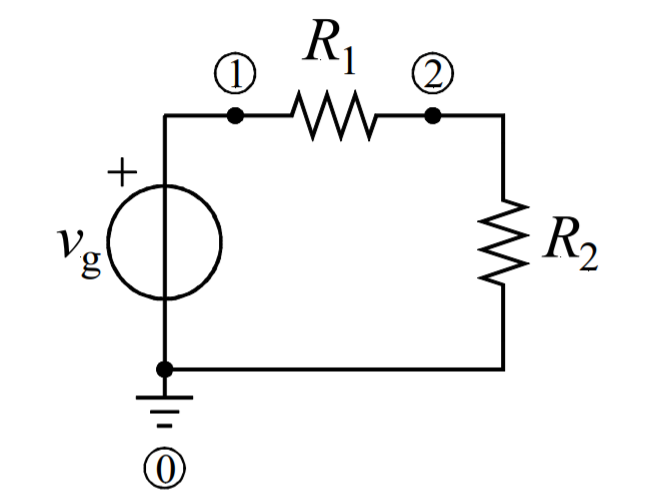
\includegraphics[scale = 0.4]{Figure14.PNG}\\
    Figure 14: Voltage divider.
    \end{center}
    

    \textbf{Step 13.1.} Repeat necessary steps 1.2-1.7.

    \begin{tcolorbox}[breakable, size=fbox, boxrule=1pt, pad at break*=1mm,colback=cellbackground, colframe=cellborder]
\prompt{In}{incolor}{91}{\boxspacing}
\begin{Verbatim}[commandchars=\\\{\}]
\PY{k+kn}{from} \PY{n+nn}{symPyCAP} \PY{k+kn}{import} \PY{n}{Circuit}
\PY{k+kn}{from} \PY{n+nn}{sympy} \PY{k+kn}{import} \PY{o}{*}
\end{Verbatim}
\end{tcolorbox}

    \begin{tcolorbox}[breakable, size=fbox, boxrule=1pt, pad at break*=1mm,colback=cellbackground, colframe=cellborder]
\prompt{In}{incolor}{92}{\boxspacing}
\begin{Verbatim}[commandchars=\\\{\}]
\PY{n}{Voltage\PYZus{}divider\PYZus{}schematic} \PY{o}{=} \PY{p}{[}
    \PY{p}{[}\PY{l+s+s2}{\PYZdq{}}\PY{l+s+s2}{V}\PY{l+s+s2}{\PYZdq{}}\PY{p}{,} \PY{l+s+s2}{\PYZdq{}}\PY{l+s+s2}{Vg}\PY{l+s+s2}{\PYZdq{}}\PY{p}{,} \PY{l+m+mi}{1}\PY{p}{,} \PY{l+m+mi}{0}\PY{p}{]}\PY{p}{,}
    \PY{p}{[}\PY{l+s+s2}{\PYZdq{}}\PY{l+s+s2}{R}\PY{l+s+s2}{\PYZdq{}}\PY{p}{,} \PY{l+s+s2}{\PYZdq{}}\PY{l+s+s2}{R1}\PY{l+s+s2}{\PYZdq{}}\PY{p}{,} \PY{l+m+mi}{1}\PY{p}{,} \PY{l+m+mi}{2}\PY{p}{]}\PY{p}{,}
    \PY{p}{[}\PY{l+s+s2}{\PYZdq{}}\PY{l+s+s2}{R}\PY{l+s+s2}{\PYZdq{}}\PY{p}{,} \PY{l+s+s2}{\PYZdq{}}\PY{l+s+s2}{R2}\PY{l+s+s2}{\PYZdq{}}\PY{p}{,} \PY{l+m+mi}{2}\PY{p}{,} \PY{l+m+mi}{0}\PY{p}{]}
\PY{p}{]}
\end{Verbatim}
\end{tcolorbox}

    \begin{tcolorbox}[breakable, size=fbox, boxrule=1pt, pad at break*=1mm,colback=cellbackground, colframe=cellborder]
\prompt{In}{incolor}{93}{\boxspacing}
\begin{Verbatim}[commandchars=\\\{\}]
\PY{n}{Voltage\PYZus{}divider\PYZus{}circuit} \PY{o}{=} \PY{n}{Circuit}\PY{p}{(}\PY{n}{Voltage\PYZus{}divider\PYZus{}schematic}\PY{p}{)}
\end{Verbatim}
\end{tcolorbox}

    \begin{tcolorbox}[breakable, size=fbox, boxrule=1pt, pad at break*=1mm,colback=cellbackground, colframe=cellborder]
\prompt{In}{incolor}{94}{\boxspacing}
\begin{Verbatim}[commandchars=\\\{\}]
\PY{n}{Voltage\PYZus{}divider\PYZus{}circuit}\PY{o}{.}\PY{n}{symPyCAP}\PY{p}{(}\PY{p}{)}
\end{Verbatim}
\end{tcolorbox}

    \begin{tcolorbox}[breakable, size=fbox, boxrule=1pt, pad at break*=1mm,colback=cellbackground, colframe=cellborder]
\prompt{In}{incolor}{95}{\boxspacing}
\begin{Verbatim}[commandchars=\\\{\}]
\PY{n}{Voltage\PYZus{}divider\PYZus{}circuit}\PY{o}{.}\PY{n}{print\PYZus{}solutions}\PY{p}{(}\PY{p}{)}
\end{Verbatim}
\end{tcolorbox}

    \begin{Verbatim}[commandchars=\\\{\}]
V1 : Vg

V2 : R2*Vg/(R1 + R2)

IVg : -Vg/(R1 + R2)

    \end{Verbatim}

    \textbf{Step 13.2.} Easily obtain the voltages across resistors R1 and
R2.

    \begin{tcolorbox}[breakable, size=fbox, boxrule=1pt, pad at break*=1mm,colback=cellbackground, colframe=cellborder]
\prompt{In}{incolor}{96}{\boxspacing}
\begin{Verbatim}[commandchars=\\\{\}]
\PY{n}{UR1} \PY{o}{=} \PY{n}{simplify}\PY{p}{(}\PY{n}{Voltage\PYZus{}divider\PYZus{}circuit}\PY{o}{.}\PY{n}{get\PYZus{}solutions}\PY{p}{(}\PY{p}{)}\PY{p}{[}\PY{l+s+s2}{\PYZdq{}}\PY{l+s+s2}{V1}\PY{l+s+s2}{\PYZdq{}}\PY{p}{]}\PY{o}{\PYZhy{}}\PY{n}{Voltage\PYZus{}divider\PYZus{}circuit}\PY{o}{.}\PY{n}{get\PYZus{}solutions}\PY{p}{(}\PY{p}{)}\PY{p}{[}\PY{l+s+s2}{\PYZdq{}}\PY{l+s+s2}{V2}\PY{l+s+s2}{\PYZdq{}}\PY{p}{]}\PY{p}{)}
\end{Verbatim}
\end{tcolorbox}

    \begin{tcolorbox}[breakable, size=fbox, boxrule=1pt, pad at break*=1mm,colback=cellbackground, colframe=cellborder]
\prompt{In}{incolor}{97}{\boxspacing}
\begin{Verbatim}[commandchars=\\\{\}]
\PY{n}{UR1}
\end{Verbatim}
\end{tcolorbox}
 
            
\prompt{Out}{outcolor}{97}{}
    
    $\displaystyle \frac{R_{1} Vg}{R_{1} + R_{2}}$

    

    \begin{tcolorbox}[breakable, size=fbox, boxrule=1pt, pad at break*=1mm,colback=cellbackground, colframe=cellborder]
\prompt{In}{incolor}{98}{\boxspacing}
\begin{Verbatim}[commandchars=\\\{\}]
\PY{n}{UR2} \PY{o}{=} \PY{n}{Voltage\PYZus{}divider\PYZus{}circuit}\PY{o}{.}\PY{n}{get\PYZus{}solutions}\PY{p}{(}\PY{p}{)}\PY{p}{[}\PY{l+s+s2}{\PYZdq{}}\PY{l+s+s2}{V2}\PY{l+s+s2}{\PYZdq{}}\PY{p}{]}
\end{Verbatim}
\end{tcolorbox}

    \begin{tcolorbox}[breakable, size=fbox, boxrule=1pt, pad at break*=1mm,colback=cellbackground, colframe=cellborder]
\prompt{In}{incolor}{99}{\boxspacing}
\begin{Verbatim}[commandchars=\\\{\}]
\PY{n}{UR2}
\end{Verbatim}
\end{tcolorbox}
 
            
\prompt{Out}{outcolor}{99}{}
    
    $\displaystyle \frac{R_{2} Vg}{R_{1} + R_{2}}$

    

    \begin{center}\rule{0.5\linewidth}{0.5pt}\end{center}

    \hypertarget{single-element-circuits}{%
\section*{Single element circuits}\label{single-element-circuits}}


The circuits analysed by SymPyCAP should have at least two nodes, ground
node and node 1.

    \hypertarget{example-14.1-voltage-generator---open-circuit}{%
\subsection*{\texorpdfstring{Example 14.1: Voltage generator - open
circuit
}{Example 14.1: Voltage generator - open circuit }}\label{example141}}

     \begin{center}    
    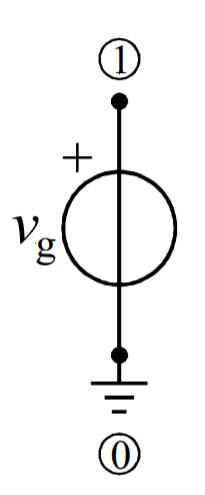
\includegraphics[scale = 0.4]{Figure15.PNG}\\
    Figure 15: Voltage generator - open circuit.
    \end{center}
    

    \textbf{Step 14.1.1.} Repeat necessary steps 1.2-1.7.

    \begin{tcolorbox}[breakable, size=fbox, boxrule=1pt, pad at break*=1mm,colback=cellbackground, colframe=cellborder]
\prompt{In}{incolor}{100}{\boxspacing}
\begin{Verbatim}[commandchars=\\\{\}]
\PY{k+kn}{from} \PY{n+nn}{symPyCAP} \PY{k+kn}{import} \PY{n}{Circuit}
\end{Verbatim}
\end{tcolorbox}

    \begin{tcolorbox}[breakable, size=fbox, boxrule=1pt, pad at break*=1mm,colback=cellbackground, colframe=cellborder]
\prompt{In}{incolor}{101}{\boxspacing}
\begin{Verbatim}[commandchars=\\\{\}]
\PY{n}{Generator\PYZus{}open\PYZus{}schematic} \PY{o}{=} \PY{p}{[}
    \PY{p}{[}\PY{l+s+s2}{\PYZdq{}}\PY{l+s+s2}{V}\PY{l+s+s2}{\PYZdq{}}\PY{p}{,} \PY{l+s+s2}{\PYZdq{}}\PY{l+s+s2}{Vg}\PY{l+s+s2}{\PYZdq{}}\PY{p}{,} \PY{l+m+mi}{1}\PY{p}{,} \PY{l+m+mi}{0}\PY{p}{]}
\PY{p}{]}
\end{Verbatim}
\end{tcolorbox}

    \begin{tcolorbox}[breakable, size=fbox, boxrule=1pt, pad at break*=1mm,colback=cellbackground, colframe=cellborder]
\prompt{In}{incolor}{102}{\boxspacing}
\begin{Verbatim}[commandchars=\\\{\}]
\PY{n}{Voltage\PYZus{}open\PYZus{}circuit} \PY{o}{=} \PY{n}{Circuit}\PY{p}{(}\PY{n}{Generator\PYZus{}open\PYZus{}schematic}\PY{p}{)}
\end{Verbatim}
\end{tcolorbox}

    \begin{tcolorbox}[breakable, size=fbox, boxrule=1pt, pad at break*=1mm,colback=cellbackground, colframe=cellborder]
\prompt{In}{incolor}{103}{\boxspacing}
\begin{Verbatim}[commandchars=\\\{\}]
\PY{n}{Voltage\PYZus{}open\PYZus{}circuit}\PY{o}{.}\PY{n}{symPyCAP}\PY{p}{(}\PY{p}{)}
\end{Verbatim}
\end{tcolorbox}

    \begin{tcolorbox}[breakable, size=fbox, boxrule=1pt, pad at break*=1mm,colback=cellbackground, colframe=cellborder]
\prompt{In}{incolor}{104}{\boxspacing}
\begin{Verbatim}[commandchars=\\\{\}]
\PY{n}{Voltage\PYZus{}open\PYZus{}circuit}\PY{o}{.}\PY{n}{print\PYZus{}solutions}\PY{p}{(}\PY{p}{)}
\end{Verbatim}
\end{tcolorbox}

    \begin{Verbatim}[commandchars=\\\{\}]
V1 : Vg

IVg : 0

    \end{Verbatim}

    \hypertarget{example-14.2-voltage-generator---closed-circuit}{%
\subsection*{\texorpdfstring{Example 14.2: Voltage generator - closed
circuit
}{Example 14.2: Voltage generator - closed circuit }}\label{example142}}

     \begin{center}    
    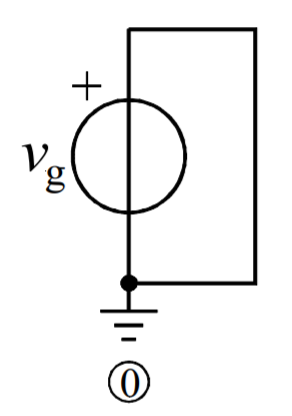
\includegraphics[scale = 0.4]{Figure16.PNG}\\
    Figure 16: Voltage generator - closed circuit.
    \end{center}
    

    \textbf{Step 14.2.1.} Repeat necessary steps 1.2-1.7.

    \begin{tcolorbox}[breakable, size=fbox, boxrule=1pt, pad at break*=1mm,colback=cellbackground, colframe=cellborder]
\prompt{In}{incolor}{105}{\boxspacing}
\begin{Verbatim}[commandchars=\\\{\}]
\PY{k+kn}{from} \PY{n+nn}{symPyCAP} \PY{k+kn}{import} \PY{n}{Circuit}
\end{Verbatim}
\end{tcolorbox}

    \begin{tcolorbox}[breakable, size=fbox, boxrule=1pt, pad at break*=1mm,colback=cellbackground, colframe=cellborder]
\prompt{In}{incolor}{106}{\boxspacing}
\begin{Verbatim}[commandchars=\\\{\}]
\PY{n}{Generator\PYZus{}closed\PYZus{}schematic} \PY{o}{=} \PY{p}{[}
    \PY{p}{[}\PY{l+s+s2}{\PYZdq{}}\PY{l+s+s2}{V}\PY{l+s+s2}{\PYZdq{}}\PY{p}{,} \PY{l+s+s2}{\PYZdq{}}\PY{l+s+s2}{Vg}\PY{l+s+s2}{\PYZdq{}}\PY{p}{,} \PY{l+m+mi}{0}\PY{p}{,} \PY{l+m+mi}{0}\PY{p}{]}
\PY{p}{]}
\end{Verbatim}
\end{tcolorbox}

    \begin{tcolorbox}[breakable, size=fbox, boxrule=1pt, pad at break*=1mm,colback=cellbackground, colframe=cellborder]
\prompt{In}{incolor}{107}{\boxspacing}
\begin{Verbatim}[commandchars=\\\{\}]
\PY{n}{Voltage\PYZus{}closed\PYZus{}circuit} \PY{o}{=} \PY{n}{Circuit}\PY{p}{(}\PY{n}{Generator\PYZus{}closed\PYZus{}schematic}\PY{p}{)}
\end{Verbatim}
\end{tcolorbox}

    \begin{tcolorbox}[breakable, size=fbox, boxrule=1pt, pad at break*=1mm,colback=cellbackground, colframe=cellborder]
\prompt{In}{incolor}{108}{\boxspacing}
\begin{Verbatim}[commandchars=\\\{\}]
\PY{n}{Voltage\PYZus{}closed\PYZus{}circuit}\PY{o}{.}\PY{n}{symPyCAP}\PY{p}{(}\PY{p}{)}
\end{Verbatim}
\end{tcolorbox}

    \begin{tcolorbox}[breakable, size=fbox, boxrule=1pt, pad at break*=1mm,colback=cellbackground, colframe=cellborder]
\prompt{In}{incolor}{109}{\boxspacing}
\begin{Verbatim}[commandchars=\\\{\}]
\PY{n}{Voltage\PYZus{}closed\PYZus{}circuit}\PY{o}{.}\PY{n}{print\PYZus{}solutions}\PY{p}{(}\PY{p}{)}
\end{Verbatim}
\end{tcolorbox}

    \begin{Verbatim}[commandchars=\\\{\}]
Solution does not exist!
    \end{Verbatim}

    \begin{center}\rule{0.5\linewidth}{0.5pt}\end{center}

    \hypertarget{example-15.1-current-generator---closed-circuit}{%
\subsection*{\texorpdfstring{Example 15.1: Current generator - closed
circuit
}{Example 15.1: Current generator - closed circuit }}\label{example151}}

     \begin{center}    
    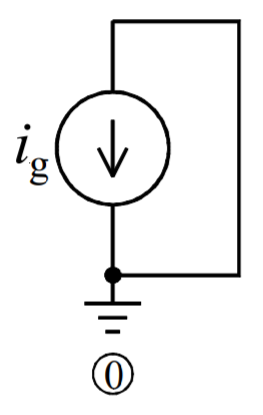
\includegraphics[scale = 0.4]{Figure17.PNG}\\
    Figure 17: Current generator - closed circuit.
    \end{center}

    \textbf{Step 15.1.1.} Repeat necessary steps 1.2-1.7.

    \begin{tcolorbox}[breakable, size=fbox, boxrule=1pt, pad at break*=1mm,colback=cellbackground, colframe=cellborder]
\prompt{In}{incolor}{110}{\boxspacing}
\begin{Verbatim}[commandchars=\\\{\}]
\PY{k+kn}{from} \PY{n+nn}{symPyCAP} \PY{k+kn}{import} \PY{n}{Circuit}
\end{Verbatim}
\end{tcolorbox}

    \begin{tcolorbox}[breakable, size=fbox, boxrule=1pt, pad at break*=1mm,colback=cellbackground, colframe=cellborder]
\prompt{In}{incolor}{111}{\boxspacing}
\begin{Verbatim}[commandchars=\\\{\}]
\PY{n}{Generator\PYZus{}closed\PYZus{}schematic} \PY{o}{=} \PY{p}{[}
    \PY{p}{[}\PY{l+s+s2}{\PYZdq{}}\PY{l+s+s2}{I}\PY{l+s+s2}{\PYZdq{}}\PY{p}{,} \PY{l+s+s2}{\PYZdq{}}\PY{l+s+s2}{Ig}\PY{l+s+s2}{\PYZdq{}}\PY{p}{,} \PY{l+m+mi}{0}\PY{p}{,} \PY{l+m+mi}{0}\PY{p}{]}
\PY{p}{]}
\end{Verbatim}
\end{tcolorbox}

    \begin{tcolorbox}[breakable, size=fbox, boxrule=1pt, pad at break*=1mm,colback=cellbackground, colframe=cellborder]
\prompt{In}{incolor}{112}{\boxspacing}
\begin{Verbatim}[commandchars=\\\{\}]
\PY{n}{Current\PYZus{}closed\PYZus{}circuit} \PY{o}{=} \PY{n}{Circuit}\PY{p}{(}\PY{n}{Generator\PYZus{}closed\PYZus{}schematic}\PY{p}{)}
\end{Verbatim}
\end{tcolorbox}

    \begin{tcolorbox}[breakable, size=fbox, boxrule=1pt, pad at break*=1mm,colback=cellbackground, colframe=cellborder]
\prompt{In}{incolor}{113}{\boxspacing}
\begin{Verbatim}[commandchars=\\\{\}]
\PY{n}{Current\PYZus{}closed\PYZus{}circuit}\PY{o}{.}\PY{n}{symPyCAP}\PY{p}{(}\PY{p}{)}
\end{Verbatim}
\end{tcolorbox}

    \begin{tcolorbox}[breakable, size=fbox, boxrule=1pt, pad at break*=1mm,colback=cellbackground, colframe=cellborder]
\prompt{In}{incolor}{114}{\boxspacing}
\begin{Verbatim}[commandchars=\\\{\}]
\PY{n}{Current\PYZus{}closed\PYZus{}circuit}\PY{o}{.}\PY{n}{print\PYZus{}solutions}\PY{p}{(}\PY{p}{)}
\end{Verbatim}
\end{tcolorbox}

    \begin{Verbatim}[commandchars=\\\{\}]
Solution does not exist!
    \end{Verbatim}

    \hypertarget{example-15.2-current-generator---open-circuit}{%
\subsection*{\texorpdfstring{Example 15.2: Current generator - open
circuit
}{Example 15.2: Current generator - open circuit }}\label{example152}}
    
    \begin{center}
    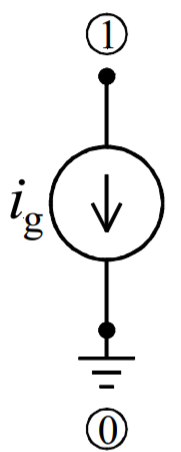
\includegraphics[scale = 0.4]{Figure18.PNG}\\
    Figure 18: Current generator - open circuit.
    \end{center}

    \textbf{Step 15.1.1.} Repeat necessary steps 1.2-1.7.

    \begin{tcolorbox}[breakable, size=fbox, boxrule=1pt, pad at break*=1mm,colback=cellbackground, colframe=cellborder]
\prompt{In}{incolor}{115}{\boxspacing}
\begin{Verbatim}[commandchars=\\\{\}]
\PY{k+kn}{from} \PY{n+nn}{symPyCAP} \PY{k+kn}{import} \PY{n}{Circuit}
\end{Verbatim}
\end{tcolorbox}

    \begin{tcolorbox}[breakable, size=fbox, boxrule=1pt, pad at break*=1mm,colback=cellbackground, colframe=cellborder]
\prompt{In}{incolor}{116}{\boxspacing}
\begin{Verbatim}[commandchars=\\\{\}]
\PY{n}{Generator\PYZus{}open\PYZus{}schematic} \PY{o}{=} \PY{p}{[}
    \PY{p}{[}\PY{l+s+s2}{\PYZdq{}}\PY{l+s+s2}{I}\PY{l+s+s2}{\PYZdq{}}\PY{p}{,} \PY{l+s+s2}{\PYZdq{}}\PY{l+s+s2}{Ig}\PY{l+s+s2}{\PYZdq{}}\PY{p}{,} \PY{l+m+mi}{1}\PY{p}{,} \PY{l+m+mi}{0}\PY{p}{]}
\PY{p}{]}
\end{Verbatim}
\end{tcolorbox}

    \begin{tcolorbox}[breakable, size=fbox, boxrule=1pt, pad at break*=1mm,colback=cellbackground, colframe=cellborder]
\prompt{In}{incolor}{117}{\boxspacing}
\begin{Verbatim}[commandchars=\\\{\}]
\PY{n}{Current\PYZus{}open\PYZus{}circuit} \PY{o}{=} \PY{n}{Circuit}\PY{p}{(}\PY{n}{Generator\PYZus{}open\PYZus{}schematic}\PY{p}{)}
\end{Verbatim}
\end{tcolorbox}

    \begin{tcolorbox}[breakable, size=fbox, boxrule=1pt, pad at break*=1mm,colback=cellbackground, colframe=cellborder]
\prompt{In}{incolor}{118}{\boxspacing}
\begin{Verbatim}[commandchars=\\\{\}]
\PY{n}{Current\PYZus{}open\PYZus{}circuit}\PY{o}{.}\PY{n}{symPyCAP}\PY{p}{(}\PY{p}{)}
\end{Verbatim}
\end{tcolorbox}

    \begin{tcolorbox}[breakable, size=fbox, boxrule=1pt, pad at break*=1mm,colback=cellbackground, colframe=cellborder]
\prompt{In}{incolor}{119}{\boxspacing}
\begin{Verbatim}[commandchars=\\\{\}]
\PY{n}{Current\PYZus{}open\PYZus{}circuit}\PY{o}{.}\PY{n}{print\PYZus{}solutions}\PY{p}{(}\PY{p}{)}
\end{Verbatim}
\end{tcolorbox}

    \begin{Verbatim}[commandchars=\\\{\}]
Solution does not exist!
    \end{Verbatim}

    \begin{center}\rule{0.5\linewidth}{0.5pt}\end{center}

    \hypertarget{example-16.1-capacitor-with-initial-state---open-circuit}{%
\subsection*{\texorpdfstring{Example 16.1: Capacitor with initial state -
open circuit
}{Example 16.1: Capacitor with initial state - open circuit }}\label{example161}}
   
    \begin{center}
    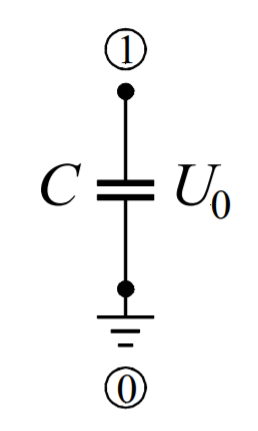
\includegraphics[scale = 0.4]{Figure19.PNG}\\
    Figure 19: Capacitor with initial state - open circuit
    \end{center}


    \textbf{Step 16.1.1.} Repeat necessary steps 1.2-1.7.

    \begin{tcolorbox}[breakable, size=fbox, boxrule=1pt, pad at break*=1mm,colback=cellbackground, colframe=cellborder]
\prompt{In}{incolor}{120}{\boxspacing}
\begin{Verbatim}[commandchars=\\\{\}]
\PY{k+kn}{from} \PY{n+nn}{symPyCAP} \PY{k+kn}{import} \PY{n}{Circuit}
\end{Verbatim}
\end{tcolorbox}

    \begin{tcolorbox}[breakable, size=fbox, boxrule=1pt, pad at break*=1mm,colback=cellbackground, colframe=cellborder]
\prompt{In}{incolor}{121}{\boxspacing}
\begin{Verbatim}[commandchars=\\\{\}]
\PY{n}{Capacitor\PYZus{}open\PYZus{}schematic} \PY{o}{=} \PY{p}{[}
    \PY{p}{[}\PY{l+s+s2}{\PYZdq{}}\PY{l+s+s2}{C}\PY{l+s+s2}{\PYZdq{}}\PY{p}{,} \PY{l+s+s2}{\PYZdq{}}\PY{l+s+s2}{C1}\PY{l+s+s2}{\PYZdq{}}\PY{p}{,} \PY{l+m+mi}{1}\PY{p}{,} \PY{l+m+mi}{0}\PY{p}{,} \PY{l+s+s2}{\PYZdq{}}\PY{l+s+s2}{U0}\PY{l+s+s2}{\PYZdq{}}\PY{p}{]}
\PY{p}{]}
\end{Verbatim}
\end{tcolorbox}

    \begin{tcolorbox}[breakable, size=fbox, boxrule=1pt, pad at break*=1mm,colback=cellbackground, colframe=cellborder]
\prompt{In}{incolor}{122}{\boxspacing}
\begin{Verbatim}[commandchars=\\\{\}]
\PY{n}{Capacitor\PYZus{}open\PYZus{}circuit} \PY{o}{=} \PY{n}{Circuit}\PY{p}{(}\PY{n}{Capacitor\PYZus{}open\PYZus{}schematic}\PY{p}{)}
\end{Verbatim}
\end{tcolorbox}

    \begin{tcolorbox}[breakable, size=fbox, boxrule=1pt, pad at break*=1mm,colback=cellbackground, colframe=cellborder]
\prompt{In}{incolor}{123}{\boxspacing}
\begin{Verbatim}[commandchars=\\\{\}]
\PY{n}{Capacitor\PYZus{}open\PYZus{}circuit}\PY{o}{.}\PY{n}{symPyCAP}\PY{p}{(}\PY{p}{)}
\end{Verbatim}
\end{tcolorbox}

    \begin{tcolorbox}[breakable, size=fbox, boxrule=1pt, pad at break*=1mm,colback=cellbackground, colframe=cellborder]
\prompt{In}{incolor}{124}{\boxspacing}
\begin{Verbatim}[commandchars=\\\{\}]
\PY{n}{Capacitor\PYZus{}open\PYZus{}circuit}\PY{o}{.}\PY{n}{print\PYZus{}solutions}\PY{p}{(}\PY{p}{)}
\end{Verbatim}
\end{tcolorbox}

    \begin{Verbatim}[commandchars=\\\{\}]
V1 : U0/s

    \end{Verbatim}

    Since UC0=const, the time-domain voltage v1(t)=U0 for t\textgreater0, In
other words, the Inverse Laplace Transform of UC0/s is
UC0*HeavisideTheta(t).

    \hypertarget{example-16.2-capacitor-with-initial-state---closed-circuit}{%
\subsection*{\texorpdfstring{Example 16.2: Capacitor with initial state -
closed circuit
}{Example 16.2: Capacitor with initial state - closed circuit }}\label{example162}}

    \begin{center}
    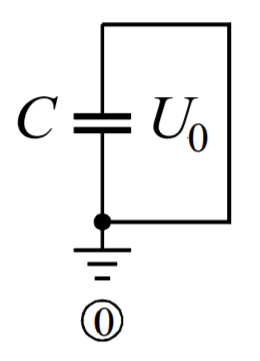
\includegraphics[scale = 0.4]{Figure20.PNG}\\
    Figure 20: Capacitor with initial state - closed circuit.
    \end{center}

    \textbf{Step 16.2.1.} Repeat necessary steps 1.2-1.7.

    \begin{tcolorbox}[breakable, size=fbox, boxrule=1pt, pad at break*=1mm,colback=cellbackground, colframe=cellborder]
\prompt{In}{incolor}{125}{\boxspacing}
\begin{Verbatim}[commandchars=\\\{\}]
\PY{k+kn}{from} \PY{n+nn}{symPyCAP} \PY{k+kn}{import} \PY{n}{Circuit}
\end{Verbatim}
\end{tcolorbox}

    \begin{tcolorbox}[breakable, size=fbox, boxrule=1pt, pad at break*=1mm,colback=cellbackground, colframe=cellborder]
\prompt{In}{incolor}{126}{\boxspacing}
\begin{Verbatim}[commandchars=\\\{\}]
\PY{n}{Capacitor\PYZus{}closed\PYZus{}schematic} \PY{o}{=} \PY{p}{[}
    \PY{p}{[}\PY{l+s+s2}{\PYZdq{}}\PY{l+s+s2}{C}\PY{l+s+s2}{\PYZdq{}}\PY{p}{,} \PY{l+s+s2}{\PYZdq{}}\PY{l+s+s2}{C1}\PY{l+s+s2}{\PYZdq{}}\PY{p}{,} \PY{l+m+mi}{0}\PY{p}{,} \PY{l+m+mi}{0}\PY{p}{,} \PY{l+s+s2}{\PYZdq{}}\PY{l+s+s2}{U0}\PY{l+s+s2}{\PYZdq{}}\PY{p}{]}
\PY{p}{]}
\end{Verbatim}
\end{tcolorbox}

    \begin{tcolorbox}[breakable, size=fbox, boxrule=1pt, pad at break*=1mm,colback=cellbackground, colframe=cellborder]
\prompt{In}{incolor}{127}{\boxspacing}
\begin{Verbatim}[commandchars=\\\{\}]
\PY{n}{Capacitor\PYZus{}closed\PYZus{}circuit} \PY{o}{=} \PY{n}{Circuit}\PY{p}{(}\PY{n}{Capacitor\PYZus{}closed\PYZus{}schematic}\PY{p}{)}
\end{Verbatim}
\end{tcolorbox}

    \begin{tcolorbox}[breakable, size=fbox, boxrule=1pt, pad at break*=1mm,colback=cellbackground, colframe=cellborder]
\prompt{In}{incolor}{128}{\boxspacing}
\begin{Verbatim}[commandchars=\\\{\}]
\PY{n}{Capacitor\PYZus{}closed\PYZus{}circuit}\PY{o}{.}\PY{n}{symPyCAP}\PY{p}{(}\PY{p}{)}
\end{Verbatim}
\end{tcolorbox}

    \begin{tcolorbox}[breakable, size=fbox, boxrule=1pt, pad at break*=1mm,colback=cellbackground, colframe=cellborder]
\prompt{In}{incolor}{129}{\boxspacing}
\begin{Verbatim}[commandchars=\\\{\}]
\PY{n}{Capacitor\PYZus{}closed\PYZus{}circuit}\PY{o}{.}\PY{n}{print\PYZus{}solutions}\PY{p}{(}\PY{p}{)}
\end{Verbatim}
\end{tcolorbox}

    \begin{Verbatim}[commandchars=\\\{\}]
Solution does not exist!
    \end{Verbatim}

    \begin{center}\rule{0.5\linewidth}{0.5pt}\end{center}

    \hypertarget{example-17.1-inductor-with-initial-state---open-circuit}{%
\subsection*{\texorpdfstring{Example 17.1: Inductor with initial state -
open circuit
}{Example 17.1: Inductor with initial state - open circuit }}\label{example171}}

    \begin{center}
    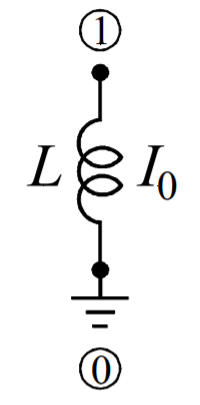
\includegraphics[scale = 0.4]{Figure21.PNG}\\
    Figure 21: Inductor with initial state - open circuit.
    \end{center}

    \textbf{Step 17.1.1.} Repeat necessary steps 1.2-1.7.

    \begin{tcolorbox}[breakable, size=fbox, boxrule=1pt, pad at break*=1mm,colback=cellbackground, colframe=cellborder]
\prompt{In}{incolor}{130}{\boxspacing}
\begin{Verbatim}[commandchars=\\\{\}]
\PY{k+kn}{from} \PY{n+nn}{symPyCAP} \PY{k+kn}{import} \PY{n}{Circuit}
\end{Verbatim}
\end{tcolorbox}

    \begin{tcolorbox}[breakable, size=fbox, boxrule=1pt, pad at break*=1mm,colback=cellbackground, colframe=cellborder]
\prompt{In}{incolor}{131}{\boxspacing}
\begin{Verbatim}[commandchars=\\\{\}]
\PY{n}{Inductor\PYZus{}open\PYZus{}schematic} \PY{o}{=} \PY{p}{[}
    \PY{p}{[}\PY{l+s+s2}{\PYZdq{}}\PY{l+s+s2}{L}\PY{l+s+s2}{\PYZdq{}}\PY{p}{,} \PY{l+s+s2}{\PYZdq{}}\PY{l+s+s2}{L1}\PY{l+s+s2}{\PYZdq{}}\PY{p}{,} \PY{l+m+mi}{1}\PY{p}{,} \PY{l+m+mi}{0}\PY{p}{,} \PY{l+s+s2}{\PYZdq{}}\PY{l+s+s2}{I0}\PY{l+s+s2}{\PYZdq{}}\PY{p}{]}
\PY{p}{]}
\end{Verbatim}
\end{tcolorbox}

    \begin{tcolorbox}[breakable, size=fbox, boxrule=1pt, pad at break*=1mm,colback=cellbackground, colframe=cellborder]
\prompt{In}{incolor}{132}{\boxspacing}
\begin{Verbatim}[commandchars=\\\{\}]
\PY{n}{Inductor\PYZus{}open\PYZus{}circuit} \PY{o}{=} \PY{n}{Circuit}\PY{p}{(}\PY{n}{Inductor\PYZus{}open\PYZus{}schematic}\PY{p}{)}
\end{Verbatim}
\end{tcolorbox}

    \begin{tcolorbox}[breakable, size=fbox, boxrule=1pt, pad at break*=1mm,colback=cellbackground, colframe=cellborder]
\prompt{In}{incolor}{133}{\boxspacing}
\begin{Verbatim}[commandchars=\\\{\}]
\PY{n}{Inductor\PYZus{}open\PYZus{}circuit}\PY{o}{.}\PY{n}{symPyCAP}\PY{p}{(}\PY{p}{)}
\end{Verbatim}
\end{tcolorbox}

    \begin{tcolorbox}[breakable, size=fbox, boxrule=1pt, pad at break*=1mm,colback=cellbackground, colframe=cellborder]
\prompt{In}{incolor}{134}{\boxspacing}
\begin{Verbatim}[commandchars=\\\{\}]
\PY{n}{Inductor\PYZus{}open\PYZus{}circuit}\PY{o}{.}\PY{n}{print\PYZus{}solutions}\PY{p}{(}\PY{p}{)}
\end{Verbatim}
\end{tcolorbox}

    \begin{Verbatim}[commandchars=\\\{\}]
V1 : -I0*L1

    \end{Verbatim}

    \hypertarget{example-17.2-inductor-with-initial-state---closed-circuit}{%
\subsection*{\texorpdfstring{Example 17.2: Inductor with initial state -
closed circuit
}{Example 17.2: Inductor with initial state - closed circuit }}\label{example172}}

    \begin{center}
    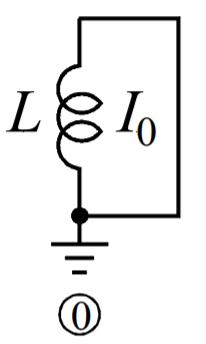
\includegraphics[scale = 0.4]{Figure22.PNG}\\
    Figure 22: Inductor with inital state - closed circuit.
    \end{center}

    \textbf{Step 17.2.1.} Repeat necessary steps 1.2-1.7.

    \begin{tcolorbox}[breakable, size=fbox, boxrule=1pt, pad at break*=1mm,colback=cellbackground, colframe=cellborder]
\prompt{In}{incolor}{135}{\boxspacing}
\begin{Verbatim}[commandchars=\\\{\}]
\PY{k+kn}{from} \PY{n+nn}{symPyCAP} \PY{k+kn}{import} \PY{n}{Circuit}
\end{Verbatim}
\end{tcolorbox}

    \begin{tcolorbox}[breakable, size=fbox, boxrule=1pt, pad at break*=1mm,colback=cellbackground, colframe=cellborder]
\prompt{In}{incolor}{136}{\boxspacing}
\begin{Verbatim}[commandchars=\\\{\}]
\PY{n}{Inductor\PYZus{}closed\PYZus{}schematic} \PY{o}{=} \PY{p}{[}
    \PY{p}{[}\PY{l+s+s2}{\PYZdq{}}\PY{l+s+s2}{L}\PY{l+s+s2}{\PYZdq{}}\PY{p}{,} \PY{l+s+s2}{\PYZdq{}}\PY{l+s+s2}{L1}\PY{l+s+s2}{\PYZdq{}}\PY{p}{,} \PY{l+m+mi}{0}\PY{p}{,} \PY{l+m+mi}{0}\PY{p}{,} \PY{l+s+s2}{\PYZdq{}}\PY{l+s+s2}{I0}\PY{l+s+s2}{\PYZdq{}}\PY{p}{]}
\PY{p}{]}
\end{Verbatim}
\end{tcolorbox}

    \begin{tcolorbox}[breakable, size=fbox, boxrule=1pt, pad at break*=1mm,colback=cellbackground, colframe=cellborder]
\prompt{In}{incolor}{137}{\boxspacing}
\begin{Verbatim}[commandchars=\\\{\}]
\PY{n}{Inductor\PYZus{}closed\PYZus{}circuit} \PY{o}{=} \PY{n}{Circuit}\PY{p}{(}\PY{n}{Inductor\PYZus{}closed\PYZus{}schematic}\PY{p}{)}
\end{Verbatim}
\end{tcolorbox}

    \begin{tcolorbox}[breakable, size=fbox, boxrule=1pt, pad at break*=1mm,colback=cellbackground, colframe=cellborder]
\prompt{In}{incolor}{138}{\boxspacing}
\begin{Verbatim}[commandchars=\\\{\}]
\PY{n}{Inductor\PYZus{}closed\PYZus{}circuit}\PY{o}{.}\PY{n}{symPyCAP}\PY{p}{(}\PY{p}{)}
\end{Verbatim}
\end{tcolorbox}

    \begin{tcolorbox}[breakable, size=fbox, boxrule=1pt, pad at break*=1mm,colback=cellbackground, colframe=cellborder]
\prompt{In}{incolor}{139}{\boxspacing}
\begin{Verbatim}[commandchars=\\\{\}]
\PY{n}{Inductor\PYZus{}closed\PYZus{}circuit}\PY{o}{.}\PY{n}{print\PYZus{}solutions}\PY{p}{(}\PY{p}{)}
\end{Verbatim}
\end{tcolorbox}

    \begin{Verbatim}[commandchars=\\\{\}]
Solution does not exist!
    \end{Verbatim}


    % Add a bibliography block to the postdoc
    
    
    
\end{document}
